% Author: Daniel Celis Garza <daniel.celisgarza@materials.ox.ac.uk>

% Preamble with all the basic packages a thesis would need. Modify as needed.

\documentclass[twoside,htwologo,twosup,12pt]{genthesis}
% By changing the document class this preamble can be used for other document types.
% genthesis.cls contains the definition of the document class.
% Geometry
\usepackage[top=1in, bottom=1in,
	outer=1in, inner=1.5in] % inner = 1.5 for binding
{geometry}

%----------------------- Fonts, symbols and colours ------------------------%
% If using pdfLaTeX comment fontspec and uncomment fontenc and inputenc. If using the superior XeLaTeX/XeTeX or LuaTeX do the opposite.
\usepackage{fontspec}					% XeLaTeX & LuaTeX fonts.
%\usepackage[T1]{fontenc}				% Font encoding for pdfLaTeX
%\usepackage[latin1]{inputenc}			% Input encoding (easy accents) for pdfLaTeX
\usepackage{amssymb, amsmath,
	bm	   , isomath,
	mathtools, esint}					% Maths fonts and symbols.
\usepackage{exscale}					% Removes the need to use {\displaystyle }.
%\newfontfamily\ubuntumono{Ubuntu Mono} % Ubuntu font for fancy shell commands (font needs to be installed).
\usepackage{xcolor}
\usepackage[normalem]{ulem}
%\definecolor{oxfordblue}{cmyk}{79,56,0,72}
\definecolor{oxfordblue}{RGB}{15,31,71}
\usepackage{lmodern}

%------------------------ Hyperlinks and references ------------------------%
\usepackage[colorlinks     = true, % Hyperlinks.
	pdfstartview   = FitV,
	linkcolor      = oxfordblue,
	citecolor      = oxfordblue,
	urlcolor       = oxfordblue,
	hyperfootnotes = true,
	hypertexnames  = true,
	plainpages     = false % Correctly links index entries whenever \thispagestyle{empty} is used.
]{hyperref}
\usepackage[comma  , square,       % Citing style.
	numbers, sort&compress
]{natbib}
\usepackage{cleveref} 			   % Automatic referencing better than \autoref{}.

%----------------------------- Macro utility -------------------------------%
\usepackage{xparse}	 % Expanded macro capability.

%--------------------------- Index and glossary ----------------------------%
\usepackage{makeidx} % Index.
\makeindex			 % Creates index.
\usepackage[toc, acronyms
]{glossaries} % Glossary.
\setglossarystyle{altlisthypergroup} % Sets a list of letters with hyperlinks before the glossaries and acronyms.
% Dual glossary entry.
% Define dual entry for glossary + acronym.
% https://en.wikibooks.org/wiki/LaTeX/Glossary#Dual_entries_with_reference_to_a_glossary_entry_from_an_acronym
\DeclareDocumentCommand{\newdualentry}{ O{} O{} m m m m } {
	\newglossaryentry{gls-#3}{name={#5},text={#5\glsadd{#3}},
	description={#6},#1
}
\makeglossaries
\newacronym[see={[Glossary:]{gls-#3}},#2]{#3}{#4}{#5\glsadd{gls-#3}}
}

%--------------------------------- Utility ---------------------------------%
\usepackage{setspace} % Text spacing commands.
\usepackage{paralist} % In-paragraph lists.
%\usepackage{pdfpages} % Include pdf pages.
%\usepackage{lscape}   % Use landscape pages.
%\allowdisplaybreaks   % Math environments continue onto the next page if they overflow.
\usepackage{siunitx}  % International units.
\usepackage{hologo}   % XeLaTeX and BibTex logos.
\usepackage{ragged2e} % Ragged text.
\usepackage{epigraph}

%--------------------------------- Floats ----------------------------------%
%\usepackage{float} 			% Extra options for floats.
%\usepackage[section]{placeins} % Force floats to stay in the sections they're called in.
\usepackage{booktabs} 			% Nicer tables.
%\usepackage{multirow} 			% Multirow and multicolumn tables. Avoid when possible.
\usepackage{subcaption} 		% Subfigures.
%\usepackage{epstopdf} 			% pdfLaTeX does not support eps images so they need to be converted to pdf.

%---------------------------- Scripts and code -----------------------------%
% If you only need basic script support use verbatim. If you want more features use listings. If you can install pygments use minted.
%\usepackage{verbatim} % Type commands without the hassle of the other two.
%\usepackage{listings} % Spartan display of code and pseudo code.
\usepackage{minted}    % Elegantly display code. Requires a Python 2.7 or higher installation of pygments to be installed. Requires "-shell-escape" flag to the LaTeX compilation command.
\usepackage[chapter]{algorithm}
\usepackage{algpseudocode} % Package for algorithm typesetting (pseudo-code).

%---------------------------- Image file paths -----------------------------%
\graphicspath{{../images/}}

%------------------------------- Input files -------------------------------%
\renewcommand{\vec}{\vectorsym}
\newcommand{\tns}{\tensorsym}
\newcommand{\mtx}{\mathbf}
\newcommand{\mtb}{\textsc{Matlab}}
% Host, device, thread, roman variables.
\newcommand{\hvar}[1]{\ensuremath{^{\textrm{h}}#1}}
\newcommand{\dvar}[1]{\ensuremath{^{\textrm{d}}#1}}
\newcommand{\tvar}[1]{\ensuremath{^{\textrm{t}}#1}}
\newcommand{\rvar}[1]{\ensuremath{\textrm{#1}}}
% \newcommand{\kwdmc}[2]{\gls{#1}\index{\ensuremath{#2}}} % Keyword math command.
% \newcommand{\kwdm}[1]{\gls{#1}\index{\ensuremath{#1}}}  % Keyword math.
% \newcommand{\kwd}[1]{\gls{#1}\index{\gls{#1}}}			% Keyword.
% \newcommand{\kwdp}[1]{\glspl{#1}\index{\gls{#1}}}		% Keyword plural.
% \newcommand{\Kwd}[1]{\Gls{#1}\index{\gls{#1}}}			% Keyword upper case.
% \newcommand{\Kwdp}[1]{\Glspl{#1}\index{\gls{#1}}}		% Keyword plural upper case.
% \newcommand{\kwds}[1]{\glssymbol{#1}\index{\gls{#1}}}	% Keyword symbol.
\newcommand{\nn}{\nonumber\\}							% No number skip line.
\newcommand{\datasepmap}[5]{%
	The data for different #1s of corresponding #2 is separated by \ensuremath{#3} entries. Every time we change #1 we have to skip blocks of size \ensuremath{#4} from \ensuremath{#5}.
}
% \algblockdefx[<block>]{<start>}{<end>}[<startparamcount>][<default value>]{<start text>}[<endparamcount>][<default value>]{<end text>}
\algblockdefx[gpufunction]{GPUFunction}{EndGPUFunction}%
[2][]{\textbf{GPU function} \textsc{#1}(#2)}%
{\textbf{end GPU function}}
% Saves arabic numbering before using the romanpages environment. 
% Add at the end of included chapter so the correct page is recorded.
\newcommand{\savearabiccounter}{
	\setcounter{arabiccounter}{\value{page}}
	%
	\if@twocolumn
		\addtocounter{arabiccounter}{1}
	\else
		\if@openright
			\addtocounter{arabiccounter}{2}
		\else
			\addtocounter{arabiccounter}{1}
		\fi
	\fi
}

\definecolor{matlabOrange}{RGB}{217, 83, 25}
\definecolor{matlabBlue}{RGB}{0, 114, 189}

\DeclareCaptionFormat{algor}{%
	\hrulefill\par\offinterlineskip\vskip1pt%
	\textbf{#1#2}#3\offinterlineskip\hrulefill}
\DeclareCaptionStyle{algori}{singlelinecheck=off,format=algor,labelsep=space}
\captionsetup[algorithm]{style=algori}	 % Macros.
% % Entries without acronyms
\newglossaryentry{bv}
{
	name={Burgers vector},
	description={Denoted as $\vec{b}$, it represents the lattice distortion caused by a dislocation in a crystal lattice. In \emph{edge} dislocations, the Burgers vector is perpendicular to the line direction ($ \vec{b} \perp t $); in \emph{screw} dislocations it is parallel to the line direction ($ \vec{b} \parallel t $); in \emph{mixed} dislocations, Burgers vector and line direction are neither perpendicular nor parallel to each other},
	symbol = {\ensuremath{\vec{b}}}
}

\newglossaryentry{dl}
{
	name={dislocation},
	description={Crystallographic defect which strongly influences many of a material's properties. It can consist of additional or missing partial crystallographic planes, and may come in three varieties: edge, screw and mixed. Mathematically it is a type of topological defect/soliton because it is a distinct, out of equillibrium---but stable---solution of the partial differential equation which in the trivial case yields the crystallographic structure of a material. Like any other soliton, it will not spontaneously decay to the ``trivial'' solution, which in this case would be a perfect crystal. Thus a dislocation preserves its identity by preserving its Burgers vector. Like other solitons, it can annihilate with another of opposite phase, which in this case would be an opposite Burgers vector}
}

\newglossaryentry{devmem}
{
	name = {device memory},
	description = {Graphics card memory visible only within GPU functions}
}

\newglossaryentry{atop}
{
	name = {atomic operation},
	description = {An operation on shared or global device memory which is guaranteed to be performed without interference from other threads. However, atomic operations don't act as memory fences and do not imply thread syncronisation \cite{nvidia_atomics}}
}

\newglossaryentry{thrsync}
{
	name = {thread syncronisation},
	description = {Ensures all threads catch up to each other in some way or another. The function \mintinline{c}{__syncthreads()} ensures all threads in a warp reach the same point. The function \mintinline{c}{__threadfence()} flushes all global memory and shared memory writes by a thread so the updated values are visible to other threads before continuing}
}

\newglossaryentry{cma}
{
	name = {coalesced memory access},
	description = {When all active threads in a warp access contiguous global memory. Therefore cache lines can be very efficiently utilised}
}

\newglossaryentry{wrp}
{
	name = {warp},
	description = {Collection of threads with a maximum of 32 which execute concurrently on the same streaming multiprocessor resources}
}

\newglossaryentry{wrpd}
{
	name = {warp divergence},
	description = {Due to the fact that all threads in a warp must execute the same instruction concurrently, all program branches are executed regardless of branching condition. However, only those instructions for which a branching condition is met have an effect on the state of the thread's program. As a consequence, different threads in a warp may meet different branching conditions, wasting all other branched instructions}
}

\newglossaryentry{tensor}
{
	name = {tensor},
	description = {Geometric object that represents linear relations between matrices, vectors, scalars and other tensors}
}

\newglossaryentry{dls}
{
	name = {dislocation line segment},
	description = {Discretisation of dislocations as straight line segments between two tracked nodes},
	plural={dislocation line segments}
}

% Entries with acronyms
% Syntax: \newdualentry[glossary options][acronym options]{label}{abbrv}{long}{description}
\newdualentry
{sm}
{SM}
{Streaming Multiprocessor}
{A differential equation which contains unkown multivariate functions and their partial derivatives. Solutions require knowledge of the boundary conditions the unkown functions are subject to. The types of PDEs and their boundary conditions can make it difficult or impossible to find well-behaved, analytical solutions. As a result, numerical methods such as finite element method are often used to solve them}

\newdualentry
{pde}
{PDE}
{Partial Differential Equation}
{A differential equation which contains unkown multivariate functions and their partial derivatives. Solutions require knowledge of the boundary conditions the unkown functions are subject to. The types of PDEs and their boundary conditions can make it difficult or impossible to find well-behaved, analytical solutions. As a result, numerical methods such as finite element method are often used to solve them}

\newdualentry
{fem}
{FEM}
{Finite Element Method}
{Also known as finite element analysis (FEA), they are a class of numerical methods for solving boundary value problems for partial differential equation whose analytical solution might not meet the necessary uniqueness and existence requirements of a physical problem. These methods divide the domain of interest into smaller, simpler subdomains that can be described by a system of algebraic equations. These are then assembled into a larger system of coupled algebraic equations that approximately model the whole domain. Variational methods are then used to find an approximate solution by minimising an associated error function}

\newdualentry
{bem}
{BEM}
{Boundary Element Method}
{The 2D analogue of an finite element method, where only the domain boundaries are of interest}

\newdualentry
{fe}
{FE}
{Finite Element}
{One of the subdomains of a problem solved via finite element method}

\newdualentry
{be}
{BE}
{Boundary Element}
{One of the subdomains of a problem solved via boundary element method}

\newdualentry
{se}
{SE}
{Surface Element}
{Special case of a boundary element, where the boundary is a surface}

\newdualentry
{ddd}
{DDD}
{Discrete Dislocation Dynamics}
{The study of the dynamics of dislocations as discrete entities made up of discrete nodes connected by line segments. They assume an infinite medium in which dislocations exist, evolve and interact. Due to their intermediate nature between atomistic and continuum models, they can explore time and length scales which are either too big for more fundamental approaches, and too small for finite element method} % Glossaries.

%----------------------------- Special options -----------------------------%
%\counterwithout{figure}{chapter} % Uncomment to remove chapter number from figures.
%\counterwithout{table}{chapter}  % Uncomment to remove chapter number from tables.
%\setlength{\topskip}{0in}        % Top paragraph spacing.
%\setlength{\parskip}{2ex}        % Bottom paragraph spacing.
%\linespread{1.5} 				  % Inter-line spacing (1 = single space, 1.5 = double space).
%\renewcommand{\footnoterule}{% Footnote fule that spans the whole textwidth.
%	\kern -5.4pt
%	\hrule width \textwidth height 0.4pt
%	\kern 5pt
%}
%\makeatletter \newcommand*{\codefont}{% \codefont provides font size for code (for use in listings and minted).
%	\@setfontsize
%	\codefont{10pt}{11pt}
%}\makeatother
\title{Dislocation Based Modelling of Fusion Relevant Materials.}
\logo{2.5in}{./images/ox_brand_cmyk_pos.eps}{2.5in}{./images/hmc.eps}
\author{Daniel Celis Garza}
\university{University of Oxford}
\college{Harris-Manchester}
\department{Materials}
\supervisor{Edmund Tarleton}{Angus Wilkinson}
\degree{Doctor in Philosophy}
\degreedate{Trinity Term 2020}
\begin{document}
\maketitle
\onehalfspacing
% Front matter.
\begin{frontmatter}[Dedication]

    \centering
    ``Ohana significa familia, y tu familia nunca te abandona, ni te olvida.''\\
    ``Ohana means family, family means nobody gets left behind, or forgotten.''\\
    -- Stitch, Lilo \& Stitch

    \justify
    Malle santa, cuando te hablé desde el trabajo para darte la noticia me dijiste que siempre lo supiste. Recuerdo que lloraste en el teléfono, se te cerró la garganta y a mí también. A diferencia de otras veces, no pudimos platicar mucho porque nos quedamos sin aliento. Así que le hablaste a abuelita Raquel mientras le hablé a papá. Madre, David y yo te debemos tanto que no podemos repagar en mil vidas, pero ten por seguro que eres nuestro ejemplo a seguir. Nuestra madre chingona y chambeadora, solo hay una y como ella no hay ninguna. Sin tí el mundo sería un lugar más cruel y pobre, no merece un ángel tan grande y puro como tú.

    Dad, ``Igualito que tu jefe, wey.'' con tu risa característica fue lo primero que dijiste cuando te avisé ``Sí dad, igualito que mi jefe.'' entre risas respondí. Como siempre, no platicamos mucho pero esta vez porque le querías avisar a abuelita Teté y a mis tíos, y yo le quería avisar a David. Pensé que seguirías aquí para carcajearte al verme en la túnica ridícula, así como lo hicimos nosotros cuando te vimos a tí en la tuya. Escribo esta dedicatoria antes de acabar porque una promesa es una promesa y esta madre la voy a acabar. No te tendré para pedirte consejos y contarte mis avances y tropiezos. Pero a veces pretendo que me escuchas mientras intento comprender o arreglar algo. Te queremos y te extrañamos muchísimo. Buenas noches, dad.

    David, ``Te mamaste we.'' me dijiste cuando me abrazaste al llegar a casa después del trabajo el día que me aceptaron. Me has hecho un chingo de falta ojete, te extraño mucho we. Perdón por no hablar tan seguido, pero me duele colgar we. No estoy tan chisqueado como mamá pero siento feo cuando terminamos de platicar. Me gusta mucho ver tus streams porque me recuerda un poco a sentarme a tu lado a verte jugar\ldots{} o a cuando veíamos Twitch juntos y veíamos a TB missing legal.

    Esto es para mi Ohana por sangre y por elección. Ustedes creyeron en mí cuando yo no lo hacía. Me empujaron a ser mejor. Me extendieron la mano cuando nadie más lo hizo. Me hicieron reir cuando solo sabía llorar. Gracias por hacerme quien soy.

    This is for my Ohana by blood and by choice. You believed in me when I did not. You pushed me to be better. Offered me a helping hand when nobody would. Made me laugh when all I knew was sorrow. Thank you for making me who I am.
\end{frontmatter}

\begin{frontmatter}[Acknowledgements]
    \centering
    ``You can always judge a man by the quality of his enemies.''\\
    -- Oscar Wilde

    \justify
    I did not get here alone. Truly I don't have much idea what I did to deserve the help and encouragement of such an eclectic mix of awesome people. The list is long, but like the proverbial beating of a butterfly's wings, there is no telling where I'd be without the aid and support of these people.
    \begin{itemize}
        \item Ed and Angus
        \item Fusion CDT
        \item Harris-Manchester
        \item CONACYT
        \item Anatoly Kolomeisky, John F. Stanton
        \item Isla
        \item Clan del Rano Sentado
        \item Goosehood
        \item Kopse Lane Krump v1.0 v2.0
        \item Kristmas Karnage: n
        \item OUPLC: Perhaps the heaviest things that we lift are not our weights, but our feels.
        \item Damian Rouson
        \item Bruce Bromage, Haiyang Yu, Fenxian Liu, Daniel Hortelano-Roig, Junnan Jiang
    \end{itemize}

    I guess I'll content myself with being judged unfavourably by the world.
\end{frontmatter}
% Table of contents.
\setcounter{secnumdepth}{3}
\setcounter{tocdepth}{3}
\begin{romanpages}
	\tableofcontents
	%
%	\ifnum\value{figure}>0
	\phantomsection
	\addcontentsline{toc}{chapter}{List of Figures} % Add table index to the table of contents (toc).
	\listoffigures
%	\fi
	%
%	\ifnum\value{table}>0
	\phantomsection
	\addcontentsline{toc}{chapter}{List of Tables} % Add table index to the table of contents (toc).
	\listoftables
%	\fi
	%
%	\ifnum\value{algorithm}>0
	\phantomsection
	\addcontentsline{toc}{chapter}{List of Algorithms} % Add table index to the table of contents (toc).
	\listofalgorithms
%	\fi
	%
	\printglossary[type=\acronymtype,title={Abbreviations}]
\end{romanpages}
% Middle matter.
% TODO #8
\chapter*{Outline}
\begin{enumerate}
    \item Lit review
    \item DDD-FEM
    \item Analytic tractions
          \begin{enumerate}
              \item Traction errors
              \item Reaction force errors
              \item Simulations
              \item Recommendations and Conclusions
          \end{enumerate}
    \item Parallelising tractions
          \begin{enumerate}
              \item Algorithms
              \item Performance
              \item Simulations
              \item Recommendations and Conclusions
          \end{enumerate}
    \item EasyDD v2.0
          \begin{enumerate}
              \item Adaptive integration
              \item New mobility law
              \item Surface velocities
              \item Collisions
              \item Code redesign
          \end{enumerate}
    \item Future work
          \begin{enumerate}
              \item Julia redesign
              \item Preliminary comparisons
          \end{enumerate}
    \item Conclusions
\end{enumerate}
\addtocounter{chapter}{-1}
\chapter{Preface}
\label{c:pre}

\section{Notation and abbreviation}
\label{s:nota}

For the sake of clarity the following notation and abbreviation conventions have been used:
\begin{itemize}
	\item GPU: Graphics Processing Unit.
	\item CPU: Central Processing Unit.
	\item Tensors are denoted by sans serif bold italics, $ \tns{T} $.
	\item Matrices are denoted by serif bold roman, $ \mtx{M} $.
	\item Vectors are denoted by serif bold italics, $ \vec{V} $.
	\item Scalars are denoted by serif italics, $ S $.
	\item Operators and special functions are roman, $\exp(x)$, $\det{\mtx{J}}$.
	\item Angles are in radians unless otherwise stated.
	\item Einstein notation for tensor components is used unless otherwise stated.
	\item Individual items, be they nodes, surface elements, dislocation segments or indices are denoted by a lower-case subscript to the right, $a_n$.
	\item Ensembles are denoted by an upper-case subscript to the right, $a_N \coloneqq \sum a_n$.
	\item Host variables (CPU variables in parallelisation) are denoted by a roman h-superscript on the left, $\hvar{a}$.
	\item Global device variables (global variables visible only to the GPU) are denoted by a roman d-superscript on the left, $\dvar{a}$.
	\item Thread variables (variables visible only to a GPU thread) are denoted by a roman t-superscript on the left, $\tvar{a}$.
	\item Serial indices/counters are the traditional $i$, $j$, $k$\ldots{}.
	\item Parallel indices are denoted as roman variables, $\rvar{a}$.
	\item Pseudo-code is C-style---row-major order, 0-based indexing---because it provides a more direct translation of the C-code.
\end{itemize}

\section{Typesetting}
\label{s:typeset}

The repository \href{https://github.com/dcelisgarza/latex_templates}{https://github.com/dcelisgarza/latex\_templates} contains the custom document class used to typeset this document. It was compiled with \hologo{XeLaTeX} and \hologo{BibTeX}. We recommend compiling the source with \hologo{XeLaTeX} or \hologo{LuaLaTeX}. Compilation requires \texttt{minted}, \href{https://ctan.org/pkg/minted?lang=en}{https://ctan.org/pkg/minted?lang=en}, and its dependencies.
\section{Diagrams}
\label{s:diag}

All diagrams were drawn with Inkscape: Open Source Scalable Vector Graphics Editor, \href{https://inkscape.org/}{https://inkscape.org/}, ``Draw Freely.''
\savearabiccounter
% 259 words
% TODO #7
\chapter{Introduction}
\label{c:intro}
\section{Materials Science and History}
\label{s:matsci_history}
Metals and alloys are of such importance to humankind that entire eras of our history have been defined by and named after discoveries and advances in metallurgy \cite{metals_prehistory1, metals_prehistory2}. A civilisation's ability to gain mastery of the properties and usage of materials is often strongly correlated with its success in history \cite{metals_success1}. The historical influence of metals and alloys has touched all areas of human existence, from fashion to warfare \cite{metals_social}.

It should come as no surprise that a material's use is often linked to its properties. When a civilisation learned to harness the properties of a novel material, its influence often grew as a result \cite{guns_germs_steel, metals_success2}. Whether building a woodcutter's axe or a fusion reactor, the mechanical behaviour and deformation of materials---metals and alloys in particular---are still among their most important properties for engineering applications.

Traditionally such properties have been largely studied via empirical methods such as tensile and compressive tests, beam bending, and indentation \cite{tensile_test_theory, bending_test_theory, indentation_theory}. Such tests have mainly focused on macroscopic scales, thus offering bulk-averaged properties valuable for engineers. Unfortunately such tests only describe observed behaviours without truly elucidating the fundamental mechanisms behind them \cite{micromech_test1}. This has recently started to change with the advent of micro-scale testing, where tests can be performed on single crystals or individual crystal boundaries, and can even probe specific slip systems to see how they behave under various loading scenarios \cite{micromech_test2, micromech_test3}. The increased resolution and more thorough parameter control goes a long way in providing a window through which more fundamental behaviours can be observed and hopefully explained; thus providing a way of deconvoluting macroscopic observations into their constituent phenomena \cite{micro_macro1, micro_macro2}.

However, understanding the underlying mechanisms behind empirical results through experimental means has proven difficult at every scale \cite{multiscale_model_mats1, multiscale_model_mats2}. Fortunately modelling and simulation can be powerful allies in this task. In particular, the study of dislocations is experimentally challenging \cite{dln_exp_obs1, dln_exp_obs2, dln_exp_obs3}. By virtue of being such an important player in the mechanical properties of materials, dislocations demand careful study from both empirical and in-sillico avenues.

The need for a more detailed picture of material properties is especially relevant in highly engineered alloys subjected to extreme conditions, such as those found in fusion reactors. The time-dependent shift in material properties and composition is of the utmost concern such extreme environments; radiation damage, large temperature gradients, gas diffusion and plasma instabilities provide the means for properties to change drastically over a components' lifetime \cite{fusmat1, mats_fusion1, mats_fusion2}. It is therefore imperative that we find ways of predicting and accounting for these changes. This requires a deeper understanding of the process driving the mechanical behaviour. Virtual experiments allow analysis and interpretation of micromechanical tests and can help provide new fundamental insight.

\section{Fusion Energy Production}
\label{s:fusion}
There currently exist two major branches of research for fusion energy production \cite{icfvsmcf}:
\begin{inparaenum}[\itshape1\upshape)]
	\item magnetic confinement fusion (MCF) \cite{mcf} which confines the plasma using magnetic fields and
	\item inertial confinement fusion (ICF) \cite{icf} which uses a frozen fuel pellet which is either directly or indirectly compressed by arrays of powerful lasers.
\end{inparaenum}
The physics and engineering challenges vary greatly between both approaches but the fundamental materials problems remain largely the same, with few a exceptions such as divertors \cite{icf_mcf1, icf_mcf2}.

\subsection{Operating environment}
\label{ss:operating_env}
One constant feature of nuclear energy production is ionising and non-ionising radiation. In the case of fission, this is mostly in the form of low energy neutrons and residual radiation of fission products; fusion on the other hand, deals with the sparsely explored 14 MeV neutron spectrum \cite{mats_fis_fus}. The lack of appropriate sources of suitably energetic neutrons \cite{ifmif} has meant that modelling, and searching for experimental analogues of damage cascades have become a crucial part of materials research \cite{fusmat1s}.

Operating environments change vastly between ICF and MCF as described by \cref{tab:rad} \cite{openv}. The table should be read with a measure of skepticism as the numbers and conditions are approximate because they are not yet fully known, especially for ICF. However it is still, a fairly reasonable first approximation into the materials requirements for both ``mainstream'' types of fusion energy production. That said, the components needed for energy harvesting---a divertor in the case of MCF, and an open problem for ICF---are conspicuous by their absence.

\begin{table}
	\centering
	\resizebox{\textwidth}{!}{
		\begin{tabular}{llrr}
			\toprule
			Location                         & Radiation Type          & MCF (ITER)                   & ICF (LMJ)                                                                               \\
			\midrule
			1\textsuperscript{st} Wall       & Neutron flux            & \SI{3e18}{m^{-2}.s^{-1}}     & \SI{1.5e25}{m^{-2}.s^{-1}}                                                              \\
			                                 & Neutron fluence*        & \SI{3e25}{m^{-2}}            & \SI{3e18}{m^{-2}}                                                                       \\
			                                 & $\gamma$-ray dose rate  & \SI{2e3}{\gray.s^{-1}}       & $\sim$ \SI{1e10}{\gray.s^{-1}}                                                          \\
			                                 & Energetic ion/atom flux & \SI{5e19}{m^{-2}.s^{1}}      & \ldots                                                                                  \\
			\midrule
			1\textsuperscript{st} Diagnostic & Neutron flux            & \SI{1e17}{m^{-2}.s^{-1}}     & \SI{1e26}{m^{-2}.s^{-1}}                                                                \\
			                                 & Neutron damage rate     & \SI{6e-9}{dpa.s^{-1}}        & negligible                                                                              \\
			                                 & Neutron fluence*        & \SI{2e24}{m^{-2}}            & $\sim$\SI{1e19}{m^{-2}}                                                                 \\
			                                 & Neutron damage          & \SI{1e-1}{dpa}               & negligible                                                                              \\
			                                 & $\gamma$-ray dose rate  & $\sim$\SI{1e2}{\gray.s^{-1}} & $\sim$\SI{1e10}{\gray.s^{-1}}                                                           \\
			                                 & Energetic ion/atom flux & $\sim$\SI{1e18}{m^{-2}}      & \ldots                                                                                  \\
			                                 & Nuclear heating         & \SI{1}{\mega\watt.m^{-3}}    & 0                                                                                       \\
			                                 & Operating temperature   & \SI{520}{\kelvin}            & \SI{293}{\kelvin}                                                                       \\
			                                 & Atomosphere             & Vacuum                       & Air                                                                                     \\
			\midrule
			Other                            & EM pulse                & \ldots                       & \SIrange[range-units = single]{10}{500}{\kilo\volt.m^{-1}} @ \SI{1}{\giga\hertz}        \\
			                                 & Shrapnel                & \ldots                       & \SIrange[range-units = single]{1}{10}{\kilo\metre.s^{-1}} @ $\sim$\SI{30}{\micro\metre} \\
			\bottomrule
		\end{tabular}
	}
	\caption[Estimated operating conditions of MCF and ICF fusion reactors.]{Estimated operating environment comparison between MCF (ITER) and ICF (LMJ). Reproduced from \cite{openv}. Note these numbers are unrepresentative of actual fusion power plants as both ITER and the LMJ are experiments---it is likely power plants will require much harsher operating conditions.\\ * End of life.}
	\label{tab:rad}
\end{table}

\Cref{tab:rad} shows that dosages and dosage rates vary wildly between approaches. For the most part, MCF receives higher doses of neutrons and ions in both the first wall and diagnostic equipment. This seems to indicate that the material requirements for MCF are stricter than for ICF. However, shrapnel production is a strong possibility in ICF, especially in indirect drive reactors; where a specially made container called a ``hohlraum'' holds the fuel pellet and is subsequently obliterated when the pellet undergoes fusion (see \cref{fig:hohlraum} \cite{hohlraum}). This is a huge challenge as such high energy shrapnel would be capable of destroying diagnostic equipment and damaging the first wall \cite{icfpwr1,icfpwr2,icfpwr3}.

\begin{figure}[t]
	\centering
	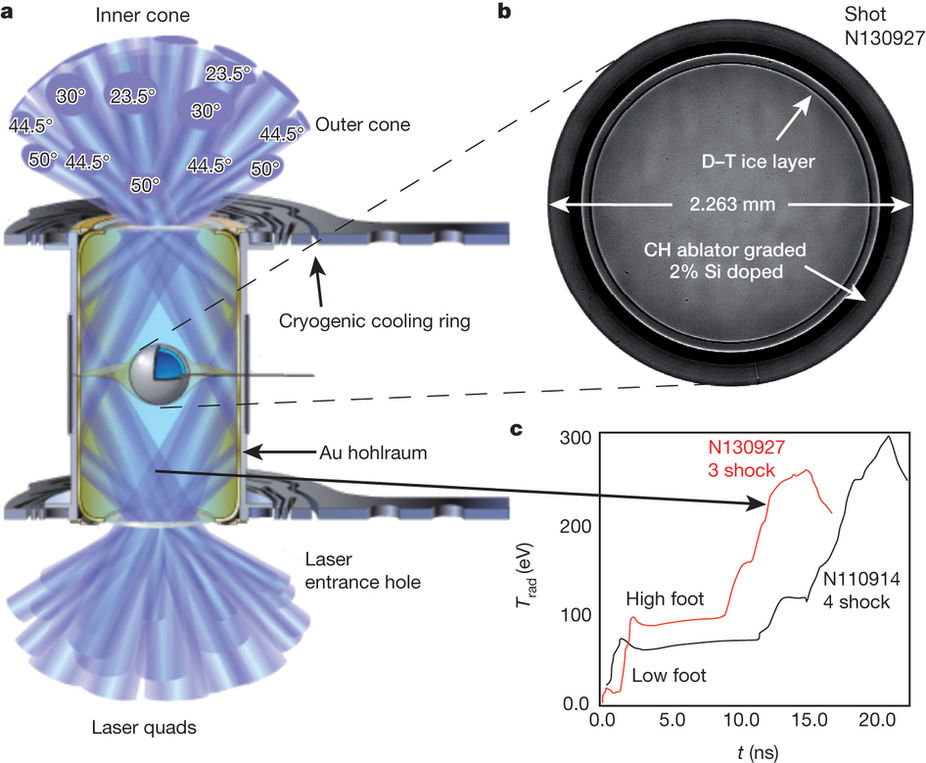
\includegraphics[width=\linewidth]{hohlraum.jpg}
	\caption[Hohlraum design for indirect drive in Inertial Confinement Fusion.]{\textbf{a}, Cross section of the National Ignition Facility's ICF target design showing the gold hohlraum and plastic capsule, fuel pellet, and incident laser bundles. \textbf{b}, X-ray image of the actual capsule for N130927 with DT fuel layer and surrounding CH (carbon–hydrogen) plastic ablator. \textbf{c}, X-ray radiation drive temperature as a function of time for the National Ignition Campaign (NIC) low-foot implosion and the post-NIC high-foot implosion. Image taken from \cite{hohlraum}.}
	\label{fig:hohlraum}
\end{figure}

Overall, the table is unrepresentative of potential operating environments in large-scale power stations, but sets lower limits on the demands of the materials involved in both ``mainstream'' proposals for fusion energy production.

\subsection{Effects of Radiation on Reactor Materials}
\label{ss:rad_effect_mat}
\subsubsection{Radiation Damage}
\label{sss:rad_damage}
One of the bigger problems in radiation damage research is the lack of a truly standardised way of measuring damage on materials \cite{srimisbad}. The most common unit is displacements per atom (dpa) \cite{dpa}. It is defined as the average number of displacements undergone by each atom in a material as a result of being irradiated. The ``fundamental'' unit of measurement for this is the number of displacements per unit volume per unit time, $R$
\begin{align}
	R & = N\int _{E_{\rvar{min}}}^{E_{\rvar{max}}}\int _{T_{\rvar{min}}}^{T_{\rvar{max}}}\phi (E)\,\sigma (E,T)\,\upsilon (T)\;\rvar{d}T\;\rvar{d}E\;,
\end{align}
where $ N $ is the atom number density (no. of atoms per unit volume); $ E $ the incoming particle's energy; $ T $ the energy transferred in a collision of a particle of energy $E$ and a lattice atom; $ \phi(E) $ the energy dependent particle flux; $ \sigma(E,T) $ the cross section for the collision of a particle with energy $ E $ resulting in a transfer of energy $ T $ to the struck atom; and $ \upsilon(T) $ the number of displacements per primary knock on atom as a function of transferred energy $ T $. DPA can be calculated by na\"{i}vely multiplying $ R $ by the sample volume and total exposure time (or we could use fluence rather than flux). This ignores the fact that $\sigma (E,T)$ and $\upsilon (T)$ will be locally perturbed in the neighbourhood of damage cascades, since the bulk volume is much greater than that of the damage cascades', we assume the functions remain globally unchanged.

In principle, this is a rather good measure of damage \cite{dpa}. The catch is that generalised, analytical expressions for $ \sigma(E,T) $ and $ \upsilon(T) $ depend on a slew of parameters and are therefore incredibly hard if not impossible to derive. This does not mean they cannot be discretised and roughly approximated via Monte Carlo (MC) approaches \cite{srim, srimisbad, dpa}. However, damage cascade modelling falls squarely in the realm of pico- to nanosecond timescales and as such only feasable with Molecular Dynamics (MD) and Kinetic Monte Carlo (KMC) \cite{dmg_cascade1, dmg_cascade2} approaches. At the end of such cascades, we are often left with dislocation sources or prismatic dislocation loops \cite{dmg_cascade_dln} which can be used as inputs by a Dislocation Dynamics (DD) simulation to study larger temporal and spatial scales \cite{fusmat1s}.

\subsubsection{Transmutation}
\label{sss:transmutation}
Transmutation products are one of the biggest sources of problems for materials in fusion applications \cite{fusmat1, mats_fusion1}. Not only do they tend to embrittle materials, they often also reduce their thermal conductivity \cite{transmute}. The former presents significant challenges for structural materials \cite{ods_rad_res}; the latter is especially egregious for energy extraction by limiting the divertor's ability to conduct heat thus lowering the reactor's efficiency and causing thermal stresses due to the generation of hot spots that cannot be easily dissipated. As a result, understanding the mechanical and thermal behaviour of transmutation alloys is crucial for moving forward \cite{nirrhard, colcas, hardening} but doing so requires knowledge of the time evolution of a reactor's components. Because the composition changes in a a non-trivial way, so do the mechanical properties. Worse still are the long timescales over which this happens---on the order of years or tens of years \cite{transmute2}. Even if we were able to expermentally irradiate fusion-relevant materials with appropriately energetic neutrons, it would take years before we could characterise their behaviour, and doing so would be problematic due to radioactive decay.

The way we go about addressing the time-dependent compositional change of a material is to model it. Culham Centre for Fusion Energy's (CCFE) FISPACT \cite{fispact} software takes an MC approach at calculating transmutation and decay products of a sample given certain conditions. The code utilises external data provided by the European Activation File which provides cross sections and decay rates for a wide range of isotopes \cite{fispact_library}. Unfortunately there is a lack cross section data for certain neutron energies that contribute in a non-negligible manner to a fusion environment. Interpolating to fill the gaps would not be appropriate as the data is non-smooth and subject to resonance peaks, so the solution is imperfect.

Transmutation products will always be problematic, but they are a fact of working with fusion-relevant materials. Fortunately there are ways in which inclusions may be modelled via DD (\cref{sss:inclusions}). DD may also be used to model dislocation movement and interaction within heterogenous media (\cref{ss:multiphase}) as is the case for oxide-dispersion-strengthened (ODS) steels; and transmutation alloys of Tungsten divertors, where Osmium, Rhenium and Tantalum clusters which prove highly problematic for its temperature conductivity and structural integrity \cite{w_cluster1, nirrprop, nirpropmic, nirrmic, ionirrmic, ionirrprop, ionirrprop2}.

\section{Parallel Computing}
\label{s:parallel_comp}
Processing chips are made up of millions or even billions of transistors acting as switches in logic gates. Each time a logic gate fires, the capacitors inside them charge and discharge at the chip's frequency or clock speed \cite{cpu_trnstor}. Consider the power of any electronic component,
\begin{align}
	P(t) & = I(t) V(t) \label{eq:pow_ec} \,,
\end{align}
where $ I $ is current and $ V $ is voltage both as a function of time. The current, $ I $, of a capacitor and the definition of power, $ P $, as functions of time, $ t $, are given by,
\begin{align}
	I(t) = C \dfrac{\mathrm{d}V(t)}{\rvar{d}t} \label{eq:cap_cur_pow_dt}\,, \qquad
	P(t) = \dfrac{\rvar{d}E(t)}{\rvar{d}t}\,,
\end{align}
where $ C $ is capacitance and $ E $ the energy stored in the capacitor. Substituting \cref{eq:cap_cur_pow_dt} into \cref{eq:pow_ec} and integrating twice, we obtain the expression for the energy stored in a capacitor,
\begin{align}
	%		\int\limits_{0}^{E_{c}}\int\limits_{0}^{\infty} \dfrac{\rvar{d}E(t)}{\rvar{d}t}\; \rvar{d}t &= C \int\limits_{0}^{V_{c}}\int\limits_{0}^{\infty} V(t) \dfrac{\mathrm{d}V(t)}{\rvar{d}t}\; \rvar{d}t\\
	E_{\rvar{c}} & = \dfrac{C V_{\rvar{c}}^{2}}{2} \label{eq:e_cap}\,,
\end{align}
where $ V_{\rvar{c}} $ and $ E_{\rvar{c}} $ are the voltage and energy stored in the capacitor. Recalling that in a processing chip, the capacitors are charged and discharged at the chip's clock speed $ f $, we arrive at the expression for power consumption, $ P_{\rvar{c}} $, of a capacitor charging and discharging at frequency $ f $ \cite{microelec},
\begin{align}
	P_{\rvar{c}} & = E_{\rvar{c}} f \propto C V_{\rvar{c}}^{2} f \label{eq:p_cap}\,.
\end{align}

Computer chips are rather more complicated, but their power consumption (also known as power dissipation) is described by a simple addition of terms \cite{cpu_pow},
\begin{align}
	P = P_{\rvar{dyn}} + P_{\rvar{sc}} + P_{\rvar{leak}}\,,
\end{align}
where $ P_{\rvar{dyn}} $ is the dynamic power dissipation given by \cref{eq:p_cap}. The two other dissipation mechanisms are:
\begin{inparaenum}[\itshape 1\upshape)]
	\item short-circuit, sc, which depends on frequency and occurs when a direct path from transistor to ground is made as a result of multiple transistors conducting simultaneously; and
	\item leakage, leak, which depends on the voltage and is due to micro-currents between doped parts a transistor.
\end{inparaenum}
Furthermore, higher voltages and frequencies result in higher temperatures, which in turn mean decreased transistor performance and increased capacitance. The overall result is an energy expenditure curve similar to \cref{fig:cpu_en_cnvx} \cite{cpu_en_cnvx} for every processor unit.
\begin{figure}[t]
	\centering
	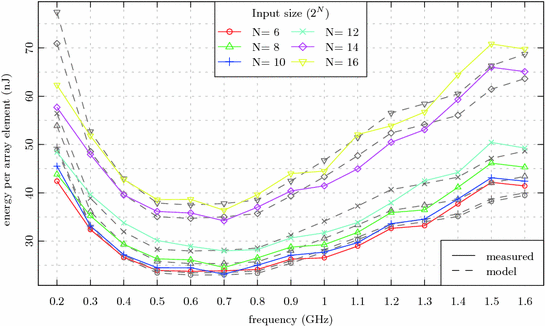
\includegraphics[width=\linewidth]{cpu_en_cnvx.png}
	\caption[Energy expenditure of CPU vs Voltage.]{Energy required by a Samsung Galaxy S2 CPU at \SI{37}{\degreeCelsius} to complete the Gold-Rader implementation of the \emph{bit-reverse} algorithm. The dashed lines denote a theoretical model, image and model found in \cite{cpu_en_cnvx}.}
	\label{fig:cpu_en_cnvx}
\end{figure}

This set of optimum conditions is the reason behind the multicore and multithreaded design of modern Central Processing Units (CPUs) and Graphics Processing Units (GPUs). It is also why in recent years there has been such a massive push for parallelism in all computing markets. It is simply not feasable to continually increase clock speeds and voltages because cooling solutions would struggle to remove heat fast enough, and power consumption would skyrocket.

\section{Computation on Graphics Processing Units}
\begin{figure}[t]
	\centering
	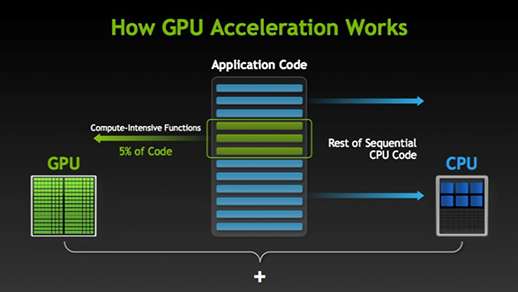
\includegraphics[width=\linewidth]{gpu_parallel.png}
	\caption[CUDA runtime schematic.]{CUDA runtime schematic. Repetitive but computationally intensive tasks can be offloaded to the GPU. Both GPU and CPU are completely independent from each other and can work on different parts of the code at the same time, care must be taken to ensure proper syncronisation. Image taken from \cite{nvidia}.}
	\label{fig:cuda}
\end{figure}

Central Processing Units (CPUs) are designed not only to perform mathematical operations but logical ones that control program flow. They are tailored to perform the wide variety of operations required by an operating system. These include program scheduling (load balancing), instantiation (program loading, unloading, loops, recusion instances) \& branching (if/case statements, go to's), memory operations (fetching, storing, allocation), input/output (IO), and program monitoring (program counters, recursion counters). Modern CPUs have a degree of parallelism that allows them to increase their total throughput while keeping their operation within near optimum conditions as previously mentioned. They are commonly divided into cores and threads, though certain high-end chips have an additional layer named hyperthreading \cite{cpu_arch}.

Given the limited scope of the first computers, the general purpose of CPUs was enough to cover their needs. With the advent of personal computers, the demands on CPUs drastically increased. For industrial users these revolved around data acquisition, filtering and preprocessing \cite{fpga, preproc, filtering}. On the other hand, the domestic market demanded ever increasing levels of abstraction and usability in the form of Graphical User Interfaces (GUIs) such as windows, cursors and their accompanying sound effects. Manufacturers identified this and moved to provide specialised modules that freed CPU resources and improved user experience by accelerating different processes through hardware means \cite{gpu1, gpu2, gpu3, sound}. These modules include Sound Cards (SCs), Field Programmable Gate Arrays (FPGAs), Graphics Processing Units (GPUs), Application Specific Integrated Circuits (ASICs), Cryptographic Accelerators, Regular Rxpression (RegEx) Accelerators, among others. They are collectively dubbed ``hardware accelerators''.

Graphics Processing Units were originally intended to offload the very data-intensive but computationally simple operations needed for 3D gaming and rendering \cite{gpu1, gpu2, gpu3}. Graphics processing was seen as a prime candidate for hardware acceleration because the operations on each pixel are largely the same across the screen. Due to their original purpose as gaming and rendering accelerators, they were never designed to operate on higher than single precision data. In fact, single precision (32-bit precision) is still good enough to encode 32-bit colour depth (8-bit channel per RGB colour + 8-bit alpha channel), which only the most high-end monitors support \cite{monitor}. It is also worth noting that because the same operations apply to different pieces of (mostly) independent data, they can all be performed at the same time, often trivially reducing the order of polynomial complexity algorithms.

As previously mentioned, GPU parallelism frees up enormous amounts of CPU processing power that can be put to good use running other programs or performing complementary serial processes, while the GPU works concurrently on its dataset. Parallelism has been used by the scientific community for years, but the focus has mainly been on CPU parallelism \cite{cpu_par}. Consequently, its scope was lagerly limited to the use of computational clusters. The two main reasons for this were the fact that GPUs lacked support for higher precision arithmetic, and the very limited to non-existent support for scientific computing in languages such as OpenGL \cite{gpu_comp}.

It wasn't until the development of the OpenCL and OpenACC standards that GPUs caught the attanetion of the scientific community as a viable way of exploiting parallelisation without access to a computing cluster.

OpenCL allows one to work with heteragoenous systems and is similar to C in that it's very low level. It works on a wide range of hardware accelerators and is therefore useful for many scientific and engineering applications, but it's also relatively hard to use. One can make use of libraries written in OpenCL to facilitate development, but it is still a fully fledged C-type language \cite{opencl}.

OpenACC is similar to OpenMP in that they both use pragmas\footnote{Pragmas are especially formated comments that specific compilers recognise and turn into special instructions (often for moving memory to the appropriate hardware) at compile time. They are not part of the programming language's official standard, but rather compiler-specific extensions. Pragmas are usually programmed in C or Assembly and must be implemented by the compiler manufacturer. Nothing prevents application developers from writing the would-be pragma's code directly into their application, but this can prove a lengthy and difficult process. The rigid nature of pragmas, and the compiler manufacturer's priorities limit their scope and usability.} and they both work in shared memory environments---same GPU and same CPU respectively. This is no coincidence as OpenACC was designed as an extension of OpenMP for developing parallel applications on hardware accelerators. Unfortunately, being pragma based, the standard requires significant work by compiler manufacturers, so its adoption has therefore been slow \cite{openacc}. Furthermore, despite simplifying development and minimising the barrier to entry, the use of pragmas limits the flexibility and adaptability of the framework compared to OpenCL.

Recently however, a third option has become increasingly viable. NVidia's Computer Unified Device Architecture (CUDA) framework provides the best aspects of both OpenCL and OpenACC. The tradeoff is that it only works on NVidia GPUs and is a closed source product. However, the accessibility and flexibility of CUDA provides anyone familiar with C/C++ the means to develop a GPU application with little issue. NVidia is also strongly backing scientific research by adding double precision support on their GPUs. They have also worked to provide parallel equivalents of well known serial libraries---such as cuBLAS \& cuFFT---for scientific computing. They have additionally developed a wide range of specialist graphics cards tailor-made for scientific purposes. As such, they are the leaders in GPU computing in scientific communities \cite{nvidia}.

\subsection{Hurdles for Parallelisation}
\begin{figure}[t]
	\centering
	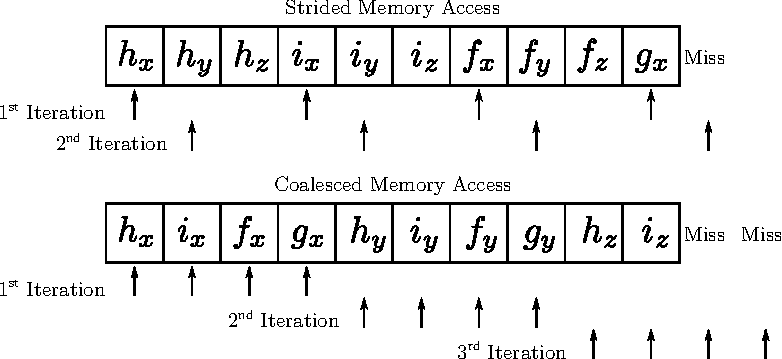
\includegraphics[width=\linewidth]{mem_access.pdf}
	\caption[Memory access pattern example.]{Arrows represent fetch requests by single threads in a GPU. Data should be arranged in such a way that all threads in a warp (collections of 32 threads) access contiguous memory locations to reduce time-consuming memory fetch operations. This is often unintuitive but extremely important, especially on scientific computing cards which are optimised for long computational times and low memory fetch frequency.}
	\label{fig:mem_access}
\end{figure}

The difficulty in parallelisation varies tremendously from problem to problem. Problems where data is uncorrelated and independent---such as sampling well-behaved probability distributions---are almost trivially parallelisable. Problems where data is correlated or strongly dependent on its neighbours---such as Dislocation Dynamics---require a more careful approach \cite{parallel_algs}.

The largest hurdle when implementing parallel algorithms is often the efficient use of data. In order to obtain good parallel performance, a lot of thought has to be placed on data access patterns, data read/write conflicts, and memory allocation and transfer \cite{nvidia}. For best performance, all this must be analysed on a case by case basis. If done incorrectly, the performance of a parallel application may be lower than the serial version. One must consider a wide range of parameters to successfully parallelise a problem. Among these are GPU architecture, problem size, computational and memory complexity, code branching, required arithmetic precision, and error tolerances \cite{nvidia, gpu_rev}.

Efficient parallelisation of many problems requires ``coalesced memory access'' as shown in \cref{fig:mem_access}, which means we have to be extremely careful when mapping CPU memory to global GPU (device) memory. The fact that threads work ``simultaneously''\footnote{Not quite but essentially simultaneously. See \cite{nvidia} for details.} means that in order to obtain good performance, data which is to be ``simultaneously'' loaded into each thread must be contiguous. This maximises cache memory use and therefore reduces slow memory fetch operations to global or shared memory.

Special cases, such as having a parallel dislocation line segment to a surface as discussed in \cref{ss:analytic_forces}, must be treated carefully due to the way code branching works in GPUs. There are various ways of doing so:
\begin{inparaenum}[\itshape 1\upshape)]
	\item if the special case is inexpensive, it can be treated within the same GPU function;
	\item if the special case is expensive and always known (certain boundary conditions in FEM), it can be placed in its own GPU function that treats it separately;
	\item if the special case is expesive and found at runtime it may be asynchronously treated by the CPU or buffered into its own GPU function to be executed at a later time.
\end{inparaenum}

\begin{figure}[t]
	\centering
	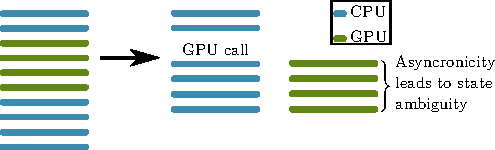
\includegraphics[width=\textwidth]{async.pdf}
	\caption[GPU and CPU asynchronous execution.]{GPU and CPU code run independent of each other. Leads to state ambiguities if both sides need to talk to each other \cite{nvidia}.}
	\label{fig:async_gpu_cpu}
\end{figure}
One of the advantages of GPU-CPU independence is that both can work concurrently on the problem. If both systems have to talk to each other, then one must tread carefully, ensuring proper syncronisation and data mapping before moving (see \cref{fig:async_gpu_cpu}).

The reason why code branching is bad for GPU parallelisation is down to the fact that they work like software customisable vector machines. Where collections of threads all carry out the same operation on different pieces of data at the same time. This means that regardless of whether a condition is true or false, the code will execute. It is only data storage that depends on the condition, as illustrated in \cref{fig:code_branching}.
\begin{figure}
	\centering
	\begin{subfigure}[t]{0.48\textwidth}
		\centering
		\begin{minted}{c}
if (y == 0){
    x = a+b;
}
else if (y == 1){
    x = a*b;
}
else{
    x = a/b;
}
			\end{minted}
		\caption{CPU code will only execute if the condition is met. This is called code branching.}
	\end{subfigure}
	~
	\begin{subfigure}[t]{0.48\textwidth}
		\centering
		\begin{minted}{cuda}
p = (y == 0);
p: x = a+b;

p = (y == 1);
p: x = a*b;


!p: x = a/b;
			\end{minted}
		\vspace{12pt}
		\caption{GPU code executes every line but only stores results if the the flag before the colon is true.}
	\end{subfigure}
	\caption[Explanation of warp divergence.]{The NVidia CUDA compiler replaces \texttt{if} and \texttt{case} statements with logical flags \texttt{p}. Every line is executed, but the data is only stored if the flag prior to the colon is true \cite{nvidia}. This means that having rare but computationally expensive special cases will tank parallel performance and must therefore be dealt with separately.}
	\label{fig:code_branching}
\end{figure}

Dislocation Dynamics (DD)---in particular 3D Discrete Dislocation Dynamics (3D DDD)---can greatly benefit from parallelisation, especially when coupling to Finite Element Methods (FEM). It is worth noting that there are potential issues arising from the very computationally expensive functions and special cases that often arise from analytical solutions in 3D DDD. There are also potential issues with data redundancy---which are non-limiting in the short term---that may eventually require a more data-efficient approach as the computational capabilities and data capabilities of GPUs converge. \Cref{ss:parallel_ddd} expands on these issues in the context of DD.

\section{3D Dislocation Dynamics Modelling}
\label{s:3d_ddd}
The plastic deformation of materials is generally governed by the generation and motion of line defects known as dislocations through the crystal lattice. Microstructural features such as grain boundaries, precipitates and inclusions impede dislocation motion causing strengthening but often limiting ductility \cite{init_fail_dln}. Understanding the behaviour of the dislocation ensemble is highly complicated even when ignoring dislocation-microstructure interactions. However, if we want to truly comprehend their real-world behaviour, we cannot limit ourselves to idealised scenarios.

One of the most often used parametrisations of DD is Discrete Dislocation Dynamics (DDD). Where dislocations are parametrised as a series of nodes linked by straight line segments. This reduces computational requirements and allows for analytic solutions to be obtained. At present, neither DDD or Finite Element (FE) models can truly handle all of the complexities of real-world alloys \cite{ddd_fem1, paradis, fem_ddd2, fem_ddd}. For one, DDD relies on assuming a linear-elastic isotropic solid domain with periodic boundary conditions, while FE relies on assuming continuum properties inside its \emph{finite} domain.

Crystal Plasticity Finite Element Methods (CPFEM) use constitutive equations to calculate dislocation motion and generation on a set of slip systems. These are given as dislocation densities and thus are still ``bulk'' models because they don't interact with each other \cite{cpfem1}. CPFEM can handle finite strains and anisotropy but not strain localisation/slip bands, etc.

Furthermore, dislocations often accumulate in the vicinity of microstructural features. The interaction of dislocations with microstructure can lead to further increased hardening and local hot spots in stress that can lead to failure initiation \cite{size_effects, dln_ind_hard}. Hardware accleration, i.e. using Graphics Processing Units (GPUs), has been shown to be very effective in DDD \cite{gpu_ddd}, and has the potential to enable the simulation of much larger numbers of dislocations for longer timescales. In order to study these phenomena we must find a way of coupling DDD and FEM into a single multiscale model that can simulate micromechanical tests more accurately than CPFEM. With a model such as this we may potentially be able to predict and observe emergent phenomena/properties, explain michromechanical behaviours, and even predict and explain experimental results based on underlying dislocation mechanisms.

\subsection{Coupling Dislocation Dynamics to Finite Element Methods}
\label{ss:ddd_fem}
Coupling dislocation dynamics (DD) to FEM is important to properly simulate micromechanical tests because DD provides us with a more precise set of inputs and greater granularity for solving the FE problem. There are at present two methods with which to do so, the \nameref{sss:superposition} and the \nameref{sss:discrete_continuum}. The most accurate implementation of dislocation dynamics is discrete dislocation dynamics, where the dislocation is broken into nodes and connecting segments. This is compuationally efficient and allows for analytical solutions. However, as discussed in \cref{sss:lvl_set} explicit discretisation is not the only way to tackle the problem.

\subsubsection{Superposition Model}
\label{sss:superposition}
\begin{figure}
	\centering
	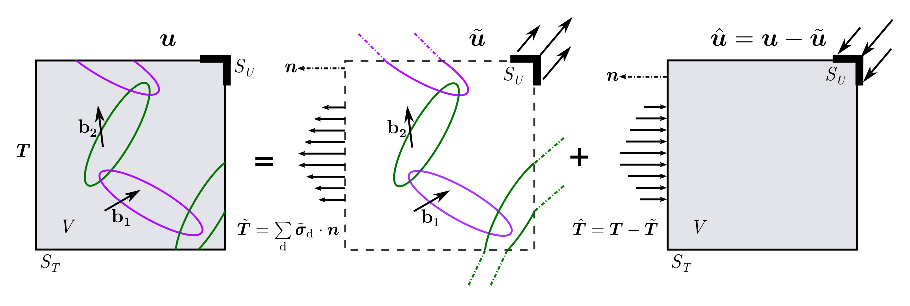
\includegraphics[width=\linewidth]{fem_ddd.eps}
	\caption[Superposition Model for DDD-FEM coupling.]{Decomposition of the boundary value problem. The volume $ V $ is bounded by surface $ S $ contains a dislocation ensemble and is subjected to initial traction conditions $ \vec{T} $ on $ S_{T} $ and $ \vec{u} $ on $ S_{u} $. First, the traction, $ \vec{\tilde{T}} $, and displacement, $\vec{\tilde{u}}$, fields due to the dislocations in the infinite domain (DDD) are evaluated on the boundaries $ S_{T} $ and $ S_{u} $ respectively. Then a traditional FE method is used to calculate the stress field satisfying the boundary conditions $ \vec{\hat{T}} = \vec{T} - \vec{\tilde{T}} $ and $ \vec{\hat{u}} = \vec{u} - \vec{\tilde{u}} $. Image edited from \cite{analytic_tractions}.}
	\label{fig:fem_ddd}
\end{figure}

The Superposition Model (SM) works by decomposing the problem into separate DDD and FE problems (\cref{fig:fem_ddd}). It is assumed that a linear-elastic body $ V $ bounded by a surface $ S $ is subject to traction boundary conditions, $ \vec{T} $, on $ S_{T} $ and displacement boundary conditions, $ \vec{u} $, on $ S_{u} $. The formulation proposed in \cite{dismot} to impose traction-displacement boundary conditions on DDD problems in finite domains states that the total displacement and stress fields can be written as a superposition of displacement and stress fields obtained from DDD and FE,
\begin{subequations}
	\label{eq:superposition}
	\begin{align}
		\vec{u}      & = \vec{\tilde{u}} + \vec{\hat{u}}\,,            \\
		\tns{\sigma} & = \tns{\tilde{\sigma}} + \tns{\hat{\sigma}}\, .
	\end{align}
\end{subequations}
The (\textasciitilde) fields are those associated with the dislocation in an infinite medium and are obtained by evaluating analytic fields in a DDD simulation. While the corrective (\textasciicircum) fields are those which must be superimposed to ensure the boundary conditions are met. This means that the image fields can be obtained by running a FE simulation with the ``corrected'' displacement and traction fields,
\begin{subequations}
	\begin{align}
		\vec{\hat{u}}                    & = \vec{u} - \vec{\tilde{u}}\,,                                                                                 \\
		\tns{\hat{\sigma}} \cdot \vec{n} & = \vec{\hat{T}} = \vec{T} - \underbrace{\vec{\tilde{T}}}_{\displaystyle{\tns{\tilde{\sigma}}}\cdot \vec{n}}\,,
	\end{align}
\end{subequations}
where $ \vec{n} $ is the outer unit normal vector to $ S $. As a dislocation segment moves closer to the surface, its (\textasciitilde) field diverges and starts causing numerical problems \cite{bdd}. A further problem with this method is that modelling elastic inclusions not only requires the calculation of forces induced by dislocations on the inclusion's surface, but also demands the calculation of so-called polarisation stresses due to differences in the inclusion's and matrix properties \cite{dismot, bdd, ddd_precip}.

The relative simplicity of the superposition method has made it a popular choice \cite{analytic_tractions, ddd_fem_sm, ddd_fem_sm2} for coupling DDD and FEM because all it requires is the calculation of forces and displacements on the boundaries (see \cref{ss:analytic_forces}).

\subsubsection{Discrete Continuum Model}
\label{sss:discrete_continuum}
The Discrete Continuum Model (DCM) takes an alternative approach to solving the same problem. The DCM only treats short-range dislocation-dislocation interactions analytically while all other interactions are numerically calculated via FEM \cite{dcm}. It is based on the regularisation of the atomic displacement jump across the slip plane into a plastic strain inclusion according to eigenstrain theory \cite{eigenstrain}. Like the Superposition Model, the DCM also assumes the simulated volume to be linear-elastic.

The eigenstrain formalism assumes that material defects can be represented as stress-free strain distributions dubbed eigenstrains \cite{eigenstrain}. For example, a dislocation loop of any shape may be approximately represented, thin, coherent, plate-like inclusion with the same contour as the loop and a characteristic thickness $ h $ as shown in \cref{fig:eigenstrain} \cite{dcm}. The eigenstrain tensor, $ \epsilon^{\rvar{p}} $, can then be defined as a symmetric dyadic product of the Burgers vector, $ \vec{b} $, and slip plane normal $ \vec{n} $,
\begin{align}\label{eq:eigenstrain}
	\tns{\epsilon^{\rvar{p}}} & \equiv \dfrac{1}{2h} (\vec{b} \otimes \vec{n} + \vec{n} \otimes \vec{b})\,.
\end{align}
\cref{eq:eigenstrain} can be used to calculate approximate elastic fields from the stress-free eigenstrain distribution. The approximation is accurate far from the dislocation core \cite{dln_core}. As we move closer but still outside of the core region, the approximation tends toward the exact discrete dislocation solution as $ h \to 0$. Due to linear elasticity, the total plastic strain is the sum of the individual plastic strains due to each dislocation segment.
\begin{figure}
	\centering
	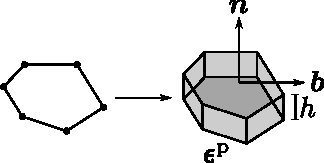
\includegraphics[width=0.5\linewidth]{eigenstrain.pdf}
	\caption[The eigenstrain formalism.]{The eigenstrain formalism as defined in \cite{eigenstrain}. The dislocation is being approximated by a thin coherent inclusion of thickness $ h $, whose strain-free stress tensor $ \tns{\sigma^{\rvar{p}}} $ as defined by \cref{eq:eigenstrain}. The vectors $ \vec{n} $ and $ \vec{b} $ are the normal vector to the slip plane and the dislocation line's Burgers vector.}
	\label{fig:eigenstrain}
\end{figure}

The formalism then lets us solve the boundary value problem by finding the stress tensor $ \tns{\sigma} $, elastic strain $ \tns{\epsilon^{\rvar{e}}} $ and displacement $ \vec{u} $ in mechanical equilibrium with the boundary conditions and plastic strain distribution $ \tns{\epsilon^{\rvar{p}}} $ from the ``inclusions''.

It is worth noting that in order to calculate the eigenstrains, there must be sufficient FE nodes inside the thin plate. Therefore smaller values of $ h $ necessitate finer FE meshes. Furthermore, the original DCM experienced numerical blow up as dislocation-dislocation distances approached $ h $ \cite{dcm0}, but this has since been addressed. Assuming linear-elasticity, the revised model \cite{dcm} yields,
\begin{subequations}\label{eq:discrete_continuum}
	\begin{align}
		\nabla \cdot \tns{\sigma} + \vec{f} = \vec{0} \quad & \in V \setminus \{A\}\,, \\
		\tns{\sigma} = \tns{E} : \tns{\epsilon} \quad       & \in V \setminus \{A\}\,, \\
		[[\vec{u}]] \quad                                   & \rvar{across } \{A\}\,,  \\
		\vec{u} = \vec{u_{0}} \quad                         & \in S_{u}\,,             \\
		\tns{\sigma} \cdot \vec{n} = \vec{T} \quad          & \in S_{T}\,.
	\end{align}
\end{subequations}
At time $ t $, $ \{A\} $ denotes the area swept by the dislocation loops since the start of the simulation. $ [[\vec{u}]] $ denotes displacement jumps tangent to $ \{A\} $ due to dislocation glide; its magnitude and direction depend on the Burgers vector $ \vec{b} $. $ \tns{E} $ is the 4\textsuperscript{th}-order elasticity tensor, $ \tns{\sigma} $ the small strain tensor, $ \vec{f} $ are the body forces and, $ : $, is the double dot product defined as, $ (\tns{E}:\tns{\epsilon})_{ij} = E_{ijkl}\epsilon_{kl} $, for a rank 4 tensor $ \tns{E} $ and rank 2 tensor $ \tns{\epsilon} $. The operator, $ \setminus $, is the set difference defined as, $ A \setminus B = \{x \in A | x \notin B\} $. We use the same notation for the volume, surface normal and boundary conditions as in \cref{sss:superposition}. \cref{eq:discrete_continuum} can then be linearly decomposed three parts which are solved via FEM or DDD and coupled.

It is worth noting that the DCM is substantially more complicated than the SM. By requiring the finite elements be small enough for the eigenstate formalism to work, it strongly couples DDD to the FE model and software. It shifts the brunt of the computational workload from DDD to FEM. Essentially trading computationally intensive long range interactions which scale on the order of $ \mathcal{O}(N^{2}) $, where $ N $ is the number of dislocation line segments; for computationally intensive tasks scaling on the order of $ \mathcal{O}(M^{3}) $ where $ M $ is the number of finite elements in a cubic mesh with $ N $ elements per side. Furthermore, it cannot be used with BE methods as the eigenstrain formalism demands the use of internal elements rather than simply requiring a surface mesh.

That said, the DCM allows for reductions in the computational complexity of certain parts of the problem which would otherwise have to be done via DDD \cite{dcm}; namely long-range dislocation-dislocation or dislocation-surface interactions via an interaction distance cutoff that is only possible with the eigenstrain formulation. Compared to the SM, gains in computational efficiency grow as dislocation density increases with respect to the number of finite elements. Since dislocation-dislocation and dislocation-surface interactions are among the most computationally expensive aspects of DDD, the DCM can reduce the overall computational cost of simulations with large enough dislocation densities.
\subsubsection{Level Set Method}
\label{sss:lvl_set}
%
Even though the level set method has not strictly been used to couple DD to FEM, it has been used to model inclusions \cite{ddd_inclusion_as_force} as described in \cref{sss:inclusions}. This type of dislocation dynamics is fundamentally distinct from DDD because Level Set DD uses arbitrary functions rather than a discretisation approach to represent dislocations lines. The idea is that in 3D, a dislocation $ \gamma(t) $ can be represented by the intersection of two zero levels of two level set functions (see \cref{fig:lvl_set_dd}),
\begin{subequations}\label{eq:lvl_set}
	\begin{align}
		\phi(x(t),y(t),z(t),t)                                                          & = 0\,, & \qquad
		\psi(x(t),y(t),z(t),t)                                                          & = 0\,,          \\
		\dfrac{\rvar{d} \phi}{\rvar{dt}} = \partial_{t}\phi + \vec{v} \cdot \nabla \phi & = 0\,, & \qquad
		\dfrac{\rvar{d} \psi}{\rvar{dt}} = \partial_{t}\psi + \vec{v} \cdot \nabla \psi & = 0\,,
	\end{align}
\end{subequations}
where $ \vec{v} $ is the dislocation velocity. This definition uses the material derivative because it is assumed that the function and its spatial coordinates are all functions of time, $ t $. The material derivative also comes up when deriving the Navier-Stokes equations of fluid dynamics.
\begin{figure}[t]
	\centering
	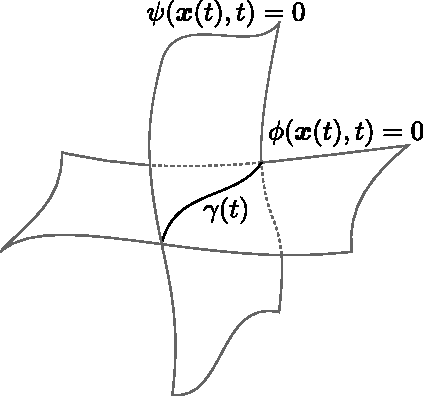
\includegraphics[width=0.3\linewidth]{level_set.pdf}
	\caption[Level set Dislocation Dynamics.]{Diagram of a continuous dislocation $ \gamma(t) $ as the intersection of the zero level of two level set functions $ \phi(\vec{x}(t),t),~\psi(\vec{x}(t),t) $ as posed by \cref{eq:lvl_set}. Image edited from \cite{lvl_set_dd}.}
	\label{fig:lvl_set_dd}
\end{figure}

The level set method is significantly more computationally more expensive than DDD \cite{lvl_set_dd}. It must solve two coupled quasi-linear partial differential equations whose character is in general undefined. It therefore requires the use of very robust numerical solvers such as higher order Total Variation Deminishing (TVD) Runge-Kutta methods for time discretisation (TVD-RK4 or higher) and high order ENO (Essentially Nonoscillatory $ \mathcal{O}(N^5) $ or higher) or WENO (Weighted Essentially Non-Oscilatory) interpolation methods for spatial discretisation \cite{lvl_set_ddd_inc} for the solutions to converge satisfactorily. The method also makes it impossible to obtain many of the useful analytical solutions one can find by discretising dislocations into straight line segments. Another problem is that this method has never been truly coupled to the finite element method. However, if one were to do so there are two naïve ways of going about it:
\begin{inparaenum}[\itshape1\upshape)]
	\item numerically integrating along the dislocation lines and finding a way to numerically calculate the forces on FE nodes, or
	\item discretising the level set curves and using either the DCM or SM to find forces and displacements.
\end{inparaenum}
The former would be very computationally expensive. Furthermore, no one has found a way to compute the forces or displacements exerted by generally shaped, non-discretised dislocations, numerical solutions are possible as they are needed to find self-interaction energies and dislocation-dislocation forces \cite{lvl_set_dd} but general, closed-form analytical ones are most likely impossible to find. The latter defeats the purpose of the level set method by abandoning the continuum framework. As a result of this, the level set method is not nearly as popular as DDD utilising either the SM or DCM.

\subsection{Non-Singular Continuum Theory of Dislocations}
\label{ss:non-singular_dln}
The Peach-Koehler formula describes the fundamental interactions of dislocations \cite{pk_force} according to the force, $ \vec{f} $, that a local stress $ \tns{\sigma} $ exerts on a dislocation line with Burgers vector, $ \vec{b} $, and line direction, $ \vec{\xi} $,
\begin{align}
	\vec{f} & = (\tns{\sigma} \cdot \vec{b}) \times \vec{\xi}\,.
\end{align}

According to \cite{mura_t}, the internal stress field of a dislocation loop in a homogenous, infinite, linear-elastic medium is given by the contour integral around a loop $ L $,
\begin{align}\label{eq:field_stress}
	\sigma_{ij}^{\infty}(\vec{x}) & = C_{ijkl} \oint_{L} \epsilon_{lnh} C_{pqmn} \dfrac{\partial G_{kp}(\vec{x} - \vec{x'})}{\partial x_{q}} b_{m}\; \rvar{d}x'_{h}\,,
\end{align}
where $ C_{ijkl} $ is the elastic stiffness tensor, $ \epsilon_{lnh} $ the permutation operator, $ \vec{b} $ the Burgers vector, and $ G_{kp}(\vec{x} - \vec{x'}) $ is Green's function of elasticity \cite{mura_t}. $ G_{kp}(\vec{x} - \vec{x'}) $ is defined as the displacement component in the $ x_{k} $ direction at point $ \vec{x} $ in response to a unit point force applied in the $ x_{p} $ direction at point $ \vec{x'} $ \cite{a_non-singular_continuum_theory_of_dislocations}. In an isotropic elastic solid, $ G(\vec{x} - \vec{x'}) $, takes the form,
\begin{align}\label{eq:elastic_green_func}
	G_{ij}(\vec{x} - \vec{x'}) & = \dfrac{1}{8\pi \mu}\left[ \delta_{ij} \partial_{pp} - \dfrac{1}{2(1-\nu)} \partial_{ij} \right] R(\vec{x} - \vec{x'})\,,
\end{align}
where $ \mu $, $ \nu $ are the isotropic shear modulus and Poisson's ratio respectively, $ \delta_{ij} $ is the Kronecker Delta, $ \partial_{x_{1} \ldots\, x_{n}} \equiv \dfrac{\partial^{n}}{\partial x_{1} \ldots\, \partial x_{n}}$, and $ R = \lVert \vec{x} - \vec{x'} \rVert $. However considering that $ \vec{x} \to \vec{x'} \Rightarrow R \to 0 \Rightarrow \partial_{i} R \to \infty $, some (or all) components of the stress field diverge. Furthermore, the total elastic energy also diverges,
\begin{align}\label{eq:e_dln1}
	E & = \dfrac{1}{2} \int S_{ijkl} \sigma_{ij}(\vec{x}) \sigma_{kl}(\vec{x})\; \rvar{d}^{3}\vec{x}\,,
\end{align}
where $ S = C^{-1} $ is the elastic compliance tensor. These divergent properties often prove problematic when numerically computing dislocation forces and energies. \Cref{eq:e_dln1} can also be expressed as a double line integral \cite{dewit1, dewit2},
\begin{align}\label{eq:e_dln2}
	E = & - \dfrac{\mu}{8\pi} \oiint_{L} \partial_{k} \partial_{k} R(\vec{x}-\vec{x}') b_{i} b'_{j} \;\rvar{d}x_{i} \;\rvar{d}x'_{j}\nn
	    & - \dfrac{\mu}{4 \pi (1-\nu)} \oiint_{L} \partial_{i} \partial_{j} R(\vec{x}-\vec{x}') b_{i} b'_{j} \;\rvar{d}x_{k} \;\rvar{d}x'_{k}\nn
	    & + \dfrac{\mu}{4 \pi (1-\nu)} \oiint_{L} \partial_{k} \partial_{k} R(\vec{x}-\vec{x}') b_{i} b'_{i} \;\rvar{d}x_{j} \;\rvar{d}x'_{j}\nn
	    & - \nu \oiint_{L} \partial_{k} \partial_{k} R(\vec{x}-\vec{x}') b_{i} b'_{j} \;\rvar{d}x_{j} \;\rvar{d}x'_{i}\;,
\end{align}
which is important when describing how \citet{a_non-singular_continuum_theory_of_dislocations} derived their non-singular expression.

The singularity in $ R $ is the result of unreasonably and unphysically assuming a dislocation loop's Burgers vector distribution is a Delta function. The assumption was made to allow for closed-form and relatively simple expressions. As noted in \cite{bv_dist}, other distributions may be used but they either result in significantly more complicated expressions or destroy the analytical nature of the classical formulation.

There have been many attempts at removing this singularity, including finite-strain elasticity \cite{non_sing3}, non-local and gradient elasticity \cite{non_sing1, non_sing2}, interaction cut-off radius \cite{pk_force}, average stress at two points on opposite sides of the dislocation line \cite{non_sing4, non_sing5}, and spreading the Burgers vector distribution out over a finite width \cite{bv_dist, non_sing6, non_sing7}. Unfortunately all of these approaches failed in one way or another \cite{a_non-singular_continuum_theory_of_dislocations}. Depending on the approach, the following undesirable qualities may present themselves include inconsistencies, impractical implementation, lack of closed-form solutions for non-straight finite dislocations, lack of self-consistency, and the possibility for multiple expressions and solutions for the line integral of the dislocation line energy.

\Citet{a_non-singular_continuum_theory_of_dislocations} took it upon themselves to define and justify a different Burgers vector distribution that maintains the mathematical convenience of the classical formulation that also eliminates such an unphysical assumption. They did so by introducing a Burgers vector density function,
\begin{subequations}\label{eq:b_dist}
	\begin{align}
		\vec{b}          & = \int \vec{g}(\vec{x}) \;\rvar{d}^{3} \vec{x}\label{seq:bv_dist}\,, \\
		\vec{g}(\vec{x}) & = \vec{b} \tilde{w}(\vec{x}) = \vec{b} \tilde{w}(r)\,,
	\end{align}
\end{subequations}
where $ r \equiv \lVert \vec{x} \rVert $. When substituting \cref{seq:bv_dist} into \cref{eq:field_stress,eq:e_dln2} the result of multiplying $ R $ with components of $ \vec{b} $ results in the following integrals,
\begin{subequations}\label{eq:r_times_b_dist}
	\begin{align}
		R(\vec{x} - \vec{x}') b_{m}        & = \int R(\vec{x} - \vec{x}'') g_{m}(\vec{x}'' - \vec{x}') \;\rvar{d}^{3}\vec{x}''\,,                                                          \\
		R(\vec{x} - \vec{x}') b_{m} b'_{n} & = \iint R(\vec{x}'' - \vec{x}''') g_{m}(\vec{x} - \vec{x}'') g_{n}(\vec{x}''' - \vec{x}') \;\rvar{d}^{3}\vec{x}'' \;\rvar{d}^{3}\vec{x}'''\,.
	\end{align}
\end{subequations}
Using \cref{eq:b_dist,eq:r_times_b_dist} as guidelines, they defined a the following convolutions,
\begin{subequations}
	\begin{align}
		w(\vec{x}) & \equiv \tilde{w}(\vec{x}) * \tilde{w}(\vec{x}) = \int \tilde{w}(\vec{x}-\vec{x}')\tilde{w}(\vec{x}')\; \rvar{d}^{3} \vec{x}'\,, \\
		R_{a}      & \equiv R(\vec{x}) * w(\vec{x}) = \int R(\vec{x} - \vec{x}') w(\vec{x}') \;\rvar{d}^{3} \vec{x}'\,.
	\end{align}
\end{subequations}
At which point they assumed there exists an integrable function $ w(\vec{x}) $ such that
\begin{align}
	R_{a} = \sqrt{R(\vec{x})^{2} + a^{2}} = \sqrt{x^{2} + y^{2} + z^{2} + a^{2}}\,,
\end{align}
where $ a $ is an arbitrary constant meant to represent the dislocation core radius whose value may be estimated from atomistic simulations. This is essentially a definition that can be used to replace $ R $ in the classical equations and eliminate the singularity by including a free parameter. However, in order to ensure this is mathematically sound, there must indeed exist a function which yields $ R_{a} $ as \citet{a_non-singular_continuum_theory_of_dislocations} defined it. This can be done by making use of the following property for the convolution of two suitably differentiable functions, $ \partial_{i} (f*g) = \partial_{i}f * g = f * \partial_{i} g $. We may take the Laplacian twice,
\begin{subequations}
	\begin{align}
		\nabla^{2}[\nabla^{2} \{R(\vec{x}) * w(\vec{x})\} ] & = \nabla^{2}[\nabla^{2} R_{a}(\vec{x})]\,,                                                             \\
		\nabla^{2}[\nabla^{2} \{R(\vec{x})\}] * w(\vec{x})  & = \nabla^{2}[\nabla^{2} R_{a}(\vec{x})]\,,                                                             \\
		\nabla^{2}[\nabla^{2} \{R(\vec{x})\}]               & = \nabla^{2}\left[\dfrac{2}{R}\right] = -8\pi \delta^{3}(\vec{x}) \label{eq:hand_wavy}\,,              \\
		\nabla^{2}[\nabla^{2} R_{a}(\vec{x})]               & = \nabla^{2}\left[\dfrac{2}{R_{a}} + \dfrac{a^{2}}{R_{a}^{3}}\right] = -\dfrac{15 a^{4}}{R_{a}^{7}}\,, \\
		w(\vec{x})                                          & = \dfrac{15 a^{4}}{8\pi R_{a}^{7}} \label{eq:dist}\,.
	\end{align}
\end{subequations}
\Cref{eq:hand_wavy} is a very brave, handwavy statement given that,
\begin{align}
	\nabla^{2} \left[R^{-1}\right]= \nabla^{2}\left[(x^{2} + y^{2} + z^{2})^{-1/2}\right] = 0\,,
\end{align}
but may be physically ``justified'' by pretending $ \nabla^{2}\left[R^{-1}\right] $ defines a spherical surface of radius 0. And \cref{eq:dist} is a similarly handwavy statement that can be ``justified'' by noting that,
\begin{align}
	\lim\limits_{a\to 0} w(\vec{x}) = \delta^{3}(\vec{x})\,.
\end{align}
Nevertheless, the non-singular formulation by \citet{a_non-singular_continuum_theory_of_dislocations} fixes the physically and mathematically problematic assumption that Burgers vectors follow 3D Dirac delta distributions, and proves useful in producing analytical expressions (see \cref{ss:analytic_forces}) that are not much more complex than the singular case.

\subsection{Analytical Forces Exerted by a Dislocation Line Segment on Surface Elements}
\label{ss:analytic_forces}
Whether using the SM or DCM, coupling DDD to FEM requires the traction field $ \tns{\sigma^{\infty}}(\vec{x}) \cdot \vec{n}(\vec{x}) $ to be distributed among the set of relevant discrete nodes of a FE or BE model. In the DCM model this applies to dislocations that are sufficiently close to the boundary; while in the SM, it applies to all dislocations.
Regardless of the coupling model, the force exerted by a dislocation ensemble on a node $ n $ on element $ e $ is given by,
\begin{align}\label{eq:ddd_fem_force_intro}
	\vec{F}^{(n)} = \int_{S_{e}} \left[\tns{\sigma^{\infty}}(\vec{x}) \cdot \vec{n}(\vec{x})\right] N_{n}(\vec{x})\; \rvar{d}S_{e}\,,
\end{align}
where $ \rvar{d}S_{e} $ is the infinitesimal surface element with surface area $ S_{e} $. $ N_{n}(\vec{x}) $ are so-called shape functions (interpolation functions) that distribute the traction field among the surface element's nodes.

The problematic singularity associated with the classical Volterra dislocation is avoided by using the non-singular formulation of \citet{a_non-singular_continuum_theory_of_dislocations} discussed in \cref{ss:non-singular_dln}, which changes \cref{eq:elastic_green_func} into \cref{eq:ns_elastic_green_func},
\begin{align}\label{eq:ns_elastic_green_func}
	G_{ij}(\vec{x} - \vec{x'}) & = \dfrac{1}{8\pi \mu}\left[ \delta_{ij} \partial_{pp} - \dfrac{1}{2(1-\nu)} \partial_{ij} \right] R_{a}(\vec{x} - \vec{x'})\,.
\end{align}

Using the non-singular definition of $ G(\vec{x}-\vec{x}') $ in \cref{eq:field_stress} we obtain the expression for the stress field of a single straight dislocation line segment bounded by two dislocation nodes (1, 2) \cite{a_non-singular_continuum_theory_of_dislocations},
\begin{align}\label{eq:two_node_stress_field}
	\tns{\sigma}^{(12)}(\vec{x}) =
	 & -\dfrac{\mu}{8\pi} \int\limits_{\vec{x_{1}}}^{\vec{x_{2}}} \left( \dfrac{2}{R_{a}^{3}} + \dfrac{3 a^{2}}{R_{a}^{5}} \right) \left[ \left( \vec{R} \times \vec{b} \right) \otimes \rvar{d}\vec{x'} + \rvar{d}\vec{x'} \otimes \left( \vec{R} \times \vec{b} \right) \right]\nn
	%
	 & + \dfrac{\mu}{4\pi (1 - \nu)} \int\limits_{\vec{x_{1}}}^{\vec{x_{2}}} \left( \dfrac{1}{R_{a}^{3}} + \dfrac{3 a^{2}}{R_{a}^{5}} \right) \left[ \left(\vec{R} \times \vec{b}\right)\cdot \rvar{d}\vec{x'} \right] \mtx{I}_{2}\nn
	%
	 & - \dfrac{\mu}{4\pi (1 - \nu)} \int\limits_{\vec{x_{1}}}^{\vec{x_{2}}} \dfrac{1}{R_{a}^{3}} \left[ \left(\vec{b} \times \rvar{d}\vec{x'}\right) \otimes \vec{R} + \vec{R} \otimes \left(\vec{b} \times \rvar{d}\vec{x'}\right) \right]\nn
	 & + \dfrac{\mu}{4\pi (1 - \nu)} \int\limits_{\vec{x_{1}}}^{\vec{x_{2}}} \dfrac{3}{R_{a}^{5}} \left[ \left( \vec{R} \times \vec{b} \right) \cdot \rvar{d}\vec{x'} \right]\vec{R} \otimes \vec{R}\,,
\end{align}
Substituting \cref{eq:two_node_stress_field} into \cref{eq:ddd_fem_force_intro} yields as many integrals as there are surface nodes. Their exact form depends on the shape functions used. The specifics are out of the scope of this work. For a rectangular surface element, the vector formulation can be converted into a set of local scalar coordinates via a series of scalar projections of the set of basis vectors via \cref{eq:ana_loc_coo},
\begin{align}\label{eq:ana_loc_coo}
	\vec{R}          & = \vec{x} - \vec{x'} = y\vec{t} + r\vec{p} + s\vec{q}\,,                                        & \qquad
	R_{a}            & = \sqrt{\vec{R} \cdot \vec{R} + a^{2}}\,, \nn
	\vec{n}          & = \vec{p} \times \vec{q}\,,                                                                     & \qquad
	y                & = \dfrac{\vec{R} \cdot \vec{n}}{\vec{t} \cdot \vec{n}}\,,                                                \\
	r                & = \dfrac{\vec{R} \cdot (\vec{q} \times \vec{t})}{\vec{p} \cdot (\vec{q} \times \vec{t})}\,,     & \qquad
	s                & = \dfrac{\vec{R} \cdot (\vec{p} \times \vec{t})}{\vec{q} \cdot (\vec{p} \times \vec{t})}\,, \nn
	\rvar{d}\vec{x}' & = -\vec{t} \;\rvar{d}y \nonumber\,,
\end{align}
where $ \vec{n},~\vec{p},~\vec{q},~\vec{t} $ are basis vectors\footnote{Unitary vectors that define a space. This space is not orthogonal because in general only $ \vec{p} \perp \vec{q} $, $ \vec{n} \perp \vec{p} $ and $ \vec{n} \perp \vec{q} $.} that respectively correspond to the outside surface normal of the surface element, the two orthogonal vectors that define the sides of the rectangular surface element, and the dislocation line direction. The integral bounds can then be set up accordingly.

Noting that $ \vec{n} \equiv \vec{p} \times \vec{q} $ is normal to the surface element, if $ \vec{t} $ is parallel to the surface element i.e. a linear combination of $ \vec{p},~\vec{q} $ then the product $ \vec{t} \cdot \vec{n} = 0 $, so this formulation is problematic when a dislocation line segment is parallel to a surface. An easy workaround is to slightly around the axis defined by $ \vec{t} \times \vec{n} $ using the line's midpoint as a fulcrum. This works well in serial code but is problematic for parallelisation due to warp divergence (see \cref{ss:parallel_ddd}).

\Cref{fig:flrs} diagramatically shows the definition of the four basis vectors and summarises the line integrals needed to find an analytical expression of the nodal force.
\begin{figure}[t]
	\centering
	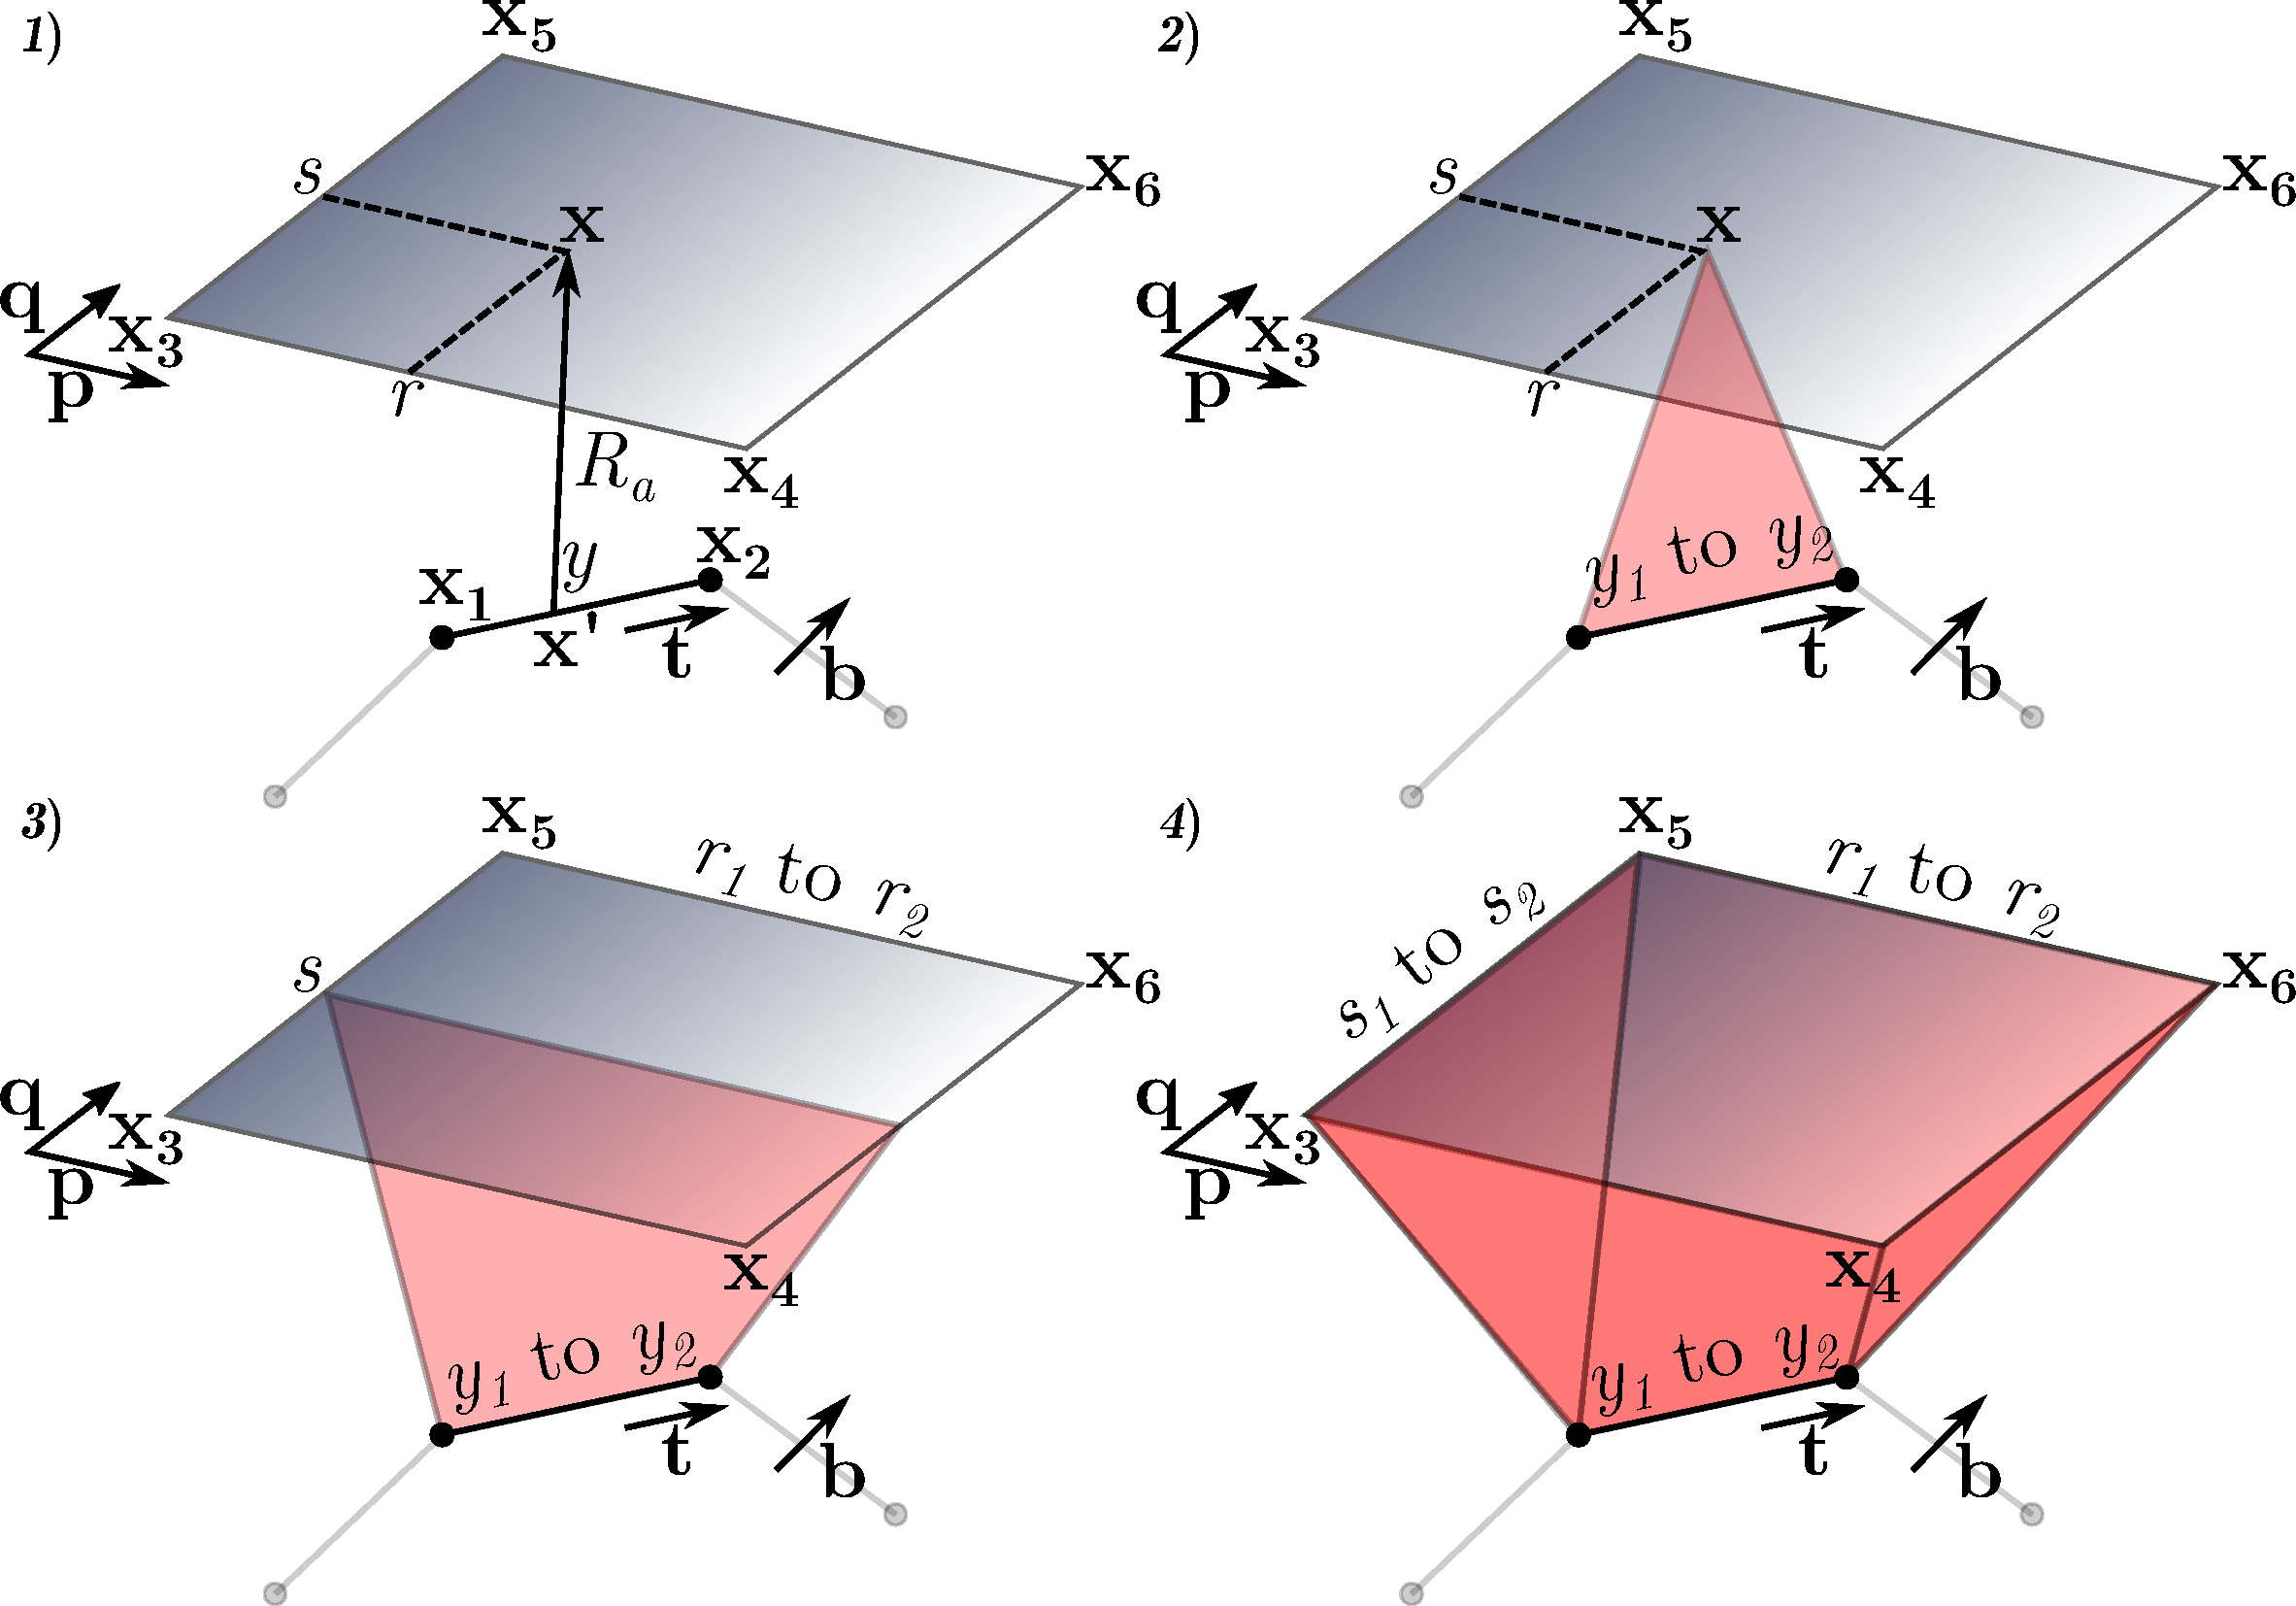
\includegraphics[width=0.8\linewidth]{force_calc_linear_rectangle.pdf}
	\caption[Analytic tractions on linear rectangular surface elements.]{Diagram of the line integral method used to find analytical expressions for the forces exerted by dislocation on linear rectangular surface elements \cite{analytic_tractions}.
		\textit{1}) For any given point $ \vec{x} $ on the surface element and any given point $ \vec{x'}$ on the dislocation line segment, define distance $ R_{a} $.
		\textit{2}) Integrate from $ x_{1} \to x_{2} $ along line direction $ \vec{t} $.
		\textit{3}) Integrate from $ r_{1} \to r_{2} $ along vector $ \vec{p} $.
		\textit{4}) Integrate from $ s_{1} \to s_{2} $ along vector $ \vec{q} $.}
	\label{fig:flrs}
\end{figure}
It is worth noting that over 40 triple integrals arise from \cref{eq:two_node_stress_field,eq:ana_loc_coo}. These were solved via three families of recurrence relationships found via integration by parts and six seed functions found by direct integration. A more detailed description can be found in \cite{analytic_tractions}.

Quadratic triangular surface elements pose a much more challenging problem due to the fact that $ \vec{p} \not\perp \vec{q} $. This property is not the only addition that significantly complicates the integrals, the interpolation functions are quadratic which increase the number of integrals. The non-orthogonality of $ \vec{q},~ \vec{p} $ means the integration limits in the $ r,~s $ coordinates must be parametrised appropriately and the integrations should be carried out in an order suitable for the chosen parametrisation. Aside from these technical considerations, the techniques for solving the problem for quadratic rectangular surface elements are the same as the linear rectangular case \cite{analytic_tractions}. It is worth noting however, that the implementation of such a procedure may require quadruple precision arithmetic.

\subsection{Multiphase Simulations}
\label{ss:multiphase}
%
Modelling heterogeneity in DDD remains challenging. The core assumption of DDD is that we have a homogenous linear elastic space with invariant properties. However, modelling multiphase systems such as multicrystals and inclusions necessitates a weakening of such assumptions, particularly the space's homogeneity. Multiphase models are also necessary to apply DDD to more realistic scenarios.

Fusion in particular is riddled with examples of highly heterogenous materials. As previously mentioned, neutron bombardment often causes clustering of transmutation products particularly on divertor and first wall materials; such clusters often substantially change many of their mechanical and thermal properties. The whole point of Oxide-Dispersion Strengthened (ODS) steels \cite{ddd_ods} is to hamper radiation damage by distributing oxide inclusions within their matrix. If we hope to model such alloys with DDD we must find a way to relax our homogeneity criteria.

Furthermore, many potential candidates for structural and even first wall materials of fusion reactors are designed with complex microstructures in order to resist thermal creep and radiation damage. Understanding dislocation behaviours near the crystal boundaries of these microstructurally complex materials is another niche where DDD simulations can shed light into the mechanisms that give rise to these materials' desirable properties.

\subsubsection{Polycrystalline Materials}
\label{ss:polycrystal}
Polycrystalline materials have been studied using DDD, however most of these are in 2D. One of the easiest phenomena to investigate with 2D DDD are grain size effects \cite{2d_pcm, 2d_pcm2}.

It is well known that much of the grain size strengthening effects arise from dislocation-grain boundary (GB) interactions including transmission, reflection, emission and absorption of dislocations \cite{grain_size_eff1, grain_size_eff2}; with transmission being the most typically observed.

The model depends on the grain boundary energy density, $ E_{\rvar{GB}}(\delta\theta) $, where $ \delta\theta $ is the crystallographic misorientation between neighbouring crystals; resolved shear stress, $ \tau $, on the incoming dislocation with Burgers vector $ \vec{b_{1}} $; critical penetration stress for the GB, $ \tau_{\rvar{GB}} $; and Burgers vector of the dislocation debris, $ \vec{\Delta b} = \vec{b_{1}} - \vec{b_{2}} $, left behind when the incoming dislocation, $ \vec{b_{1}} $, transmits throught the grain boundary to become a dislocation with Burgers vector, $ \vec{b_{2}} $. The relationship may be approximated by,
\begin{align}\label{eq:dln_trns}
	\tau \lvert\vec{b_{1}}\rvert^{2} & \geq \tau_{\rvar{pass}} \lvert\vec{b_{1}}\rvert^{2} = E_{\rvar{GB}}(\theta) \lvert\vec{b_{1}}\rvert + \alpha G \lvert\vec{\Delta b}\rvert^{2}\,,
\end{align}
where $ \alpha $ is the material constant and $ G $ the shear modulus. The grain boundary energy density was proposed by \cite{gb_e_dens} to have the simple form,
\begin{align}
	E_{\rvar{GB}} & = 	\begin{cases}
		k \dfrac{\delta\theta}{\theta_{1}}                 & \quad 0 \leq \delta\theta < \theta_{1}\,,          \\
		k                                                  & \quad \theta_{1} \leq \delta\theta < \theta_{2}\,, \\
		k \dfrac{\pi/2 - \delta\theta}{\pi/2 - \theta_{2}} & \quad \theta_{2} \leq \delta\theta < \pi/2\,,
	\end{cases}
\end{align}
where $ k,~ \theta_{1},~\theta_{2} $, are material specific.

This is of course a gross simplification of the real 3D problem, but this approach was used by \citet{2d_pcm} to investigate the Hall-Petch effect, which correlates grain size with flow stress of a polycrystal,
\begin{align}\label{eq:hall_petch}
	\sigma & = \sigma_{0} + \kappa \left(\dfrac{d_{0}}{d}\right)^{n}\,,
\end{align}
where $ \sigma_{0} $ is the yield stress, $ d_{0} $ a reference crystal size, $ \kappa $ the Hall-Petch slope and $ n $ the crystal size sensitivity parameter. \Citet{2d_pcm} showed that the model reproduces the Hall-Petch effect quite successfully. As a consequence, they showed that even what might appear as an overly simplistic approach can describe a complex emergent phenomenon such as the Hall-Petch effect.

Aside from the Hall-Petch effect, the model has also been utilised by \cite{2d_pcm2} to study the thickness effects of three different types of polycrystalline thin films:
\begin{inparaenum}[\itshape 1\upshape )]
	\item no surface treatment,
	\item surface passivation layer and
	\item surface grain refinement zones
\end{inparaenum}. In this study, Frank-Reed sources were seeded across the domain, and the superposition principle was utilised to calculate displacement, strain and stresses in the thin films. Their results qualitatively reproduced experimental observations from expected dislocation patterns, stress distributions, and the eventual disappearance of the size effect as the films got thicker \cite{2d_pcm2}.

Two-dimensional models might seem useless but they have their place, particularly when thin films are concerned. However, they may also be of use when investigating the effects of dislocations on the mechanical behaviour of superconducting tape---whose applications range from medical imaging to fusion energy production. The exotic composition and crystallography of many superconductors (perovskites) would make 3D models very complex and computationally expensive, so 2D models may offer viable alternatives. On top of this, a superconducting tape's operating environment would often have it under strains which might not strictly lie in-plane, but given a small enough segment of tape, strains orthogonal to the its plane may be neglected. Thus making 2D models an acceptable first attempt at tacking the problem, at leas before computational resources and developments in 3D models make more realistic studies of such complex systems possible.

The 3D case is substantially more complicated than the 2D case. A recent study by \citet{twinning} looked at the role of twinning on the hardening response of polycrystalline Mg using 3D DDD.

The article is a perfect example of why 3D DDD is so much more complex than 2D DDD. Admitedly, it uses a material with a HCP crystal structure which complicates matters compared to FCC or BCC.

In 3D DDD one must account for dislocation-twin boundary (TB) interactions. These may be obtained via geometric considerations, MD, and experimental evidence \cite{twinning2,twinning3,twinning4,twinning5}. We must have information regarding how dislocations are transmitted through a TB such as
\begin{inparaenum}[\itshape 1\upshape)]
	\item whether a dislocation leaves a residual dislocation on the TB,
	\item the possible pre-TB and post-TB slip planes a dislocation can be transmitted to,
	\item which loading conditions are conducive to which transmission behaviour and
	\item which types of dislocation can be transmitted or reflected and in what ways \cite{twinning}.
\end{inparaenum}
All this obviously depends on the twinning plane, so in order to study more realistic scenarios one must have all the necessary knowledge to properly account for all dislocation-TB interactions. Furthermore, it is possible that certain dislocations may leave behind twinning dislocations that end up as TB steps, whose movement can lead to TB migration and twin growth \cite{twinning6, twinning7}.

\Citet{twinning} modelled four scenarios in order to deconvolute the effects that twins and grain boundaries have on the mechanical behaviour of a cubic crystal. They modelled
\begin{inparaenum}[\itshape 1\upshape)]
	\item a cubic twinned polycrustal with two TBs and GBs on the edges of the cube,
	\item a single crystal with no TBs or GBs,
	\item a polycrystal with no TBs but GBs,
	\item a twinned crystal with TBs but not GBs.
\end{inparaenum}
It is worth noting that the effects of twin growth in plasticity were not accounted for in their DDD simulation and instead had to be numerically computed via the hardening rate $ \theta $,
\begin{subequations}
	\begin{align}
		\theta             & = \dfrac{\rvar{d}\sigma}{\rvar{d}\epsilon} = \dfrac{\rvar{d}}{\rvar{d}\epsilon}  \left[E\left(\epsilon - \epsilon_{\rvar{slip}}^{\rvar{p}} - \epsilon_{\rvar{twin}}^{\rvar{p}}\right)\right] = \theta_{\rvar{s}} + \theta_{\rvar{TG}}\,, \\
		\theta_{\rvar{TG}} & = -\dfrac{\rvar{d}}{\rvar{d}\epsilon} \left[E \epsilon_{\rvar{twin}}^{\rvar{p}} \right] = -E \bar{m} \gamma_{\rvar{twin}} \dfrac{\rvar{d}}{\rvar{d} \epsilon} \left[f_{\rvar{twin}}\right]\label{seq:tg}\,,
	\end{align}
\end{subequations}
where $ \theta_{\rvar{TG}} $ is the hardening rate due to twin growth, $ \bar{m} $ the mean Schmid factor of the participating twins $ \gamma_{\rvar{twin}} $ the characteristic twinning shear and $ \dfrac{\rvar{d}}{\rvar{d} \epsilon} \left[f_{\rvar{twin}}\right] $ is the change in the change in the twin volume fraction with respect to applied strain. These parameters must be empirically obtained.

With their model, \citet{twinning} managed to qualitatively reproduce experimental observations, including the concave shape of strain-stress curves that arises from the competing hardening effect of TBs restricting dislocation motion (\cref{fig:twinning}), and the softening produced by twin growth as obtained from \cref{seq:tg}.
\begin{figure}[t]
	\centering
	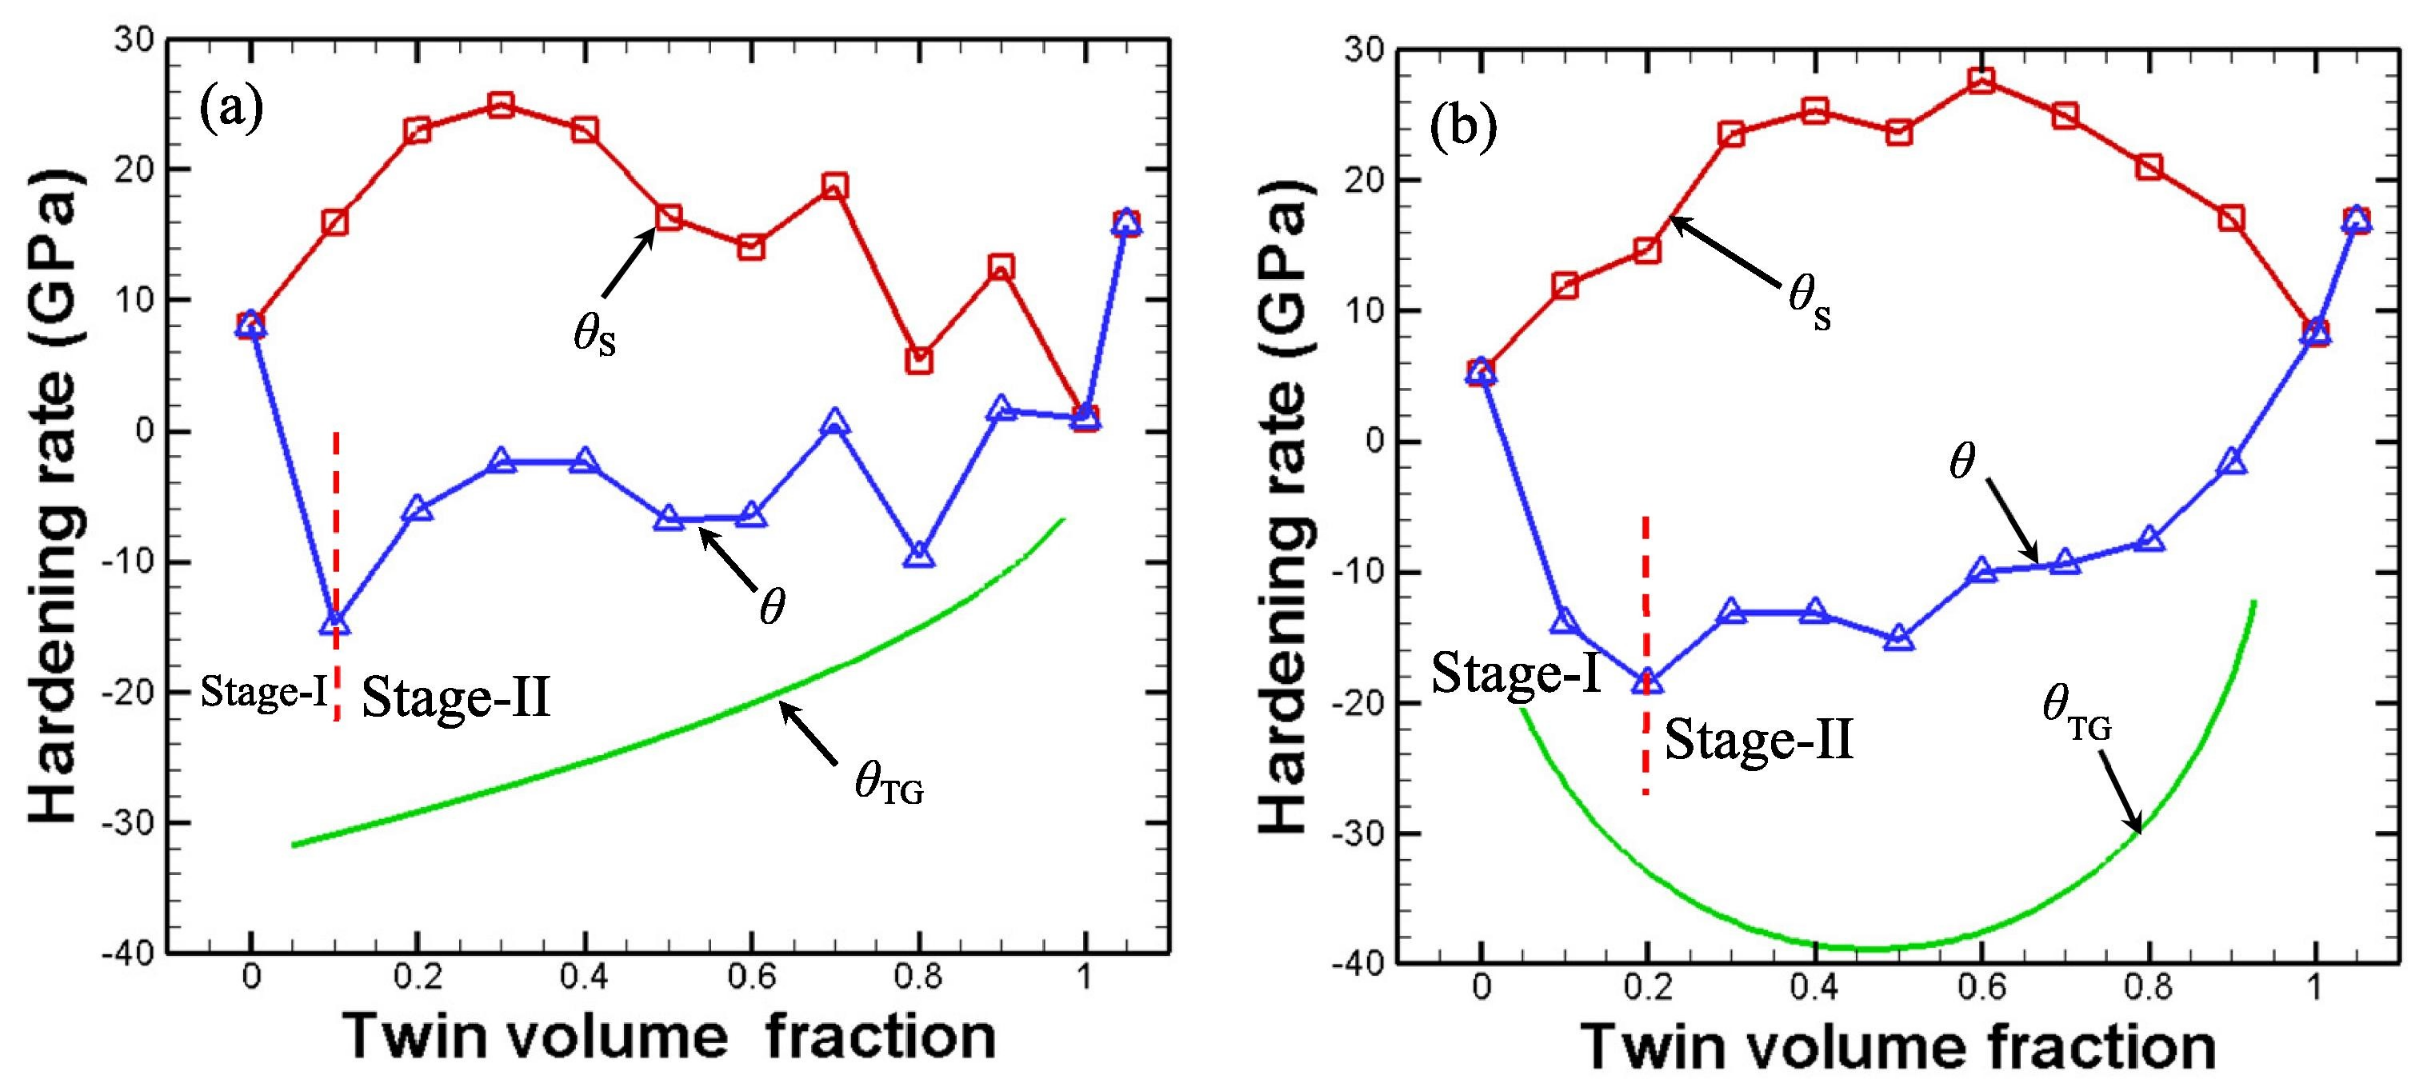
\includegraphics[width=\linewidth]{twinning.png}
	\caption[Modelling twinned multicrystals with DDD.]{Simulated hardening rate as a function of twin volume fraction for (a) yz compressive loading and (b) tensile loading. Image edited from \cite{twinning}.}
	\label{fig:twinning}
\end{figure}

Twin boundaries in 3D are analogous to grain boundaries in 2D, given that they are coherent, narrow boundaries rather than messy, often incoherent grain boundaries. Consequently, grain boundaries are much harder to treat in 3D; instead, the community focuses on multiphase models where the details of dislocation transmission between phases are ignored or simplified as mentioned in \cref{sss:inclusions}.

\subsubsection{Inclusions}
\label{sss:inclusions}
Inclusions have been modelled using the three methods described in \cref{ss:ddd_fem}. However, they have gone about it differently. The SM and DCM apply their formulations heirarchically to allow for dislocation motion into and out of the inclusion. Furthermore, being coupled DDD-FEM problems, the inclusions must also be appropriately meshed, oftentimes this means inclusion geometries are limited to the mesh type. However, FEM allows for the calculation of coherency stresses which are seen by the dislocations and cause dislocation localisation and forresting in the vicinity of inclusions, just as experimentally observed \cite{sm_incl, dcm_incl}.

The level set method, having never been coupled to FEM, takes a different approach. Where the particles can be modelled as a region where dislocations experience a user-defined force. Coherency stresses have so far been neglected, but their effects may be modelled with the use of functions akin to diffuse orbital functions used in theoretical and computational quantum chemistry. Within this framework the inclusions may be arbitrarily defined to have any smooth shape, especially if one were to use piecewise parametric fourier curves.

Dislocation-permeable inclusions have been simulated via the SM \cite{sm_incl}. As mentioned in \cref{sss:superposition}, there is a need to calculate polarisation stresses due to differences in the elasticity of both phases. Using the same notation as \cref{sss:superposition} this can be done by breaking up the image stress into,
\begin{subequations}
	\begin{align}\label{eq:sm_pol_stress}
		\tns{\hat{\sigma}} & = \tns{^{\rvar{m}}C} \tns{\hat{\epsilon}} \quad \in V_{\rvar{m}}                                                                                  \\
		\tns{\hat{\sigma}} & = \tns{^{\rvar{p}}C} \tns{\hat{\epsilon}} + \left[\tns{^{\rvar{p}}C} - \tns{^{\rvar{m}}C}\right] \tns{\tilde{\epsilon}} \quad \in V_{\rvar{p}}\,,
	\end{align}
\end{subequations}
where $ \rvar{m},~\rvar{p} $ denote whether a variable belongs to the matrix or precipitate respectively and $ \tns{C} $ is the elastic stiffness tensor.

\Citet{sm_incl} not only modelled a cuboid inclusion, but bimetallic interfaces in 3D. They found that under the right conditions, dislocations can pass from one phase to the other. When a dislocation passes into a different phase, it leaves an antiphase boundary on the slip plane. Therefore, in order for a dislocation to move from one phase to another, it needs excess energy equal to the antiphase (APB) energy of the area it sweeps within the precipitate. This means that as a node passes from one phase to another, it feels a repulsive force $ F_{b} $. The next dislocation moving along the same APB will then feel an attractive force $ F_{b} $ to dissolve the APB. Once both dislocations move into the new matrix, they form a superdislocation bound by the APB energy \cite{apb}. However, as the dislocation length increases with respect to the precipitate's volume, the production of Orowan loops around it becomes more energetically favourable than moving into the new phase \cite{sm_incl, apb}. Both of these behaviours have been observed when using the superposition method.

The eigenstrain method \cite{eigenstrain_incl} as described in \cref{sss:discrete_continuum} has been shown to be a viable solution to this problem. One can compute the stresses and displacements produced by the dislocation ensemble on the inclusions' surfaces via DCM or SM. The SM method however needs to calculate polarisation stresses \cite{bdd}, an operation that significantly increases the number of calculations necessary to solve the problem.

The DCM method has been used to simulate multiphase materials where the simulated dislocations reproduced experimentally observed behaviours such as the zig-zag patterns and dislocation forests produced by dislocations around precipitates in nickel superalloys \cite{dcm0, dcm_incl}. Reproducing such behaviours is not as trivial as simply adding inclusions to the simulation domain. In order to produce accurate results, one requires knowledge of the coherency stress between the different phases \cite{dcm_incl}. Such stresses are often due to lattice mismatches and differences in the thermal expansion coefficients. These coherency stresses localise the dislocations around the inclusions and are responsible for the observed localisation and aggregation of dislocations around precipitates as seen in \cref{fig:coherency} \cite{dcm_incl}.
\begin{figure}[t]
	\centering
	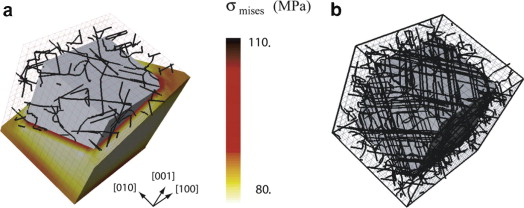
\includegraphics[width=\linewidth]{dln_inclusion.jpg}
	\caption[Modelling dislocation inclusion interactions with the discrete continuum model.]{(a) Shows the initial dislocation configuration after relaxation in the presence of the calculated von Mises coherency stresses $ \tns{\sigma}_{\rvar{mises}} $. (b) Shows the dislocation forresting around the inclusion as a result of 0.2\% plastic strain for the [001] case. Image obtained from \cite{dcm_incl}.}
	\label{fig:coherency}
\end{figure}

The level set method has also been successfully used to model inclusions. In contrast to the aforementioned methods, they are assumed to be regions in space where dislocations experience a repelling force, instead of a region in space with distinct characteristics to the matrix. The force profile can be very simply defined to depend on the radial distance from the dislocation to a point in the ``inclusion's'' volume \cite{ddd_inclusion_as_force}. It can also be modulated depending on the nature of the inclusion by making the force a radial function, thus avoiding many of the numerical issues facing DDD-FEM couplings (see \cref{ss:ddd_fem,ss:analytic_forces}). It is also possible to make the inclusions impermeable or semi-permeable depending on the magnitude and steepness of the force gradient as presented in \cite{ddd_inclusion_as_force}. Arbitrarily shaped may also be possible if one were to also use angular components to the force function, or even through the use of spherical harmonics.

Though mathematically appealing, the level set method is far from representing the reality of dislocation-inclusion interactions. More realistic scenarios require use of more commonplace DDD-FEM coupling methods. Implementing arbitrarily shaped particles is not impossible in DDD---particularly if they can be discretised. Aside from the significantly lower computational requirements, one of the biggest advantages of DDD is that one can find tractions and displacements natively through either the DCM or SM, whereas the level set method requires the force to be user-defined and displacements on the inclusion are completely ignored. Furthermore, if the inclusion is a different crystal or a twin of the same material as in \cite{twinning}, it is possible to use the DCM or SM to study the transmission of dislocations from one phase to the other; something that is not yet possible to do with the level set method.

\subsection{Parallelising Discrete Dislocation Dynamics}
\label{ss:parallel_ddd}
It has been shown that DDD lends itself well to parallelisation. \Citet{gpu_ddd} investigated some of the more computationally intensive parts of DDD in DDLab \cite{ddlab}, a freely available DD code for Matlab. The algorithms whose parallel performance was studied in \cite{gpu_ddd} were
\begin{inparaenum}
	\item segment-segment interaction,
	\item surface tractions and
	\item image stresses.
\end{inparaenum}

The segment-segment interaction has $ \mathcal{O}(N^{2}) $ computational complexity, where $ N $ is the number of dislocation segments. The quadratic scaling is due to the $ r^{-1} $ dependence of the dislocation stress fields, so long range interactions cannot be ignored.

Both the surface traction and image stress calculations have $ \mathcal{O}(k N) $ computational where $ k $ is the total number of surface nodes and $ N $ the number of dislocation line segments.

As is usually the case in parallel computing, there is often more than one way to parallelise a problem. The optimal strategy depends on the problem itself. It was no different in \cite{gpu_ddd} as shown in \cref{fig:gpu_ddd}. \Citet{gpu_ddd} realised that the segment-segment interaction calculation can be done via $ \mathcal{O}(N^{2}) $ parallelism, where single pairs of dislocation segments are sent to a single thread, and then globally reduced. However this approach requires $ \mathcal{O}(N^{2}) $ memory and can lead to inefficient data reuse. So they opted instead for $ \mathcal{O}(N) $ parallelisation and serialisation. In this scheme each thread is assigned a unique segment, and each thread computes the forces between its assigned segment and all the others while serially adding the force contributions. The memory access pattern they found best was that of a serial procedure, the reason is that in-thread calculations are serialised so having coalesced memory access patterns for threads would cause problems when serially accessing data for the calculation.
\begin{figure}[t]
	\centering
	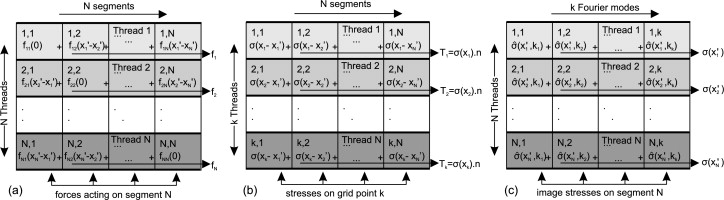
\includegraphics[width=\linewidth]{gpu_ddd.jpg}
	\caption[Parallelisation strategies for three problems in 3D DDD.]{Parallelisation strategies for: (a) the $ N^{2} $ segment interactions; (b) surface traction at k grid points and; (c) and image stresses on $ N $ segments. Image taken from \cite{gpu_ddd}.}
	\label{fig:gpu_ddd}
\end{figure}

However, there is another approach \citet{gpu_ddd} did not consider. It combines both of the aforementioned strategies, $ \mathcal{O}(N^{2}) $ memory and $ \mathcal{O}(N) $ parallelisation and serialisation. Such an approach requires two copies of the input data (one per access pattern). One pattern would allow each thread to obtain its uniquely assigned segment in a coalesced manner. The second would be the serial access pattern already present. Thus obtaining the best performance possible performance at the cost of doubling the required memory. This is a better strategy provided there is enough device memory\footnote{Assuming the line direction is calculated inside the program, each dislocation line segment represents 3, 3-element vectors of type double (8-bytes per entry), totalling 72 bytes in global memory per dislocation line segment (two nodes + Burgers vector per segment). There must also be enough global memory to output the forces, which represent 1, 3-element vector of type double per dislocation node, totalling 24 bytes per node. Assuming a single dislocation loop with $ N $ nodes (therefore $ N $ segments), this brings the total global memory requirement to $ 96N $ bytes. Using two access patterns for the dislocation line segments and Burgers vector means an extra $ 72N $ bytes, giving a grand total of $ 168N $ bytes. Assuming the material parameters are stored in cosntant memory.}, if that is not so, the problem must be split into different GPU calls.

New NVidia architectures have made varying degrees of nested parallelisation possible, NVidia calls this ``dynamic parallism''. When applied to the computationally optimal solution, the $ \mathcal{O}(N^{2}) $ memory requirement is relaxed to $ \mathcal{O}(N) $ (with the same parallel-specific data structure) and $ \mathcal{O}(N^{2}) $ computational parallelism.

The parallisation strategies for the other two problems, (b) and (c) in \cref{fig:gpu_ddd}, involved similar decompositions as the segment-segment interaction. For surface tractions \citet{gpu_ddd} parallelised over $ k $ surface nodes with sequential calculation and addition of the stress from each dislocation line segment. For the image stresses, they chose the reverse strategy since it allows for the serialised addition of the image stresses on dislocation line segments.

Their findings showed very promising results for parallelising DDD simulations. Compared to C, their findings showed that depending on the specific problem and parameters used, the parallel implementation reduced computational time by a factor of $ \sim 110 $ at best and $ \sim 3 $ at worst for sufficiently large problems. This is of course, provided one uses a card designed for high performance computing, as these are tailored towards double precision arithmetic and computationally intensive procedures. However, gaming graphics cards are increasingly capable of double precision arithmetic and though not as drastic, speed ups are still substantial.

\section{Project Outline and New Science}
\label{s:objectives}

If anything should be clear from this work is that materials science is far from being solved. Even within the small niche of dislocation dynamics modelling, there are a huge number of open problems and an equally large number of solutions; each with its particular sets of advantages, disadvantages, ideosyncrasies and challenges.

The rapid advancement in computer technology; pushed by the ever-increasing complexity of the problems that occupy humankind; but simultaneously restricted by the physical constraints of classical computers, have opened up new avenues for research. Research that blurs the boundaries between fields and produces something new. Undoubtedly materials science sprang up this way, when metallurgists decided to take elements from the fields of chemistry, physics and mathematics to create a new discipline.

With increasing frequency, one finds people across vastly different fields who can understand each other via a common language. The language of scientific computing, where fields intertwine and produce new research methods; where techniques developed accross disciplines are taken, improved and adapted to work on the individual researcher's problem of interest.

This project applies such techniques to accelerate and improve the ease with which outstanding problems in materials science can be tackled; making use of more accurate models, hardware acceleration and the techniques of high performance computing to enable larger and more complex simulations than ever before---striving for increasingly faithful and insightful recreations of reality with a user-friendly code on a desktop PC.

Some of the work presented herein has already proven useful in the simulation of complex simulations such as nano-indentation \cite{YU2018} and several other research projects within the Tarleton group. Here we showcase the new capabilities, findings and methods; improvements, fixes and redesign of the codebase; as well as a showcase of relatively simple, yet formerly inaccessible simulations resulting from this work. Finally, we present an ambitious proposal for future work resulting from the insights gained during the project.
\savearabiccounter
% 8838 words.
\chapter{Coupling Discrete Dislocation Dynamics to Finite Element Methods}
\label{c:ddd_fem}
\section{Superposition Scheme}
\label{s:sup_sch}
Coupling \kwd{ddd} to \kwdp{fem} \cite{analytical_integration_of_the_forces_induced_by_dislocations_on_a_surface_element} is important to properly simulate micromechanical tests because \kwd{ddd} provides us with a more precise set of inputs and greater granularity for solving the \kwd{fe} problem. This can be achieved by using a so-called superposition scheme \cref{f:fem_ddd} that enables the independent solution of both problems, whilst feeding information from one to the other in a continuous feedback loop.
\begin{figure}
	\centering
	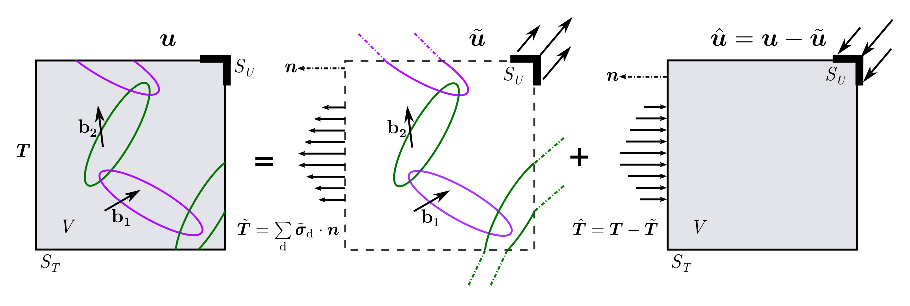
\includegraphics[width=\linewidth]{fem_ddd.eps}
	\caption[Coupling Discrete Dislocation Dynamics to Finite Element Methods.]{The \kwd{dl} ensemble in a volume $ V $ is bounded by surface $ S $. First, the traction field $ \sum_{\textrm{d}} \tns{\tilde{\sigma}}_{\textrm{d}} $ due to the \kwd{dl} ensemble is evaluated at the surface. Then, a traditional \kwd{fem} or \kwd{bem} calculates the image traction field $ \tns{\hat{\sigma}} \times \vec{n} $. Which is then fed back to the \kwd{ddd} problem to evolve the \kwd{dl} positions and repeat the cycle. Image edited from \cite{analytical_integration_of_the_forces_induced_by_dislocations_on_a_surface_element}.}
	\label{f:fem_ddd}
\end{figure}
\section{Extracting Surface Nodes}
The \kwd{fem} coupler arranges the nodes starting on the $ xz $-plane where $ y = 0, \ldots, n \mathrm{d}y,~n\in \mathbb{N} $. However in order to couple \kwd{ddd} to \kwd{fem} we only require the surface nodes where displacements are not calculated. Because we're working with rectangular prisms, we can easily pick out the surface nodes using a search algorithm with a logical mask. MATLAB and Fortran provide vector intrinsics that allow one to do so. \Cref{f:fem_surf_nodes} illustrates only the surface nodes according to our implementation's node arrangement---which is the $ xz $-plane going from $ y = y_{\textrm{min}} \to y = y_{\textrm{max}} $.
\begin{figure}
	\centering
	\begin{subfigure}[b]{0.45\linewidth}
		\centering
		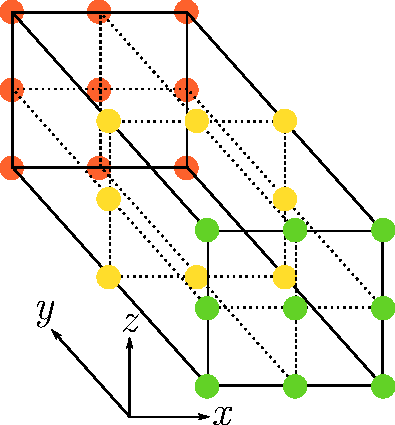
\includegraphics[width=\linewidth]{fem_surf_nodes.pdf}
		\caption[Surface nodes of our \kwd{fe} model.]{Arrangement of the surface nodes of our \kwd{fe} model. \kwd{fe} nodes are arranged in chunks of $ \Delta x \Delta z $ nodes in our implementation, but we only want the surface nodes.}
		\label{f:fem_surf_nodes}
	\end{subfigure}
	~
	\begin{subfigure}[b]{0.45\linewidth}
		\centering
		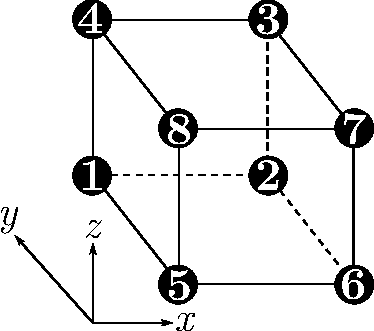
\includegraphics[width=\linewidth]{fe_numbering.pdf}
		\caption[Single finite element node numbering.]{Single \kwd{fe} node numbering. It is necessary to know which \kwd{fe} plane corresponds to which node labels. This lets us design the auxiliary matrix that selects nodes according to the planes we want to extract.}
		\label{f:fe_numbering}
	\end{subfigure}
	\caption[Finite Element node arrangement for coupling to Discrete Dislocation Dynamics.]{\kwd{fe} node arrangement for coupling to \kwd{ddd}.}
	\label{f:fem_node_arr}
\end{figure}
However, due to the nature of the analytical solutions in \cref{c:lin_rect}, we need all the surface nodes of the rectangular faces for which there are no displacements. This means that edge nodes are shared between 2 adjacent faces and corner nodes between 3 adjacent faces. In order to properly apply the logical mask to find \emph{only} the surface nodes need to know that each \kwdp{fe}' nodes are numbered according to \cref{f:fe_numbering}.

Using \cref{f:fem_node_arr} one can work out which nodes are of interest to whichever surface is being extracted. The ordering of the nodes in the final array will depend on the definition of the problems in \cref{c:lin_rect}.

Node selection remains an expensive operation and minimising array indexing is of the utmost importance for the best perfomance. Selecting nodes in the traditional sense, i.e. with code branching such as \texttt{if statements} or \texttt{case selection} is unmantainable, verbose and very prone to mistakes. The issue was solved by introducing an auxiliary matrix which defines various parameters that aid node selection and greatly reduces code size, improves readability, and eliminates the need for code branching. The matrix can be constructed utilising \cref{f:fem_node_arr} in order to know which nodes correspond to which \kwd{fe} planes. The $ p\textsuperscript{th} $ column of the matrix\footnote{MATLAB uses column-major ordering, so this gives us the best performance for vectorised code.} corresponds to the $ p\textsuperscript{th} $ plane (according to an arbitrary plane numbering) and is defined as,
\begin{align}\label{e:surf_node_util_vec}
	\vec{V_{p}}^{\mathsf{T}} =
	\begin{bmatrix}
		L_{1p} & L_{2p} & \cdots & L_{Np} & A_{p} & C_{p}
	\end{bmatrix}\,,
\end{align}
where $ L_{np} $ is the numeric label for node $ n $ as given by \cref{f:fem_node_arr}, $ A_{p} $ is the area of the plane, and $ C_{p} $ is the numeric label of the orthogonal coordinate to the plane $ C_{p} = 1, ~2, ~3 $ for the $ x, ~y, ~z $ coordinates respectively. $ A_{p} $ lets us segment our output and transitional arrays so that the only data being modified is that which corresponds to the correct plane and $ C_{p} $ lets us know which coordinate we must use in our selection criteria. Using our particular node labelling scheme (with dimensions $ \Delta x,~ \Delta y,~ \Delta z $ respectively in the $ x,~ y,~ z $ directions), the matrix is defined as,
\begin{align}\label{e:surf_node_util}
	\mtx{V} =
	\begin{bmatrix}
		5                 & 2                 & 6                 & 1                 & 5                 & 4                 \\
		1                 & 6                 & 5                 & 2                 & 6                 & 3                 \\
		8                 & 3                 & 7                 & 4                 & 1                 & 8                 \\
		4                 & 7                 & 8                 & 3                 & 2                 & 7                 \\
		\Delta y \Delta z & \Delta y \Delta z & \Delta x \Delta z & \Delta x \Delta z & \Delta x \Delta y & \Delta x \Delta y \\
		1                 & 1                 & 2                 & 2                 & 3                 & 3
	\end{bmatrix}\,.
\end{align}
The information codified in \cref{e:surf_node_util} lets us index and process only the necessary columns to extract the surface nodes we're interested in. The advantage of this setup over a naïve implementation is that it can be relatively easily expanded, maintained, and is general enough that it lends itself to a variety of selection criteria. The columns from left to right (1 to 6) represent:
\begin{inparaenum}[{face} 1 $ \equiv $]
	\item $ \min(x),~ yz $-plane;
	\item $ \max(x),~ yz $-plane;
	\item $ \min(y),~ xz $-plane;
	\item $ \max(y),~ xz $-plane;
	\item $ \min(z),~ xy $-plane;
	\item $ \max(z),~ xy $-plane.
\end{inparaenum}

It is important to make sure the nodes are extracted in a self consistent manner because the problem definitions in \cref{c:lin_rect} assume a specific node ordering. In particular, the labelling chirality must remain the same. This is due to the fact that the problems in \cref{c:lin_rect} utilise internal coordinates derived from a set of basis vectors, and scalar projections onto them. If the relationship between the vectors is kept, but the chirality is different (opposite) the calculated quantities will have the wrong sign. If however the relationship between the vectors is different to the problem formulation, the program will crash due to division by 0. Self-consistency was achieved by placing an imaginary observer inside the \kwd{fe} model facing the $ \min(x),~ yz $-plane (face 1) and rotating it to view all 6 planes according to \cref{f:surf_node_plane}.
\begin{figure}
	\centering
	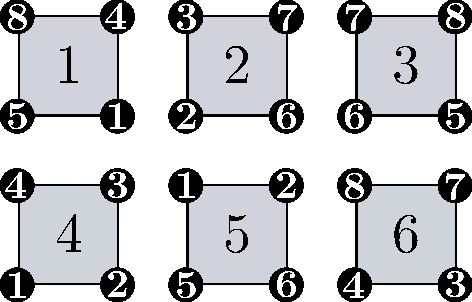
\includegraphics[width=0.75\linewidth]{surf_node_plane.pdf}
	\caption[Self-consistent, chirality preserving surface planes.]{Self-consistent, chirality preserving surface planes. Plane and node numbering according to the columns of \cref{e:surf_node_util} and \cref{f:fem_node_arr}.}
	\label{f:surf_node_plane}
\end{figure}
\section{Mapping Forces}
\begin{algorithm}
	\caption{If $ \vec{\hat{F}} $'s columns are arranged the same way as $ \vec{\gamma_{t}} $.}
	\begin{algorithmic}[1]
		\State\Comment{Loop through the array containing the node labels of the relevant surface nodes.}
		\For{$ i = 0;\, i < \rvar{length}(\vec{\gamma_{t}});\, i++$}
		\State\Comment{Save the global node label for the current iteration.}
		\State $ n \gets \vec{\gamma_{t}}[i] $
		\State\Comment{Use the node label to find a vector with the linearised index of all surface nodes whose labels correspond to the node whose forces we want to pass on to the \kwd{fem} coupler.}
		\State $ \vec{L} \gets \rvar{find}(\mtx{N_{L}} == n) $
		\State\Comment{Loop over coordinates.}
		\For{$ k = 0;\, k < 3;\, k++ $}
		\State\Comment{Use global node label vector to index the force array from the analytical force calculation due to dislocations on surface nodes. Multiplied by 3 because there are three coordinates per node. We sum the forces from the analytical calculation because the same global node can be part of multiple surface elements. We add $ k $ because the $ x,~y,~z $ coordinates are consecutively stored in $ \mtx{F_{n}} $.}
		\State $ \mtx{\hat{F}}[3\times \vec{L} + k] \gets \mtx{\hat{F}}[3\times \vec{L} + k] + \sum\mtx{F_{n}}[3\times \vec{L} + k]  $
		\EndFor
		\EndFor
	\end{algorithmic}
\end{algorithm}

%	\begin{algorithm}
%		\begin{algorithmic}[1]
%			content...
%		\end{algorithmic}
%	\end{algorithm}
\begin{figure}
	\centering
	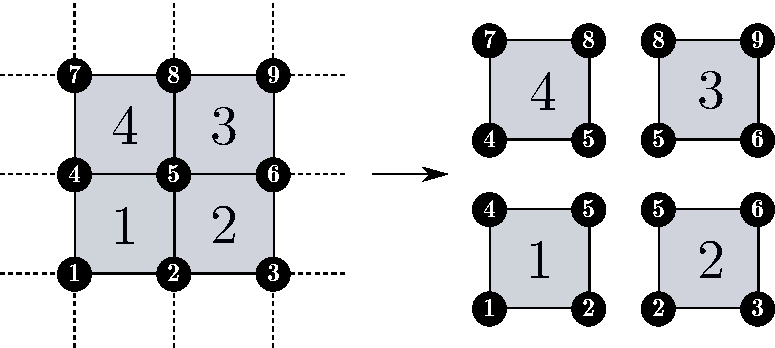
\includegraphics[width=\linewidth]{lrse_thread_map.pdf}
	\caption[Finite element nodes shared by multiple surface elements.]{\kwd{fe} nodes shared by multiple \kwdp{se}.}
	\label{f:fe_node_share}
\end{figure}

$ \vec{\hat{F}} $ only cares about the global node numbers, of which there are $ M $. The columns of $ \mtx{N_{L}},~ \mtx{F_{N}} $ represent the 4 nodes of a \kwd{se}, the rows represent the \kwd{se} they are part of. The column vector $ \vec{x} $ represents the $ x,~y,~z$-coordinates of the node-element or global node corresponding to their subscript. The column vector $ \vec{\gamma_{t}} $ is the list of global nodes for which the forces induced by dislocations must be calculated.
\begin{align}
	\vec{x_{e,n}}^{\mathsf{T}} & \equiv	\begin{bmatrix}
		x_{en} & y_{en} & z_{en}
	\end{bmatrix}, \quad
	\vec{\hat{x}_{n}}^{\mathsf{T}} \equiv	\begin{bmatrix}
		x_{n} & y_{n} & z_{n}
	\end{bmatrix}      \\
	\begin{split}
		\mtx{N_{L}} &=	\begin{bmatrix}
			l_{1,1} & l_{1,2} & l_{1,4} & l_{1,5} \\
			l_{2,2} & l_{2,3} & l_{2,5} & l_{2,6} \\
			l_{3,5} & l_{3,6} & l_{3,8} & l_{3,9} \\
			l_{4,4} & l_{4,5} & l_{4,7} & l_{4,8} \\
		\end{bmatrix}
	\end{split}
	, \quad
	\vec{\gamma} =   \begin{bmatrix}
		l_1    \\
		l_2    \\
		\vdots \\
		l_9
	\end{bmatrix}                          \\
	\begin{split}
		\mtx{F_{e}} &=	\begin{bmatrix}
			\vec{x_{1,1}} & \vec{x_{1,2}} & \vec{x_{1,3}} & \vec{x_{1,4}} \\
			\vec{x_{2,1}} & \vec{x_{2,2}} & \vec{x_{2,3}} & \vec{x_{2,4}} \\
			\vec{x_{3,1}} & \vec{x_{3,2}} & \vec{x_{3,3}} & \vec{x_{3,4}} \\
			\vec{x_{4,1}} & \vec{x_{4,2}} & \vec{x_{4,3}} & \vec{x_{4,4}} \\
		\end{bmatrix}
	\end{split}
	,\quad
	\vec{\hat{F}} = 	\begin{bmatrix}
		\vec{\hat{x}_{1}} \\
		\vec{\hat{x}_{2}} \\
		\vec{\hat{x}_{3}} \\
		\vec{\hat{x}_{4}}
	\end{bmatrix}\,.\label{e:force_imp}
\end{align}


\chapter{Analytical Forces Induced by Dislocations on Linear Rectangular Surface Elements}
\label{c:lin_rect}
%
\section{Forces Exerted by a Dislocation Line Segment on Linear Rectangular Surface Elements}
\label{s:f_lin_rect}
%
Coupling discrete dislocation dynamics to finite element method requires the traction field $ \tns{\sigma^{\infty}}(\vec{x}) \cdot \vec{n}(\vec{x}) $ to be distributed among the set of relevant discrete nodes of a finite element or boundary element model. This is usually achieved as follows,
\begin{align}\label{eq:ddd_fem_force}
	\vec{F}^{(m)} = \int_{S^{e}} \left[\tns{\sigma^{\infty}}(\vec{x}) \cdot \vec{n}(\vec{x})\right] N_{m}(\vec{x})\; \rvar{d}S_{e}\,,
\end{align}
where $ \rvar{d}S_{e} $ is the infinitesimal surface element with surface area $ S_{e} $. $ N_{m}(\vec{x}) $ are so-called shape functions (interpolation functions) that distribute  the traction field among the surface element's nodes.

The problematic singularity associated with the classical Volterra dislocation is avoided by using the non-singular formulation of \citet{a_non-singular_continuum_theory_of_dislocations}. The stress field of a dislocation in a homogenous infinite linear elastic domain can be calculated as a contour integral along the loop \cite{mura_t},
\begin{align}\label{eq:field_stress}
	\sigma_{ij}^{\infty}(\vec{x}) = C_{ijkl} \oint \epsilon_{lnh} C_{pqmn} \dfrac{\partial G_{kp}(\vec{x} - \vec{x'})}{\partial x_{q}} b_{m} \rvar{d}x'_{h}\,,
\end{align}
where $ C_{ijkl} $ is the elastic stiffness matrix, $ \epsilon_{lnh} $ the permutation operator, $\vec{b}$ the Burgers vector, $ \vec{x'} $ the coordinate that spans the dislocation, and $ G_{kp}(\vec{x} - \vec{x'}) $ is Green's function of elasticity \cite{mura_t}. $ G_{kp}(\vec{x} - \vec{x'}) $ is defined as the displacement component in the $ x_{k} $ direction at point $ \vec{x} $ due to a force applied in the $ x_{p} $ direction at point $ \vec{x'} $. The traditional singularity comes from taking the Burgers vector distribution as a delta function. \citet{a_non-singular_continuum_theory_of_dislocations} proposed an alternative definition of $ G_{kp}(\vec{x} - \vec{x'}) $ which has a wider isotropic spread mainly localised in a radius $ a $ around the dislocation core,
\begin{align}\label{eq:elastic_green_func}
	G_{ij}(\vec{x} - \vec{x'}) = \dfrac{1}{8\pi \mu}\left[ \delta_{ij} \partial_{pp} - \dfrac{1}{2(1-\nu)} \partial_{ij} \right] R_{a}\,,
\end{align}
where $ \mu $, $ \nu $ are the isotropic shear modulus and Poisson's ratio respectively, $ \delta_{ij} $ is the Kronecker Delta, $ \partial_{x_{1} \ldots\, x_{n}} \equiv \dfrac{\partial^{n}}{\partial x_{1} \ldots\, \partial x_{n}}$. $ R_{a} $ is the defined as,
\begin{subequations}
	\begin{align}\label{eq:ra}
		R_{a}(\vec{x}) & = R(\vec{x}) * w(\vec{x}) = \int R(\vec{x} - \vec{x'}) w(\vec{x'}) \rvar{d}^{3}\vec{x'}\nn
		               & = \sqrt{R^{2} + a^{2}}                                                                     \\
		w(\vec{x})     & = \dfrac{15 a^{4}}{8\pi (R^{2} + a^{2})^{7/2}}\,,
	\end{align}
\end{subequations}
where $ w(\vec{x}) $ is the isotropic Burgers vector distribution derived in the appendix of \cite{a_non-singular_continuum_theory_of_dislocations}, $ \vec{x} = (x, y, z) $ and $ R(\vec{x}) = \sqrt{x^{2} + y^{2} + z^{2}} $.

For two dislocation nodes (1, 2) connected by straight line segments \cref{eq:field_stress} becomes,
\begin{align}\label{eq:two_node_stress_field}
	\tns{\sigma}^{(12)}(\vec{x}) =
	\begin{split}
		&-\dfrac{\mu}{8\pi} \int\limits_{\vec{x_{1}}}^{\vec{x_{2}}} \left( \dfrac{2}{R_{a}^{3}} + \dfrac{3 a^{2}}{R_{a}^{5}} \right) \left[ \left( \vec{R} \times \vec{b} \right) \otimes \rvar{d}\vec{x'} + \rvar{d}\vec{x'} \otimes \left( \vec{R} \times \vec{b} \right) \right]\\
		%
		&+ \dfrac{\mu}{4\pi (1 - \nu)} \int\limits_{\vec{x_{1}}}^{\vec{x_{2}}} \left( \dfrac{1}{R_{a}^{3}} + \dfrac{3 a^{2}}{R_{a}^{5}} \right) \left[ \left(\vec{R} \times \vec{b}\right)\cdot \rvar{d}\vec{x'} \right] \mtx{I}_{2}\\
		%
		&- \dfrac{\mu}{4\pi (1 - \nu)} \int\limits_{\vec{x_{1}}}^{\vec{x_{2}}} \dfrac{1}{R_{a}^{3}} \left[ \left(\vec{b} \times \rvar{d}\vec{x'}\right) \otimes \vec{R} + \vec{R} \otimes \left(\vec{b} \times \rvar{d}\vec{x'}\right) \right]\\
		&+ \dfrac{\mu}{4\pi (1 - \nu)} \int\limits_{\vec{x_{1}}}^{\vec{x_{2}}} \dfrac{3}{R_{a}^{5}} \left[ \left( \vec{R} \times \vec{b} \right) \cdot \rvar{d}\vec{x'} \right]\vec{R} \otimes \vec{R}
	\end{split}\,.
\end{align}
\begin{figure}
	\centering
	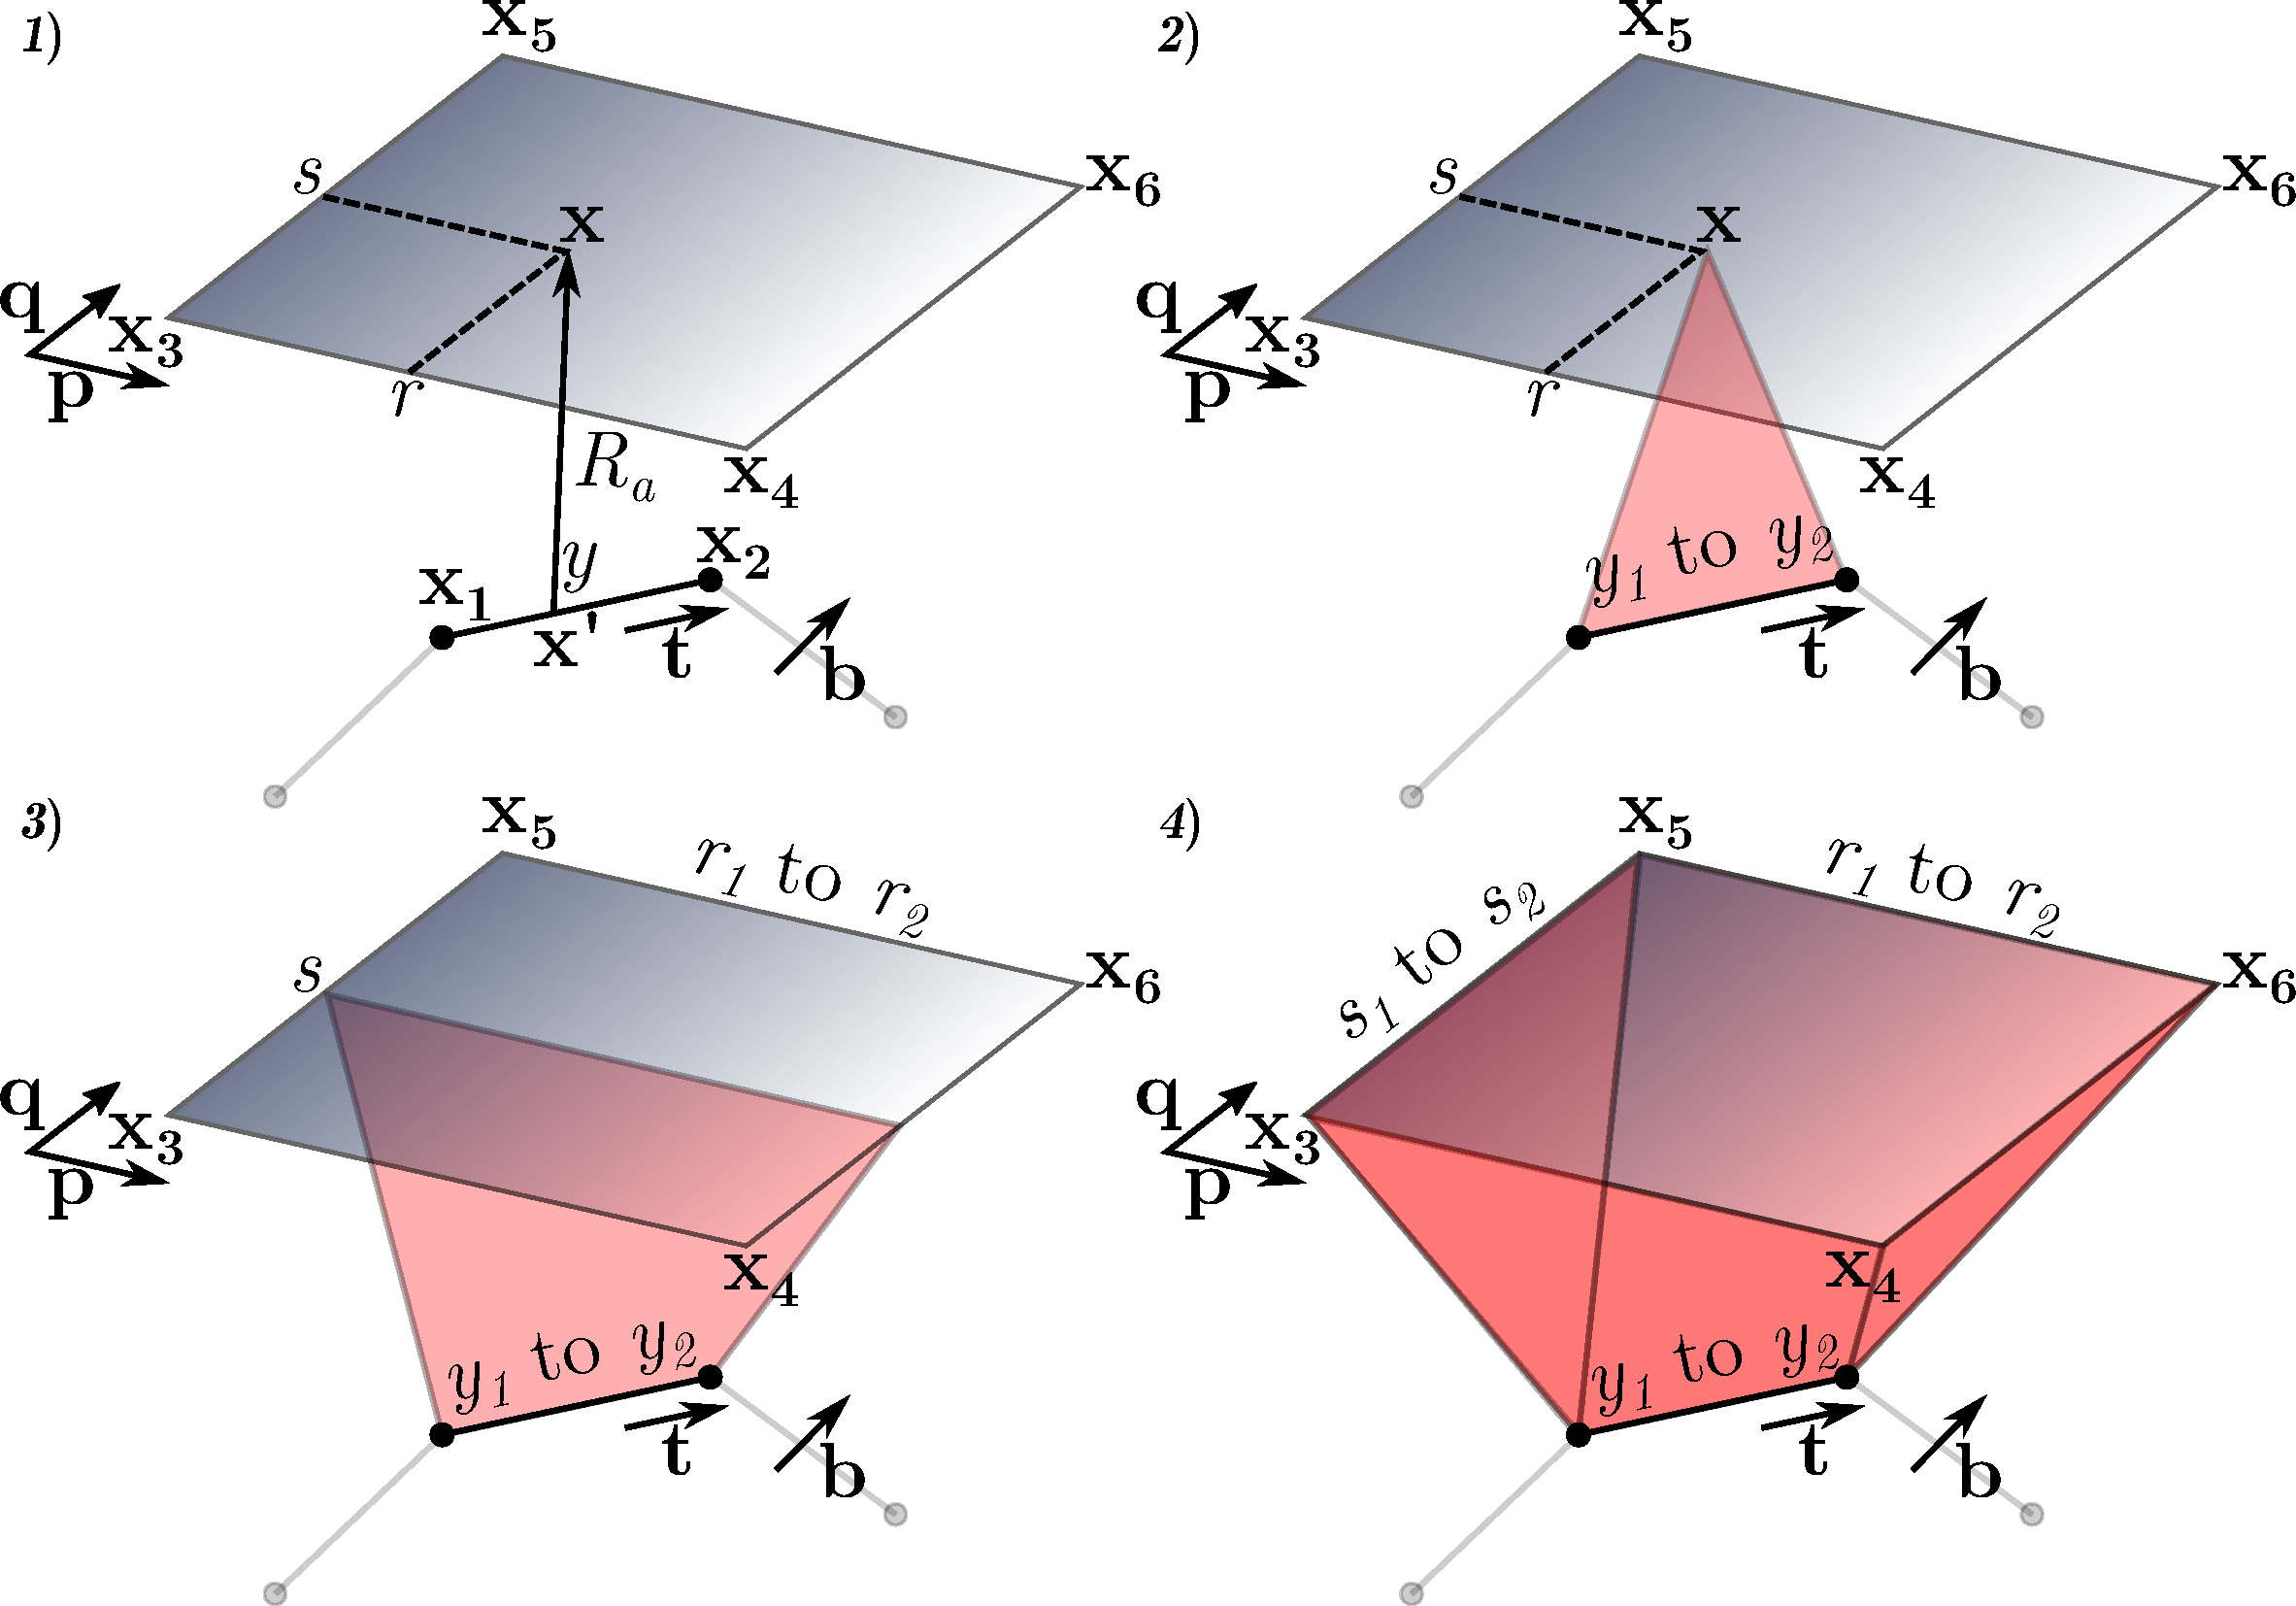
\includegraphics[width=\linewidth]{force_calc_linear_rectangle.pdf}
	\caption[Diagram of the analytical force calculation on linear rectangular surface elements.]{Diagram of the line integral method used to find analytical expressions for the forces exerted by dislocation lines on linear rectangular surface elements \cite{analytic_tractions}.
		\textit{1}) For any given point $ \vec{x} $ on the surface element and any given point $ \vec{x'}$ on the dislocation line segment, define distance $ R_{a} $.
		\textit{2}) Integrate from $ x_{1} \to x_{2} $ along line direction $ \vec{t} $.
		\textit{3}) Integrate from $ r_{1} \to r_{2} $ along vector $ \vec{p} $.
		\textit{4}) Integrate from $ s_{1} \to s_{2} $ along vector $ \vec{q} $.}
	\label{f:flrs}
\end{figure}
\subsection{Resolving Singularities when Dislocation Line Segments are Parallel to Surface Elements}
\label{ss:par_dln_se}
%
\begin{figure}
	\centering
	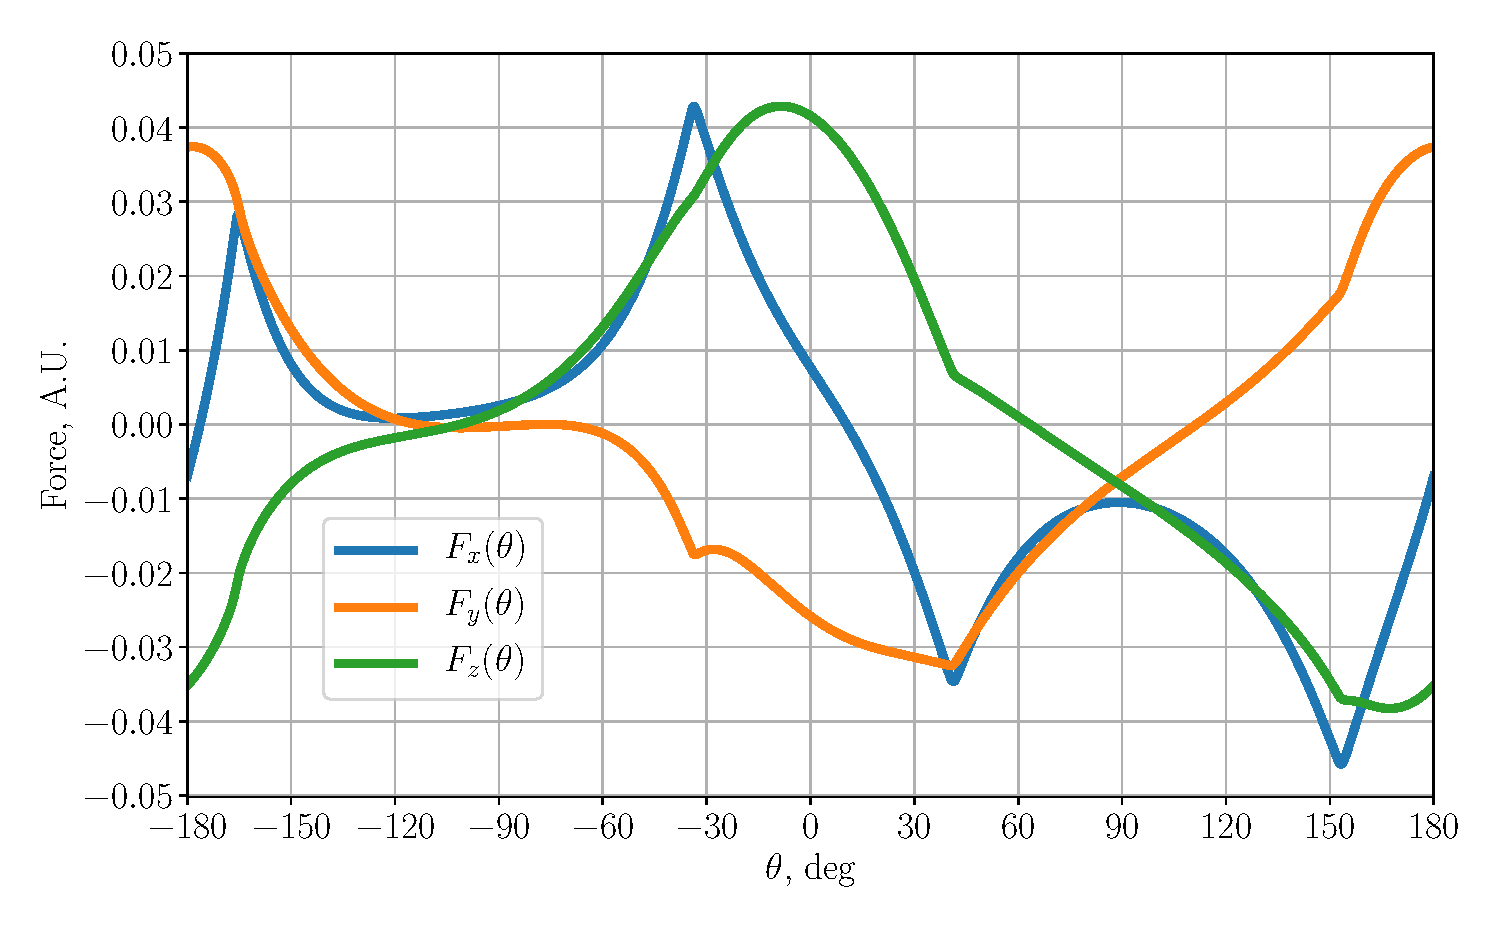
\includegraphics[width=\linewidth]{ftot_rotation_lin_rect.pdf}
	\caption[Avoiding singularities by rotating dislocation line segments.]{Effects of rotating a single dislocation line segment on the forces exerted by it on a linear rectangular surface element. The specific values of this function are not known \emph{a priori}, all that is known is that it must be periodic ($ T = 2\pi$) and have finite maximum and minimum values. The singularity is avoided by perturbing the angle $ \theta = 0 \to \theta = \pm \epsilon\,, \epsilon \gtrsim 0 $.}
	\label{f:rflrs}
\end{figure}
%
\savearabiccounter
% TODO #6
\chapter{Analytical Forces Induced by Dislocations on Quadratic Triangular Surface Elements}
\label{c:quad_triang}
	\section{Forces Exerted by a Dislocation Line Segment on Quadratic Triangular Surface Elements}
	\label{s:f_quad_triang}
	\begin{figure}
		\centering
		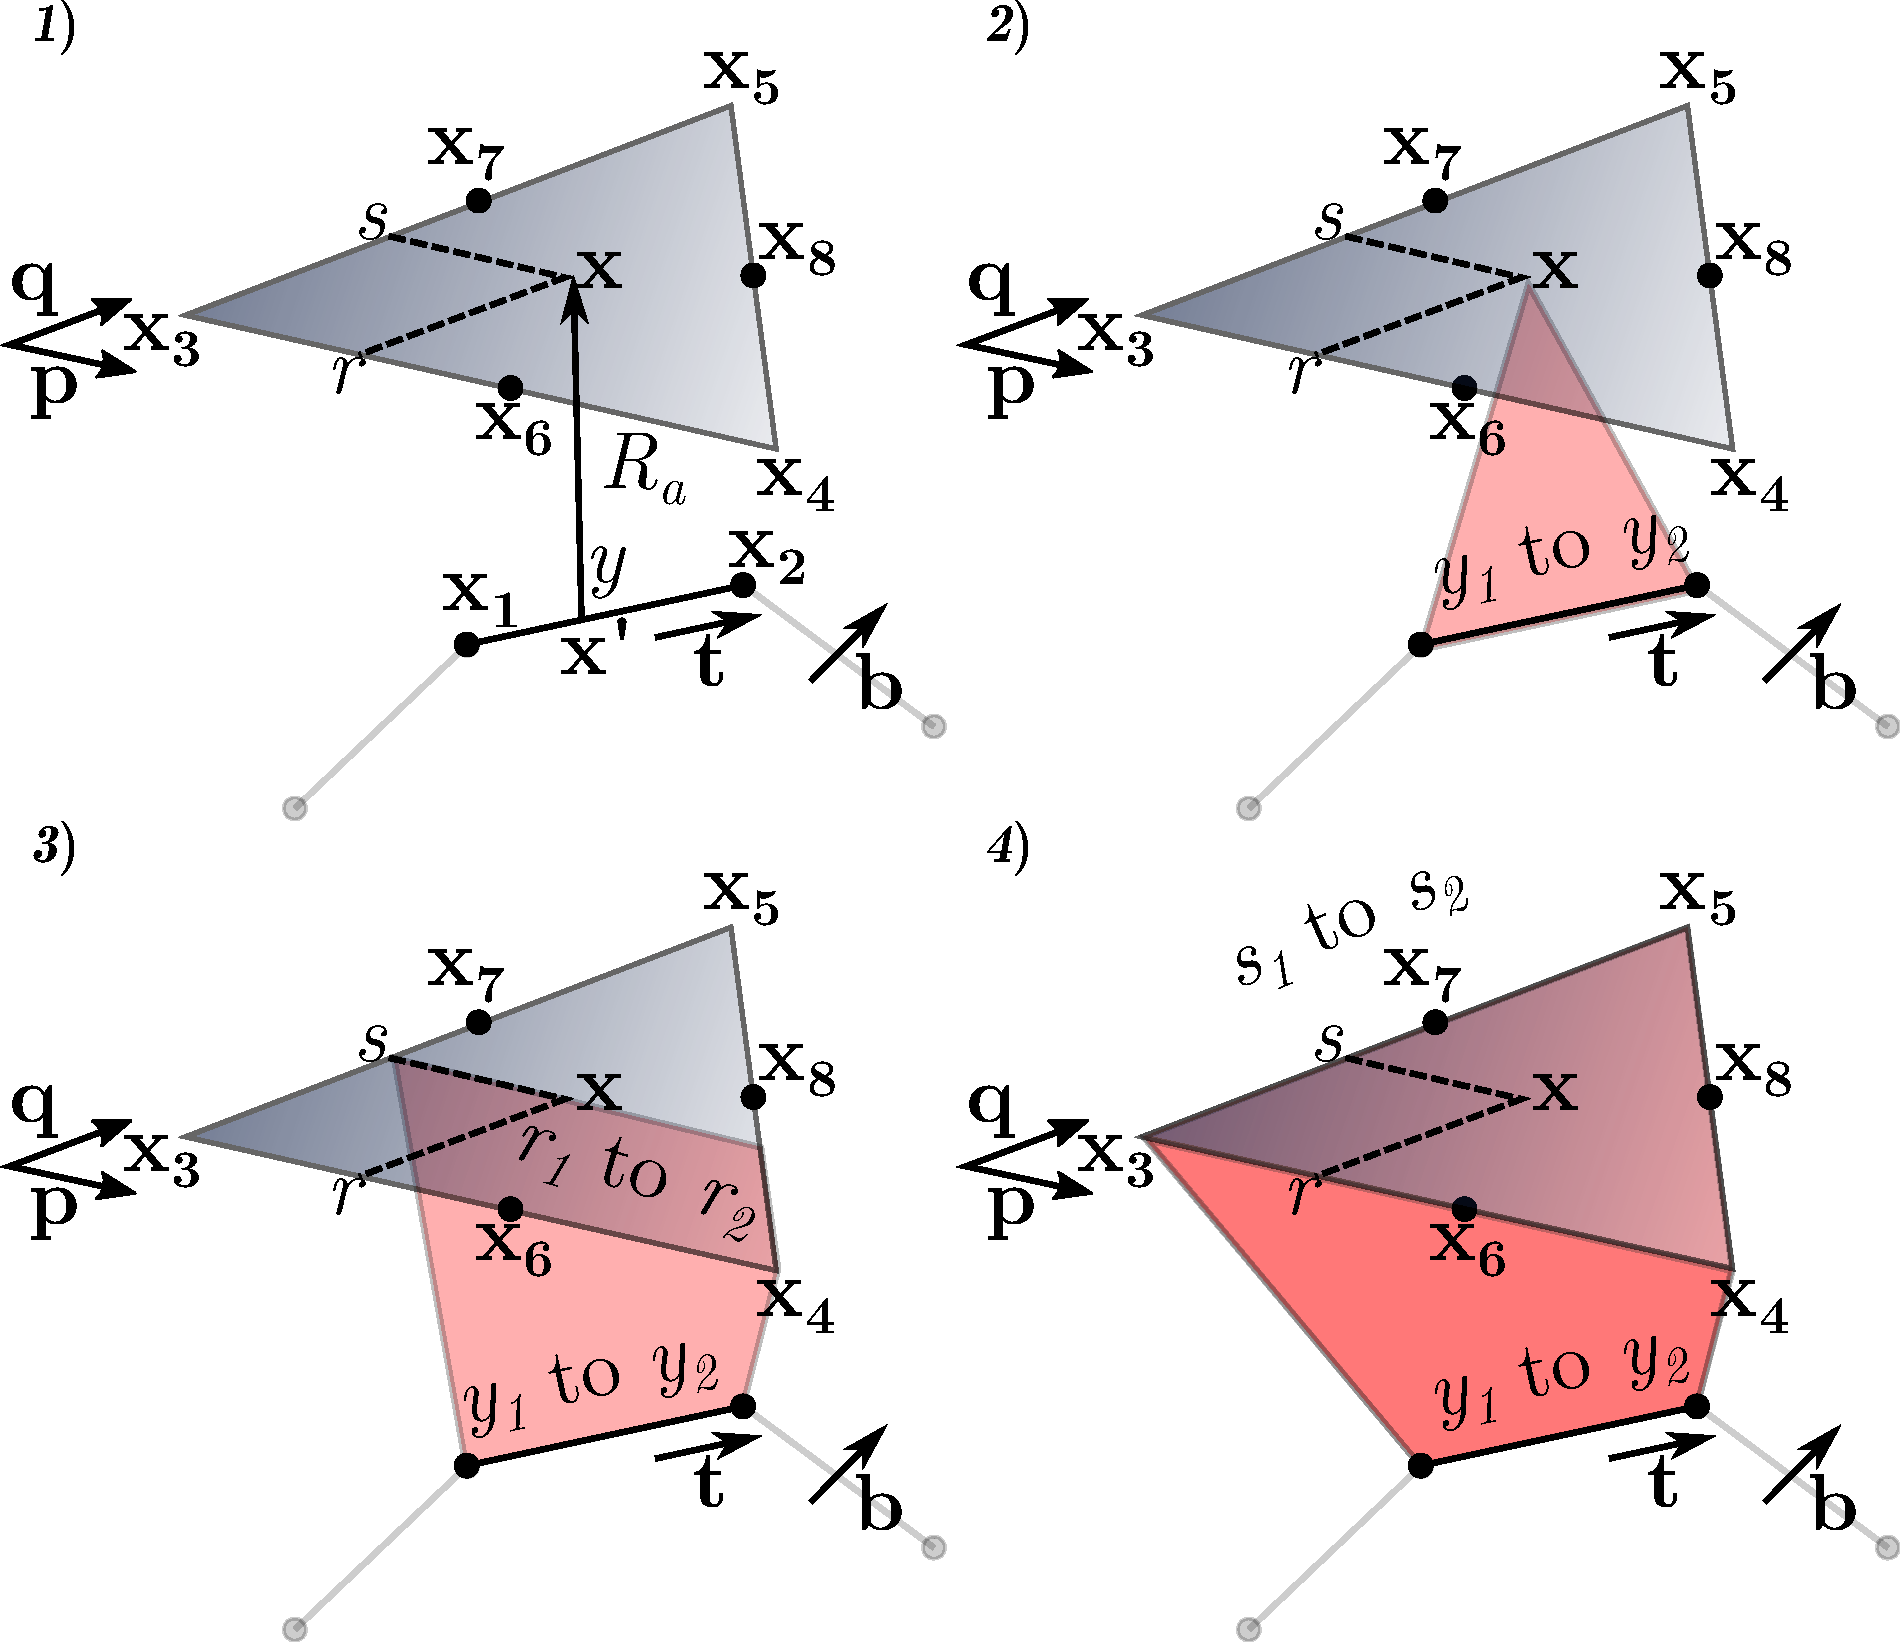
\includegraphics[width=\linewidth]{force_calc_quad_triangle.pdf}
		\caption[Diagram of the analytical force calculation on quadratic triangular surface elements.]{Diagram of the line integral method used to find analytical expressions for the forces exerted by \kwdp{dl} on quadratic triangular \kwdp{se}.}
		\label{f:fqts}
	\end{figure}
\savearabiccounter
\chapter{Parallelisation of the Analytical Forces Induced by Dislocations on Surface Elements}
\label{c:para_f_dln_se}
	%
	\section{Parallelisation on Graphics Processing Units}
	Efficient parallelisation requires \kwd{cma}, which means we have to be extremely careful when mapping CPU memory to device memory. The fact that threads work ``simultaneously''\footnote{Not quite but essentially simultaneously.} means that in order to obtain good performance, data which is to be ``simultaneously'' loaded into each thread must be contiguous. This maximises cache memory use and therefore reduces slow memory fetch operations to global or shared memory.
	
	The parallelisation was done only over the \kwdp{se} in order to avoid the undesirable and inefficient GPU branching that would occur under other schemes.
	
	The most natural form of parallelisation is to have blocks of $ 4n $ threads where $ n \leq 8 \in \mathbb{N}$. This also fits nicely into the 32 thread per warp paradigm.
	%
	\subsection{Data Mapping}
		%
		\begin{figure}
			\centering
			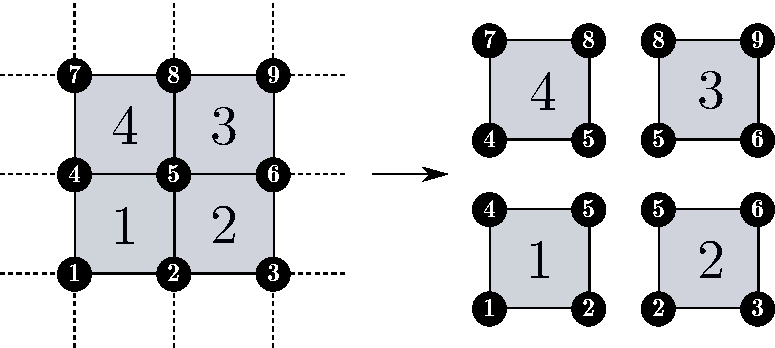
\includegraphics[width=\linewidth]{lrse_thread_map.pdf}
			\caption[Linear rectangular surface element mapping.]{Each linear rectangular \kwd{se} is mapped to one thread.}
			\label{f:lrse_map}
		\end{figure}
		%
		\subsubsection{Elements: Host $ \mapsto $ Device}
			%
			\begin{algorithm}
				\caption{Elements in host $ \mapsto $ device.}
				\label{a:ehd}
				\begin{algorithmic}[1]
					\Function{element\_host\_device\_map}{\hvar{\vec{X}[N][3\times E]}}
						\State{\Comment{Input, temporary, and output indices set to zero.}}
						\State{$ i,\, j,\, k \gets 0 $}
						\State{\Comment{\dvar{\vec{X}} accomodates all 3 coordinates of all $ N $ nodes in all $ E $ elements.}}
						\State{$ \dvar{\vec{X}} \gets $ malloc($ 3\times E\times N $)}
						\For{$(n = 0;\, n < N;\, n++)$} \Comment{Loop over nodes in element.}
							\State{\Comment{Set output index to point at the $ n\textsuperscript{th} $ node of the first coordinate of the first element.}}
							\State{$ k \gets j $}
							\For{$ (c = 0;\, c < 3;\, c++) $} \Comment{Loop over coordinates.}
								\State{\Comment{Set input index to point at the $ c\textsuperscript{th} $ coordinate of the first element of the $ n\textsuperscript{th} $ node.}}
								\State{$ i \gets c $}
								\For{$ (e = 0;\, e < E;\, e++) $} \Comment{Loop over elements.}
									\State{$ \dvar{\vec{X}[k + e]} \gets \hvar{\vec{X}[n][i]} $}
									\State{\Comment{Advance output index to point at the $ n\textsuperscript{th} $ node of the $ c\textsuperscript{th} $ coordinate of the first element.}}
									\State{$ i \gets i + 3 $}
								\EndFor
								\State{\Comment{Advance output index to point at the $ n\textsuperscript{th} $ node of the $ c\textsuperscript{th} $ coordinate of the first element.}}
								\State{$ k \gets k + E \times N $}
							\EndFor
							\State{\Comment{Advance temporary index to point at the $ (n+1)\textsuperscript{th} $ node of the first coordinate of the first element.}}
							\State{$ j \gets j + E $}
						\EndFor
						\State{\Return{\dvar{\vec{X}}}}
					\EndFunction
				\end{algorithmic}
			\end{algorithm}
		\subsubsection{Elements: Device $ \mapsto $ Thread}
			\begin{algorithm}
				\caption{Elements in device $ \mapsto $ thread.}
				\label{a:edt}
				\begin{algorithmic}[1]
						\GPUFunction[element\_device\_thread\_map]{\dvar{\vec{X}[3\times E\times N]}, \tvar{\vec{X}[N][3]}}
						\State{\Comment{Thread, input indices.}}
						\State{$ \rvar{idx},\, i \gets \rvar{threadIdx}.x + \rvar{blockIdx}.x\times \rvar{blockDim}.x $}
						\For{$ (c = 0;\, c < 3;\, c++) $}\Comment{Loop over elements.}
							\For{$ (n = 0;\, n < N;\, n++) $}\Comment{Loop over nodes in element.}
								\State{$ \tvar{\vec{X}[n][c]} \gets \dvar{\vec{X}[i + n\times E]}$}
							\EndFor
							\State{$ i \gets i + E\times N $}
							\Comment{Advance input index to the $(n+1)\textsuperscript{th}$ node of element $i$.}
						\EndFor
						\State{\Return{\tvar{\vec{X}[n][c]}}}
					\EndGPUFunction
				\end{algorithmic}    	
			\end{algorithm}
		\subsubsection{Force: Thread $ \xmapsto{+} $ Device}
			\begin{algorithm}
				\caption{Force in thread $ \xmapsto{+} $ device.}
				\begin{algorithmic}[1]
						\GPUFunction[add\_force\_thread\_device]{\tvar{\vec{F_{n}}[N][3]}, \tvar{\vec{F_{e}}[3]}, \dvar{\vec{F_{n}}[3\times E\times N]},\newline{}\dvar{\vec{F_{e}}[3\times E]}, \rvar{idx}}
						\State{\Comment{Nodal force.}}
						\State{\Comment{Set output index to whatever parallelisation index is given to the function. In this case the same index we use for the main parallelisation.}}
						\State{$ i \gets \rvar{idx} $}
						\For{$ (n = 0;\, n < N;\, n++) $} \Comment{Loop over nodes.}
							\For{$ (c = 0;\, c < 3;\, c++) $} \Comment{Loop over coordinates.}
								\State{\Comment{Ensure nodal forces are correctly added and mapped from local thread memory to global device memory.}}
								\State{atomicAdd(\dvar{\vec{F_{n}}[i + c\times E\times N]}, \tvar{\vec{F_{n}}[n][c]})}
							\EndFor
							\State{\Comment{Displace output index to point at the first coordinate of the $ (n+1)\textsuperscript{th} $ node of the \rvar{idx}\textsuperscript{th} \kwd{se}.}}
							\State{$ i \gets i + E $}
						\EndFor
						\State{\Comment{Total force.}}	
						\State{$ i \gets \rvar{idx} $} \Comment{Reset output index.}
						\For{$ (c = 0;\, c < 3;\, c++) $} \Comment{Loop over coordinates.}
							\State{atomicAdd(\dvar{\vec{F_{e}}[i]}, \tvar{\vec{F_{e}}[c]})}
							\State{\Comment{Advance the output index to point at the $ (i+1)\textsuperscript{th} $ coordinate of the $ \rvar{idx}\textsuperscript{th} $ \kwd{se}.}}
							\State{$ i \gets i + E $}
						\EndFor
						\State{\Return{\dvar{\vec{F_{n}}}, \dvar{\vec{F_{e}}}}}
					\EndGPUFunction
				\end{algorithmic}
			\end{algorithm}
		\subsubsection{Force (Parallelise over Dislocations): Thread $ \xmapsto{+} $ Device}
			\begin{algorithm}
				\caption{Force (parallelise over dislocations) in thread $ \xmapsto{+} $ device.}
				\begin{algorithmic}[1]
					\GPUFunction[dln\_add\_force\_thread\_device]{\tvar{\vec{F_{n}}[N][3]}, \tvar{\vec{F_{e}}[3]},\newline{}\dvar{\vec{F_{n}}[3\times E\times N]}, \dvar{\vec{F_{e}}[3\times E]}, $ k $}
						\State{\Comment{Nodal force.}}
						\State{\Comment{Set output index to correspond to whatever \kwd{se} we're on. By parallelising over dislocation lines, we must loop through \kwdp{se} in the main code, this is the value of $ k $ we provide. Multiply by 3 and $ N $ because each \kwd{se} has 3 coordinates and $ N $ nodes.}}
						\State{$ i \gets 3\times N\times k $}
						\State{$ j \gets 0 $} \Comment{Auxiliary index.}
						\For{$ (n = 0;\, n < N;\, n++) $} \Comment{Loop over nodes.}
							\For{$ (c = 0;\, c < 3;\, c++) $} \Comment{Loop over coordinates.}
								\State{\Comment{Ensure nodal forces are correctly added and mapped from local thread memory to global device memory.}}
								\State{atomicAdd(\dvar{\vec{F_{n}}[i + j + c]}, \tvar{\vec{F_{n}}[n][c]})}
							\EndFor
							\State{\Comment{Displace auxiliary index to point at the first coordinate of the $ (n+1)\textsuperscript{th} $ node of the $ k \textsuperscript{th}$ \kwd{se}.}}
							\State{$ j \gets j + 3 $}
						\EndFor
						\State{\Comment{Total force.}}
						\State{\Comment{Set auxiliary index to point at the first coordinate of the $ k\textsuperscript{th} $ \kwd{se}.}}
						\State{$ j \gets 3\times k $}
						\For{$ (c = 0;\, c < 3;\, c++) $} \Comment{Loop over coordinates.}
							\State{atomicAdd(\dvar{\vec{F_{e}}[j+c]}, \tvar{\vec{F_{e}}[c]})}
						\EndFor
						\State{\Return{\dvar{\vec{F_{n}}}, \dvar{\vec{F_{e}}}}}
					\EndGPUFunction
				\end{algorithmic}
			\end{algorithm}
		\subsubsection{Nodal Force: Device $ \mapsto $ Host}
			\begin{algorithm}
				\caption{Nodal force in device $ \mapsto $ host.}
				\begin{algorithmic}[1]
					\Function{fx\_device\_host\_map}{\dvar{\vec{F_{n}}[3\times E\times N]}, \hvar{\vec{F_{n}}[N][3\times E]}}
						\State{$ i,~j \gets 0 $} \Comment{Set input and output indices to zero.}
						\For{$ n = 0;\, n < N;\, n++ $} \Comment{Loop over nodes.}
							\State{$ j \gets 0 $} \Comment{Reset output index to point at the first element.}
							\For{$ e = 0;\, e < E;\, e++ $} \Comment{Loop over elements.}
								\For{$ c = 0;\, c < 3;\, c++ $} \Comment{Loop over coordinates.}
									\State{$ \hvar{\vec{F_{n}}[n][j + c]} = \dvar{\vec{F_{n}}[i + e + c\times E\times N]} $}
								\EndFor
								\State{\Comment{Advance output index to point at the first coordinate of the $ (e+1)\textsuperscript{th} $ element.}}
								\State{$ j \gets j + 3 $}
							\EndFor
							\State{\Comment{Advance input index to point at the first coordinate of the $ (n+1)\textsuperscript{th} $ node of the first element.}}
							\State{$ i \gets i + E $}
						\EndFor
						\State{\Return{\hvar{\vec{F_{n}}}}}
					\EndFunction
				\end{algorithmic}
			\end{algorithm}
		\subsubsection{Total Force: Device $ \mapsto $ Host}
			\begin{algorithm}
				\caption{Total force in device $ \mapsto $ host.}
				\begin{algorithmic}[1]
					\Function{ftot\_device\_host\_map}{\dvar{\vec{F_{e}}[3\times E]}, \hvar{\vec{F_{e}}[3\times E]}}
						\State{$ i \gets 0 $} \Comment{Set output index to zero.}
						\For{$ e = 0;\, e < E;\, e++ $} \Comment{Loop over elements.}
							\For{$ c = 0;\, c < 3;\, c++ $} \Comment{Loop over coordinates.}
								\State{$ \hvar{\vec{F_{e}}[i + c]} = \dvar{\vec{F_{e}}[e + c\times E]} $}
							\EndFor
							\State{\Comment{Advance the output index to point at the first coordinate of the $ (e+1)\textsuperscript{th} $ surface element.}}
							\State{$ i \gets i + 3 $}
						\EndFor
						\State{\Return{\hvar{\vec{F_{e}}}}}
					\EndFunction
				\end{algorithmic}
			\end{algorithm}
	\begin{subequations}\label{e:fcne}
		\begin{align}
			\vec{X}_{en}			&\coloneqq	\left[x_{en},\, y_{en},\, z_{en}\right]\\
			\vec{X}_{(1\to E)n}		&\mapsto 	\vec{X}_{n} \nn
			\vec{X}_{n}				&\coloneqq	\left[x_{1n},\, y_{1n},\, z_{1n},\ldots,x_{En},\, y_{En},\, z_{En}\right]\label{se:xn_arr}\\
			\vec{X}_{1\to N}		&\mapsto	\vec{X}^{\textrm{SE}}\nn
			\vec{X}^{\textrm{SE}}	&\coloneqq 
			\begin{aligned}
				&\left[x_{11},\, \ldots,\, x_{E1},\, x_{12},\, \ldots,\, x_{E2},\, \ldots,\, x_{1N},\, \ldots,\, x_{EN}, \right.\\
				&\left.\,y_{11},\, \ldots,\, y_{E1},\, y_{12},\, \ldots,\, y_{E2},\, \ldots,\, y_{1N},\, \ldots,\, y_{EN}, \right.\\
				&\left.\,z_{11},\, \ldots,\, z_{E1},\, z_{12},\, \ldots,\, z_{E2},\, \ldots,\, z_{1N},\, \ldots,\, z_{EN}  \right]
			\end{aligned}
		\end{align}
	\end{subequations}
	where $ e $ is the \kwd{se} label, $ n $ the node label, $ E $ the number of \kwdp{se} in the scope. $ N $ the number of nodes in a \kwd{se}.
	
	Data-mapping according to \cref{a:fcne} and relabelling the nodes so they go from $ 0 \to N-1 $, the data from \cref{f:lrse_map} would be arranged in \kwd{devmem} like \cref{e:fcne_eg},
	\begin{align}\label{e:fcne_eg}
		\vec{X}^{\textrm{SE}} &= \begin{aligned}
			\left[\underbrace{h_{x},\, i_{x},\, f_{x},\, g_{x}}_{\mathbf{x_{0}}},\, 
			\underbrace{a_{x},\, b_{x},\, i_{x},\, h_{x}}_{\mathbf{x_{1}}},\, 
			\right.&\underbrace{i_{x},\, d_{x},\, e_{x},\, f_{x}}_{\mathbf{x_{2}}},\, 
			\underbrace{b_{x},\, c_{x},\, d_{x},\, i_{x}}_{\mathbf{x_{3}}},\\
			\ldots~y&\textrm{-coord}~\ldots,\\
			\ldots~z&\textrm{-coord}~\ldots]
		\end{aligned}
	\end{align}
	%
	
	In the GPU, each thread will cater to one \kwd{se} at a time. This means that each thread will have to extract the relevant data from the 1D array with length $ 3\times E\times N $ into four 1D arrays of length $ 3 $. The purpose of CNE mapping is to provide the \kwd{wrp} with \kwd{cma}. This is achieved via \cref{a:bcne}.
	
	
	Since \cref{a:bcne} is performed in a CUDA GPU, threads in a single block execute sequentially from,
	\begin{align}
		\rvar{threadIdx}.x &= 0 \to \rvar{threadIdx}.x = \rvar{blockDim}.x - 1\,,
	\end{align}
	while threads in different blocks execute in parallel. \Kwd{cma} is ensured by having each block load a cache line whose entries are contiguously accessed by the threads in the block. Using the same notation as \cref{a:fcne}, full cache line utilisation (optimal cache use) is achieved if cache lines can accomodate $ l $ entries given by \cref{e:opt_cache_len_bcne},
	\begin{align}
		\label{e:opt_cache_len_bcne}
		l =
		\begin{cases}
			a \times N \times E &,\, a > 0 \in \mathbb{N}\\
			&\textrm{or}\\
			\dfrac{1}{2^{a}} \times N \times E &,\, a \geq 0 \in \mathbb{N},\, N \times E \equiv 0\; (\bmod\; 2^{a})\,.
		\end{cases}
	\end{align}
	\Cref{f:fcne_eg} shows an example of \cref{a:bcne} up to the $ y $-coordinate.
	\begin{figure}
		\centering
		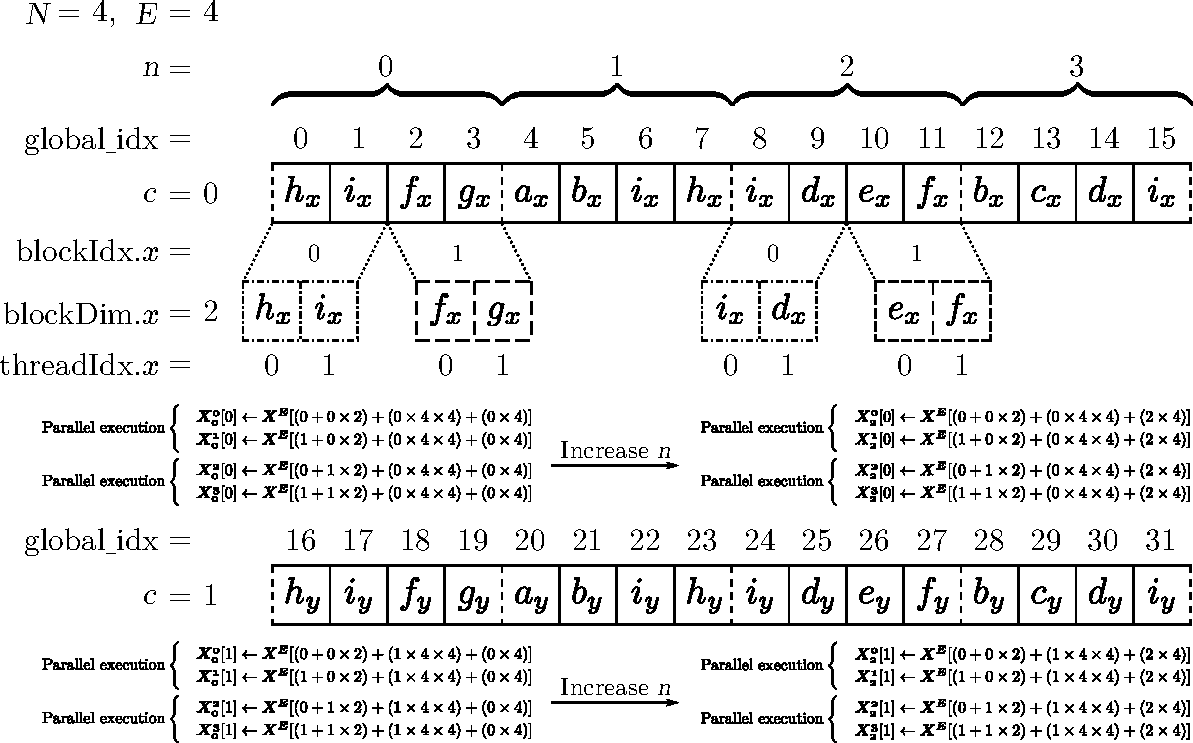
\includegraphics[width=\linewidth]{node_bmap.pdf}
		\caption[Example of the backward coodinate-node-element-map.]{Minimum working complete example of the backward coodinate-node-element-map. The explicit calculations of global indices correspond to subsituting the values for ``idx'' and ``idxi'' as in \cref{a:bcne}. $\vec{X_{a}^{b}}$ denotes a 1D array of length three containing the $ xyz $-coordinates of node $ a $ of element $ b $. Each thread concerns itself with only one element at a time. The dash-dot and dashed boxes represent cache lines for a thread block, the dotted line represents a memory fetch, and the dashed lines in $ \vec{X^{E}} $ represent steps of $ E $ entries (the start of the data for the next node of the element type we're dealing with). The memory operations are not shown twice to minimuse redundancy.}
		\label{f:fcne_eg}
	\end{figure}
	% Start: Code for generating figure e:opt_cache_len_bcne
	%\begin{align}%\label{f:fcne_eg}
	%	\vec{X}^{\textrm{SE}} &= 
	%							\begin{aligned}
	%								\left[\overbrace{h_{x},\, i_{x},\, f_{x},\, g_{x}}^{\mathbf{x_{3}}},\, 
	%								\overbrace{a_{x},\, b_{x},\, i_{x},\, h_{x}}^{\mathbf{x_{4}}},\, 
	%								\right.&\overbrace{i_{x},\, d_{x},\, e_{x},\, f_{x}}^{\mathbf{x_{5}}},\, 
	%								\overbrace{b_{x},\, c_{x},\, d_{x},\, i_{x}}^{\mathbf{x_{6}}},\\
	%								\overbrace{h_{y},\, i_{y},\, f_{y},\, g_{y}}^{\mathbf{x_{3}}},\, 
	%								\overbrace{a_{y},\, b_{y},\, i_{y},\, h_{y}}^{\mathbf{x_{4}}},\, 
	%								&\overbrace{i_{y},\, d_{y},\, e_{y},\, f_{y}}^{\mathbf{x_{5}}},\, 
	%								\overbrace{b_{y},\, c_{y},\, d_{y},\, i_{y}}^{\mathbf{x_{6}}},\\
	%								\overbrace{h_{z},\, i_{z},\, f_{z},\, g_{z}}^{\mathbf{x_{3}}},\, 
	%								\overbrace{a_{z},\, b_{z},\, i_{z},\, h_{z}}^{\mathbf{x_{4}}},\, 
	%								&\left.\overbrace{i_{z},\, d_{z},\, e_{z},\, f_{z}}^{\mathbf{x_{5}}},\, 
	%								\overbrace{b_{z},\, c_{z},\, d_{z},\, i_{z}}^{\mathbf{x_{6}}}\right]
	%\end{align}
	%\begin{align}
	%	\textrm{Parallel execution}
	%		&\begin{cases}
	%			&\vectorsym{X_{0}^{0}}[0] \gets \vectorsym{X^{E}}[(0+0\times 2) + (0\times 4 \times 4) + (0\times 4)]\nonumber\\
	%			&\vectorsym{X_{0}^{1}}[0] \gets \vectorsym{X^{E}}[(1+0\times 2) + (0\times 4 \times 4) + (0\times 4)]\nonumber\\
	%		\end{cases}\nonumber\\
	%	\textrm{Parallel execution}
	%		&\begin{cases}
	%			&\vectorsym{X_{0}^{2}}[0] \gets \vectorsym{X^{E}}[(0+1\times 2) + (0\times 4 \times 4) + (0\times 4)]\nonumber\\
	%			&\vectorsym{X_{0}^{3}}[0] \gets \vectorsym{X^{E}}[(1+1\times 2) + (0\times 4 \times 4) + (0\times 4)]\nonumber\\
	%		\end{cases}\nonumber\\
	%	\textrm{Parallel execution}
	%		&\begin{cases}
	%			&\vectorsym{X_{2}^{0}}[0] \gets \vectorsym{X^{E}}[(0+0\times 2) + (0\times 4 \times 4) + (2\times 4)]\nonumber\\
	%			&\vectorsym{X_{2}^{1}}[0] \gets \vectorsym{X^{E}}[(1+0\times 2) + (0\times 4 \times 4) + (2\times 4)]\nonumber\\
	%		\end{cases}\nonumber\\
	%	\textrm{Parallel execution}
	%		&\begin{cases}
	%			&\vectorsym{X_{2}^{2}}[0] \gets \vectorsym{X^{E}}[(0+1\times 2) + (0\times 4 \times 4) + (2\times 4)]\nonumber\\
	%			&\vectorsym{X_{2}^{3}}[0] \gets \vectorsym{X^{E}}[(1+1\times 2) + (0\times 4 \times 4) + (2\times 4)]\nonumber\\
	%		\end{cases}\nonumber\\
	%	%					
	%	\textrm{Parallel execution}
	%		&\begin{cases}
	%			&\vectorsym{X_{0}^{0}}[1] \gets \vectorsym{X^{E}}[(0+0\times 2) + (1\times 4 \times 4) + (0\times 4)]\nonumber\\
	%			&\vectorsym{X_{0}^{1}}[1] \gets \vectorsym{X^{E}}[(1+0\times 2) + (1\times 4 \times 4) + (0\times 4)]\nonumber\\
	%		\end{cases}\nonumber\\
	%	\textrm{Parallel execution}
	%		&\begin{cases}
	%			&\vectorsym{X_{0}^{2}}[1] \gets \vectorsym{X^{E}}[(0+1\times 2) + (1\times 4 \times 4) + (0\times 4)]\nonumber\\
	%			&\vectorsym{X_{0}^{3}}[1] \gets \vectorsym{X^{E}}[(1+1\times 2) + (1\times 4 \times 4) + (0\times 4)]\nonumber\\
	%		\end{cases}\nonumber\\
	%	\textrm{Parallel execution}
	%		&\begin{cases}
	%			&\vectorsym{X_{2}^{0}}[1] \gets \vectorsym{X^{E}}[(0+0\times 2) + (1\times 4 \times 4) + (2\times 4)]\nonumber\\
	%			&\vectorsym{X_{2}^{1}}[1] \gets \vectorsym{X^{E}}[(1+0\times 2) + (1\times 4 \times 4) + (2\times 4)]\nonumber\\
	%		\end{cases}\nonumber\\
	%	\textrm{Parallel execution}
	%		&\begin{cases}
	%			&\vectorsym{X_{2}^{2}}[1] \gets \vectorsym{X^{E}}[(0+1\times 2) + (1\times 4 \times 4) + (2\times 4)]\nonumber\\
	%			&\vectorsym{X_{2}^{3}}[1] \gets \vectorsym{X^{E}}[(1+1\times 2) + (1\times 4 \times 4) + (2\times 4)]\nonumber\\
	%		\end{cases}\nonumber
	%\end{align}
	% End: Code for generating figure e:opt_cache_len_bcne
	\subsubsection{Node Coordinate Element Map}
	%
	The node-coordinate-element (NCE) data mapping in \cref{e:fnce} is carried out by \cref{a:fnce}, each thread looks after a given \kwd{se}.
	\begin{algorithm}
		\caption{NCE data mapping.}
		\label{a:fnce}
		\begin{algorithmic}
			\ForAll{n nodes $ \in $ surface element}
			\ForAll{c coordinates $ \in [x,\, y,\, z] $}
			\ForAll{e surface elements $ \in $ surface mesh section}
			\State list.append(data of the $ n\textsuperscript{th}$ node with $ c\textsuperscript{th} $ coordinate of the $ e\textsuperscript{th} $ SE)
			\EndFor
			\EndFor
			\EndFor
		\end{algorithmic}
	\end{algorithm}
	\begin{subequations}\label{e:fnce}
		\begin{align}
			\vec{X}_{en}			&\coloneqq \left[x_{en},\, y_{en},\, z_{en}\right]\\
			\vec{X}_{(1\to E)n}		&\mapsto \vec{X}_{n} \nn
			\vec{X}_{n}				&\coloneqq \left[x_{1n},\ldots,\, x_{En},\, y_{1n},\ldots,\, y_{En},\, z_{1n},\ldots,\, z_{En}\right]\\
			\vec{X}_{1\to N}		&\mapsto \vec{X}^{\textrm{SE}}\nn
			\vec{X}^{\textrm{SE}}	&\coloneqq 
			\begin{aligned}
				\left[x_{11},\ldots,\, x_{E1},\, y_{11},\right.&\ldots,\, y_{E1},\, z_{11},\ldots,\, z_{E1}\\
				,&\ldots,\\
				x_{1M},\ldots,\, x_{EN},\, y_{1N},&\left.\ldots,\, y_{EN},\, z_{1N},\ldots,\, z_{EN}\right]
			\end{aligned}
		\end{align}
	\end{subequations}
	where $ e $ is the surface \textbf{e}lement, $ n $ the \textbf{n}ode, $ E $ the total number of \kwdp{se} in scope, $ N $ the total number of nodes in each \kwd{se}.
	
	Data-mapping according to \cref{a:fnce} and relabelling the nodes so they go from $ 0 \to N-1 $, the data from \cref{f:lrse_map} would be arranged in \kwd{devmem} like \cref{e:fnce_eg},
	\begin{align}\label{e:fnce_eg}
		\vec{X}^{\textrm{SE}} &= \begin{aligned}
			&\left[\underbrace{h_{x},\, i_{x},\, f_{x},\, g_{x},\, 
				h_{y},\, i_{y},\, f_{y},\, g_{y},\, 
				h_{z},\, i_{z},\, f_{z},\, g_{z}}_{\mathbf{x_{0}}}\right.,\\
			&~\ldots~\mathbf{x_{1}},\, xyz\textrm{-coords}~\ldots,\\
			&~\ldots~\mathbf{x_{2}},\, xyz\textrm{-coords}~\ldots,\\
			&~\ldots~\mathbf{x_{3}},\, xyz\textrm{-coords}~\ldots]
		\end{aligned}
	\end{align}
	%
	\subsubsection{Resolving Data Write Conflicts}
	Data write conflicts can be a problem in parallel applications where global data is changed by multiple threads within the same clock tick. This can be avoided with \kwdp{atop}.
	%
	\subsection[Parallel Dislocation Line Segments to Surface Elements]{Resolving Parallel Dislocation Line Segments to Surface Elements}
	%
	Dealing with the special case when the \kwd{dls} $ \vec{t} $ is parallel to the \kwd{se} is relatively trivial when in a serial program. By the mean value theorem, we can slightly perturb $ \vec{t} $ by rotating it by a small angle around the midpoint of $ \vec{t} $ with respect to the axis of rotation defined by $ \vec{t} \times \vec{n} $. In contrast to serial code, program branches can have a serious effect on parallel performance due to \kwd{wrpd}. Due to the complexity of the force calculation and relative rarity of the edge case, there is no branching behaviour in the parallel code until \emph{after} the calculation is performed. Where \cref{a:plse_p} is performed.
	\begin{algorithm}
		\caption{Resolving cases when $ \vec{t} \parallel \vec{n} $ on GPUs.}
		\label{a:plse_p}
		\begin{algorithmic}
			\ForAll{surface elements \emph{and} line segments}
			\State $ \ldots $
			\If{$ \vec{t}_{\textrm{thread}} \parallel \vec{n}_{\textrm{thread}} $}
			\State $ \vec{x}_{\textrm{buffer}} \gets \vec{x}_{\textrm{thread}} $
			\State $ \vec{t}_{\textrm{buffer}} \gets \vec{t}_{\textrm{thread}} $
			\Else
			\State $ \vec{F}_{\textrm{total}} += \vec{F}_{\textrm{thread}} $
			\EndIf
			\EndFor
			\State return to serial code
			\If{$ \vec{x}_{\textrm{buffer}} \neq $ empty}
			\ForAll{surface elements \emph{and} line segments}
			\State perform calculation for $ \vec{t} \parallel \vec{n} $
			\EndFor
			\EndIf
		\end{algorithmic}
	\end{algorithm}
	\subsubsection{Implementation}
	The node mapping would be the same as \cref{a:fcne}. The parallelisation would be on individual packets of a \kwd{se} with a slightly rotated \kwd{dls}, as in a single iteration of the serial code where the \kwd{dls} is rotated. The forces would be averaged with \kwdp{atop} and \mintinline{c}{__syncthreads()} before they are added to the total nodal forces.
	
	\subsection{Test Case}
	\begin{figure}
		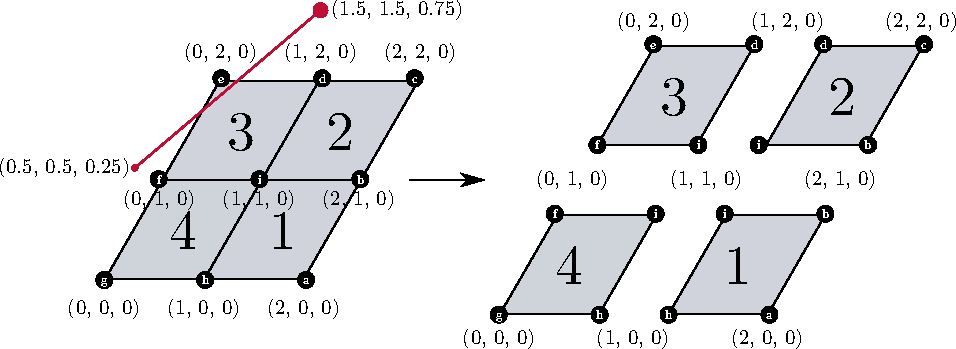
\includegraphics[width=\linewidth]{cuda_test.pdf}
		\caption[Test case for CUDA development.]{Test case for CUDA development. Dislocation line not shown in node separation as the parallelisation happens across surface elements. Not to perspective or scale.}
		\label{f:cuda_test}
	\end{figure}
	According to \cref{a:fcne} and the node labelling scheme of \cref{f:flrs} the data mapping would look like:
	\begin{align}\label{e:cuda_test}
		\vec{X}^{\textrm{SE}} = 
		\begin{split}
			\left[\overbrace{\underbrace{1,1,0,0}_{\mathbf{x_{3}}}, \underbrace{2,2,1,1}_{\mathbf{x_{4}}},
				\underbrace{1,1,0,0}_{\mathbf{x_{5}}}, \underbrace{2,2,1,1}_{\mathbf{x_{6}}}}^{x\textrm{-coord}},\right.\\
			\overbrace{\underbrace{0,1,1,0}_{\mathbf{x_{3}}}, \underbrace{0,1,1,0}_{\mathbf{x_{4}}},
				\underbrace{1,2,2,1}_{\mathbf{x_{5}}}, \underbrace{1,2,2,1}_{\mathbf{x_{6}}}}^{y\textrm{-coord}},\\
			\left.\overbrace{\underbrace{0,0,0,0}_{\mathbf{x_{3}}}, \underbrace{0,0,0,0}_{\mathbf{x_{4}}},
				\underbrace{0,0,0,0}_{\mathbf{x_{5}}}, \underbrace{0,0,0,0}_{\mathbf{x_{6}}}}^{z\textrm{-coord}}\right]
		\end{split}
	\end{align}
	In general the number of indices in the array would be $ 3 \times e \times n $ where $ e $ is the number of surface elements, $ n $ the number of nodes per element and 3 the number of spatial dimensions.
	%
	\section{Thread Block Size Optimisation}
	\href{http://docs.nvidia.com/cuda/cuda-c-best-practices-guide/index.html#memory-optimizations}{http://docs.nvidia.com/cuda/cuda-c-best-practices-guide/index.html\#memory-optimizations}
	\href{http://docs.nvidia.com/cuda/cuda-c-best-practices-guide/index.html#execution-configuration-optimizations}{http://docs.nvidia.com/cuda/cuda-c-best-practices-guide/index.html\#execution-configuration-optimizations}
	\savearabiccounter
% References
%\renewcommand{\bibname}{References} % Change bibliography name to References.
\bibliographystyle{unsrtnat}
\bibliography{bib}
\savearabiccounter
% Appendices
\appendix
% TODO #5
\chapter{Best Practices}\label{c:best_practices}
	This chapter defines the best practices that will make improve the development and testing pipeline by defining rules and standards that facilitate collaboration.
	\section{Filesystem}\label{c:best_practices:s:filesystem}
		All files must be within \texttt{/project\_name}. 
		\begin{enumerate}
			\item All files must be within \texttt{/project\_name},\\
				  \texttt{\textasciitilde/} = \texttt{project\_name/}, \\
				  \texttt{\textasciitilde/\textasciitilde/} = \texttt{project\_name/src/} or \texttt{project\_name/dev/}.
			\item Release code must be within \texttt{\textasciitilde/src/}.
			\item Development code must be within \texttt{\textasciitilde/dev/}.
			\item Test data must be within \texttt{\textasciitilde/tests/}.
			\item Documentation must be within \texttt{\textasciitilde/\textasciitilde/doc/}.
			\item Examples must be within \texttt{\textasciitilde/\textasciitilde/exmp/}.
			\item External libraries must be within \texttt{\textasciitilde/lib/}.
			\item Generated images must be within \texttt{\textasciitilde/\textasciitilde/images/}.
			\item Old versions recordkeeping must be within \texttt{\textasciitilde/prv/va.b.c/}.
		\end{enumerate}
	%
	\section{Versioning}\label{c:best_practices:s:versioning}
		\begin{enumerate}
			\item Use a version control system like \href{https://github.com/}{GitHub} or \href{https://pastebin.com/}{PasteBin}.
			\item There must be a master branch that is only changed when the code is stable and bug free.
			\item Development branches should be exploited as seen fit without making things overly convoluted.
			\item Commits must be as bug free and regular as possible. When to commit is left to the developer's discresion.
			\item Commit messages should be as descriptive as possible.
			\item Versions should be specified as \texttt{va.b.c} where \texttt{a}, \texttt{b}, \texttt{c} = integers. The three levels are \texttt{a} = release version (usable, bug free code), \texttt{b} = beta version (code that is undergoing testing), \texttt{c} = alpha version (code that is under active development).
		\end{enumerate}
	%	 
	\section{Documentation}\label{c:best_practices:s:documentation}
		\subsection{Commenting}\label{c:best_practices:s:documentation:ss:commenting}
			Every codefile must be appropriately commented by meeting the following guidelines.
			\begin{enumerate}
				\item The start of each codefile must have a heading detailing the creator, date of creation and edit history (date and name of editor).
				\item Below the heading there must be a general explanation of the code. It must state any procedures, structures, objects and how they are to be utilised. Any backward or forward dependencies must be stated.
				\item Below the description and edit history any relevant literature must be mentioned (dois are preferred). Must be as detailed as possible, include equation numbers/ranges if necessary.
				\item The start of every procedure has an explanation of its purpose, inputs, outputs and inputs-outputs.
				\item Particularly complicated code blocks must have an in-depth explanation of what it does. Comment each line if necessary.
				\item Corrections or additions must be explicitly bounded by comments at the start and end of the change. Both bounding comments must have the author's name and the date. Below the starting comment, there should be an explanation of the change. Any punctual comments can be made as normal.
			\end{enumerate}
		\subsection{README}\label{c:best_practices:s:documentation:ss:readme}
			Every codefile must have an associated \textsc{readme} \texttt{.tex} document that documents the codefile's contents. It must meet the following guidelines as appropriate.
			\begin{enumerate}
				\item The name must be that of the file it documents (minus the extension of course).
				\item Description and overall explanation of the codefile's purpose.
				\item Overall flow chart or pseudo code describing the file's purpose.
				\item Document the codefile's procedures. This means describing and explaining their corresponding inputs, outputs, inputs-outputs, forwards and backwards dependencies, and flow charts or pseudo codes.
				\item Unit test designs and results for each procedure. If appropriate also include those of integral tests.
			\end{enumerate}
			The codefile may also be appended at the end of documentation if desired (the \texttt{minted} package is highly recommended).
	%
	\section{Modularisation}\label{c:best_practices:s:modularisation}
		\begin{enumerate}
			\item Code repetition must be kept to a \emph{strict} minimum. Any piece of code that will be reused must be modularised.
			\item Procedures must be as self-sufficient as possible \emph{without} repeating code. If repeating code is necessary, replace it with a procedure that is to be repeatedly called instead. Minimising repeated code $\ggg$ procedure self-sufficiency.
		\end{enumerate}
	%
	\section{Coding Style}\label{c:best_practices:s:naming_conventions}
		All names must meet the following guidelines.
		\begin{enumerate}
			\item Indent appropriately. Four space tabs are a good compromise between code necking and readability.
			\item Minimise the use of nested code blocks, use intrisics, libraries or create procedures instead.
			\item Break up lines that are uncomfortably long, typically anything over 80--100 characters.
			\item Names should be appropriately descriptive and human readable.
			\item All code and names must be systematic and logical.
			\item the use of upper cases should be reserved for parameters (\texttt{const} variables in C).
			\item Delimit words with ``\texttt{\_}'' \emph{not} case changes.
			\item Long and descriptive $\ggg$ short and cryptic.
		\end{enumerate}
		\subsection{Filenames}\label{c:best_practices:s:naming_conventions:ss:filenames}
			\begin{enumerate}
				\item If old versions are to be kept, the old \emph{stable} versions of file must have the date of last modification appended \emph{suffixed} after the file extension in the \texttt{\_yyyymmdd} format. For example, if the stable version of the release code \texttt{hello\_world\_parallel.c} was last modified on April 25, 2017 it should be archived as\\ \texttt{hello\_world\_parallel.c\_20170425}.
			\end{enumerate}
		\subsection{Variables, Structures and Objects}\label{c:best_practices:s:naming_conventions:ss:variables_structures_objects}
			\begin{enumerate}
				\item Only counters and indices can be single letter variables.
				\item Structure and object \emph{definitions} are \emph{suffixed} with \texttt{\_s} and \texttt{\_o} respectively.
				\item Inputs, outputs and input-outputs to procedures must be \emph{prefixed} with \texttt{i\_}, \texttt{o\_} and \texttt{io\_} respectively.
			\end{enumerate}
		\subsection{Procedures}\label{c:best_practices:s:naming_conventions:ss:procedures}
			\begin{enumerate}
				\item Functions and subroutines must be \emph{prefixed} with \texttt{f\_} and \texttt{s\_} respectively.
			\end{enumerate}
\chapter{Coupling Discrete Dislocation Dynamics to Finite Element Methods}

% \inputminted[breaklines, linenos, fontsize=\normalsize]{matlab}{../EasyDD/extract_node_plane.m}

% \inputminted[breaklines, linenos, fontsize=\normalsize]{matlab}{../EasyDD/extract_node_planes.m}

% \inputminted[breaklines, linenos, fontsize=\normalsize]{matlab}{../EasyDD/analytic_traction.m}

\chapter{Implementation of Analytical Forces Induced by Dislocations on Linear Rectangular Surface Elements}
\section{Serial C Code MEX File}
%\inputminted[breaklines, linenos, fontsize=\normalsize]{c}{../../../Dropbox/Daniel/DDLabFEM/nodalForce/nodal_surface_force_linear_rectangle_arr_unix.c}
\section{Parallel CUDA C Code MEX File}
\savearabiccounter

\chapter{Implementation of Analytical Forces Induced by Dislocations on Quadratic Triangular Surface Elements}
	\section{Serial C Code MEX File}
	%\inputminted[breaklines, linenos, fontsize=\normalsize]{c}{../../../Dropbox/Daniel/DDLabFEM/nodalForce/nodal_surface_force_quad_triangle_qp.c}
	\section{Parallel CUDA C Code MEX File}

\chapter{Talks}
	\section{Durham July 12--14 2017}
		Bridging the gap between the microscopic and macroscopic world is an on-going challenge for science and technology. If we hope to understand complex emergent phenomena we need to study systems that blur the line between micro and macro. In materials science, one such area is the study of extended defects called dislocations; whose nucleation and movement mediate the permanent deformation of materials. These large, high energy defects present very complex and long ranged interactions with each other, crystal boundaries, impurities, free surfaces, and themselves. As such, their dynamics are difficult to study experimentally. So we make justified assumptions and simplifications and create models that let us study them in detail. However if our models are to prove useful in real applications, they must be continually refined and improved by weakening assumptions and removing simplifications. Unfortunately, with increased refinement comes increased computational cost and new challenges. Therefore, finding faster alternatives that do not sacrifice accuracy is of the utmost importance---better yet if the alternatives are more accurate or exact. With the advent of increasingly accessible graphics processor units (GPUs) typically used in video gaming, the power of parallel processing is no longer exclusive to researchers with access to supercomputers. In this talk we will discuss the GPU implementation of exact solutions for the forces dislocations exert on the surfaces of materials.
% Backmatter
% TODO #3:
\begin{romanpages}
	\printglossary[nonumberlist]
	\phantomsection
	\addcontentsline{toc}{chapter}{Index} % Add index to the table of contents (toc).
	\printindex
\end{romanpages}
\end{document}